\chapter{Adaptive Strategies}

In this section, we focus on adaptive LES of flow over a surging airfoil at different conditions. Problem setup, and baseline results including vortex detection and tracking, are first presented using the non-adapated mesh. We also present active flow control cases in the form of active reflex camber. Next, we present the three adaptive strategies and corresponding results. 

\chapter{LES of Flow Over Surging Airfoil}
\label{chapter:baseline_results}

In this chapter, we focus on LES of flow over a surging airfoil at different conditions. Problem setup as well as results including vortex detection and tracking are presented. A non-adapated mesh is used here to get familiar with the features of the current problem at different conditions, while results on the adapted meshes are presented in the next chapter.
% We also present active flow control cases in the form of active reflex camber. 

%\section{LES of Flow Over Surging Airfoil}
%\section{Adaptive LES of Flow Over Surging Airfoil}
%\section{LES of Flow Over Surging Airfoils including Active Reflex}


\section{Problem Setup}
\label{sec:problem_setup_baseline}

%TODO: Add U_rel velocity profile with t_tilde

A schematic of the problem setup is shown in Figure~\ref{fig:SetUpSketch}, where $U_\infty$ is the free-stream or mean velocity and $\alpha$ is the angle of attack.

\begin{figure}[H]
\centering
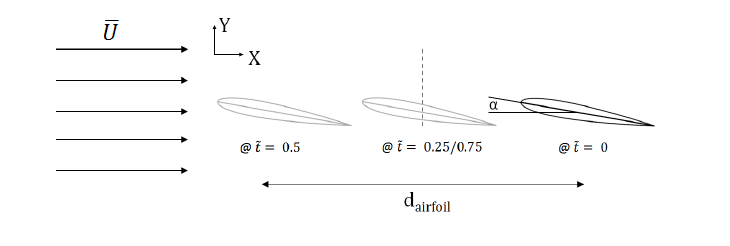
\includegraphics[width=0.8\textwidth]{figures/Setup/Setup.png}
\caption{Schematic of the surging airfoil problem}
\label{fig:SetUpSketch}
\end{figure}

The airfoil motion is set as follows
\begin{equation}
\label{eq:displacement}
  d_{airfoil} = A cos(2\pi f t) =  Acos(2\pi t/T) = Acos(2\pi\tilde{t})
\end{equation}

\noindent where $A$ is the amplitude and $T=1/f$ is the time period of the oscillation.
The variable $\tilde{t}$ is the fractional part in the oscillation cycle and is defined as $\tilde{t}=\{t/T\} = t/T - \lfloor t/T \rfloor$ (where $\lfloor \cdot \rfloor$ is the floor function).

The (non-dimensional) relative velocity is expressed as
\begin{equation}
\label{eq:relVelocity}
  \tilde{U}_{rel} = U_{rel}/U_\infty = 1 - U_{airfoil}/U_\infty = (1+\mu_{sect} sin(2\pi\tilde{t}))
\end{equation}
\noindent where $\mu_{sect}$ is the sectional advance ratio.
Note that for a sectional advance ratio above $1.0$ a negative relative velocity or a reversed flow condition is attained (e.g., at this radial section/location of the blade).
Under the reversed flow condition the relative flow is from the (geometric) trailing edge to the leading edge of the airfoil.

At $\tilde{t}$=0, with $\psi$=$0^\circ$ or $\psi$=$0^\circ$ (where, $\psi$ is the phase in the oscillation cycle and $\psi$ is the azimuthal position of the blade), the relative velocity is the free-stream velocity (i.e., $U_\infty$).
The same holds at $\tilde{t}$=0.5 or $\psi$=$180^\circ$.
At $\tilde{t}$=0.25 or $\psi$=$90^\circ$, the airfoil is at the maximum relative velocity and at $\tilde{t}$=0.75 or $\psi$=$270^\circ$ is at the minimum relative velocity.
Advancing part of the cycle is defined between $\tilde{t}$=0 or $\psi$=$0^\circ$ and $\tilde{t}$=0.5 or $\psi$=$180^\circ$, while retreating part is between $\tilde{t}$=0.5 or $\psi$=$180^\circ$ and $\tilde{t}$=1.0 or $\psi$=$360^\circ$ (or back to $\psi$=$0^\circ$).

The free-stream or mean Reynolds number is defined as: $Re=U_\infty C/\nu$, where $C$ is the chord.
The reduced frequency is defined as $k=\pi f C/U_\infty$ while the amplitude is related as $A = \frac{\mu_{sect} C}{2k}$.

\section{Summary of Cases}
\label{sec:baseline_case_summary}

In the current study, the reduced frequency is held fixed at $k$=0.133 while three Reynolds numbers of $Re$=40,000, 200,000 and 1,000,000 are considered together with two sectional advance ratios of $\mu_{sect}$=1.0 and 1.2, i.e., six cases are considered in total.
The angle of attack of the airfoil is set to 6$^\circ$.
Note that we considered the Reynolds number of $Re$=40,000 in a previous study~\cite{bib:kocher_scitech2017} that was selected in accordance with the experiments conducted in \cite{bib:granlund2016} where the airfoil was placed in a constant flow and oscillated in the streamwise direction.
The six cases are summarized in Table~\ref{table:summary_cases}.

\begin{table}[H]
\centering
\caption{Summary of cases}
\label{table:summary_cases}
\begin{tabular}{|l|c|c|c|c|}
\hline
Airfoil   & $\alpha$ & $k$ & $\mu_{sect}$ & $Re$ \\
\hline
\hline
NACA 0012 & 6$^\circ$ & $0.133$ & \{1.0, 1.2\} & \{40,000,\; 200,000,\; 1,000,000\} \\
\hline
\end{tabular}
\end{table}

The computational domain is set to be $100C$ x $50C$ x $0.2C$.
At the inlet, a constant free-stream velocity is applied
(note that the airfoil is moved sinusoidally in the streamwise direction).
No-slip condition is prescribed on the moving airfoil.
The top and bottom surfaces are set as slip walls.
Side surfaces in the spanwise direction (i.e., front and back surfaces) are imposed to be periodic.
A natural pressure condition is used at the outlet.
A second-order implicit time integration scheme, e.g., see \cite{bib:tran2017b}, is employed with about 1,440 steps in an oscillation cycle.

%TODO: give justification for this mesh ... typical LES resolution for a BL (based on highest Reynolds number in the surge cycle) ... but indicate no consideration taken for other flow features such as separation and LEV.
An unstructured hybrid/boundary layer mesh is used.
The mesh is comprised of hex and wedge elements which is generated by first generating a mesh on the front surface and by subsequently applying an extrusion in the spanwise direction. This (non-adapted) mesh is used for all cases listed above. Again, this is done to get familiar with the features of the current problem at different conditions, while mesh adaptivity is investigated in the next chapter. The non-adapted mesh is constructed by following recommended practices in terms of mesh resolution on the surface of the airfoil and around it, as discussed below.

Refinement zones are placed around the airfoil to resolve the flow structures of interest, see Figure \ref{fig:mesh} (where three refinement zones are noted).
In the finest refinement zone (Z1), mesh size is set to be $C/256$.
In the subsequent two zones (Z2 and Z3), it is set to be $C/128$ and $C/64$, respectively.
In the spanwise direction, 50 extruded elements are used.
A layered and graded mesh (with geometric growth) is used around the airfoil surface, see Figure \ref{fig:mesh2}.
The first layer height is set to be $\mathcal{O}(10^{-5} C)$ such that it is below 1 in wall units for all cases.
Similarly, mesh spacing on the airfoil surface in the streamwise and spanwise directions is set to be below 80 and 50 in wall units, respectively, for the XXX (which Reynolds number and which part of the cycle).
Overall the mesh contains about 6.2 million nodes and 10.8 million elements.

\begin{figure}[H]
\centering
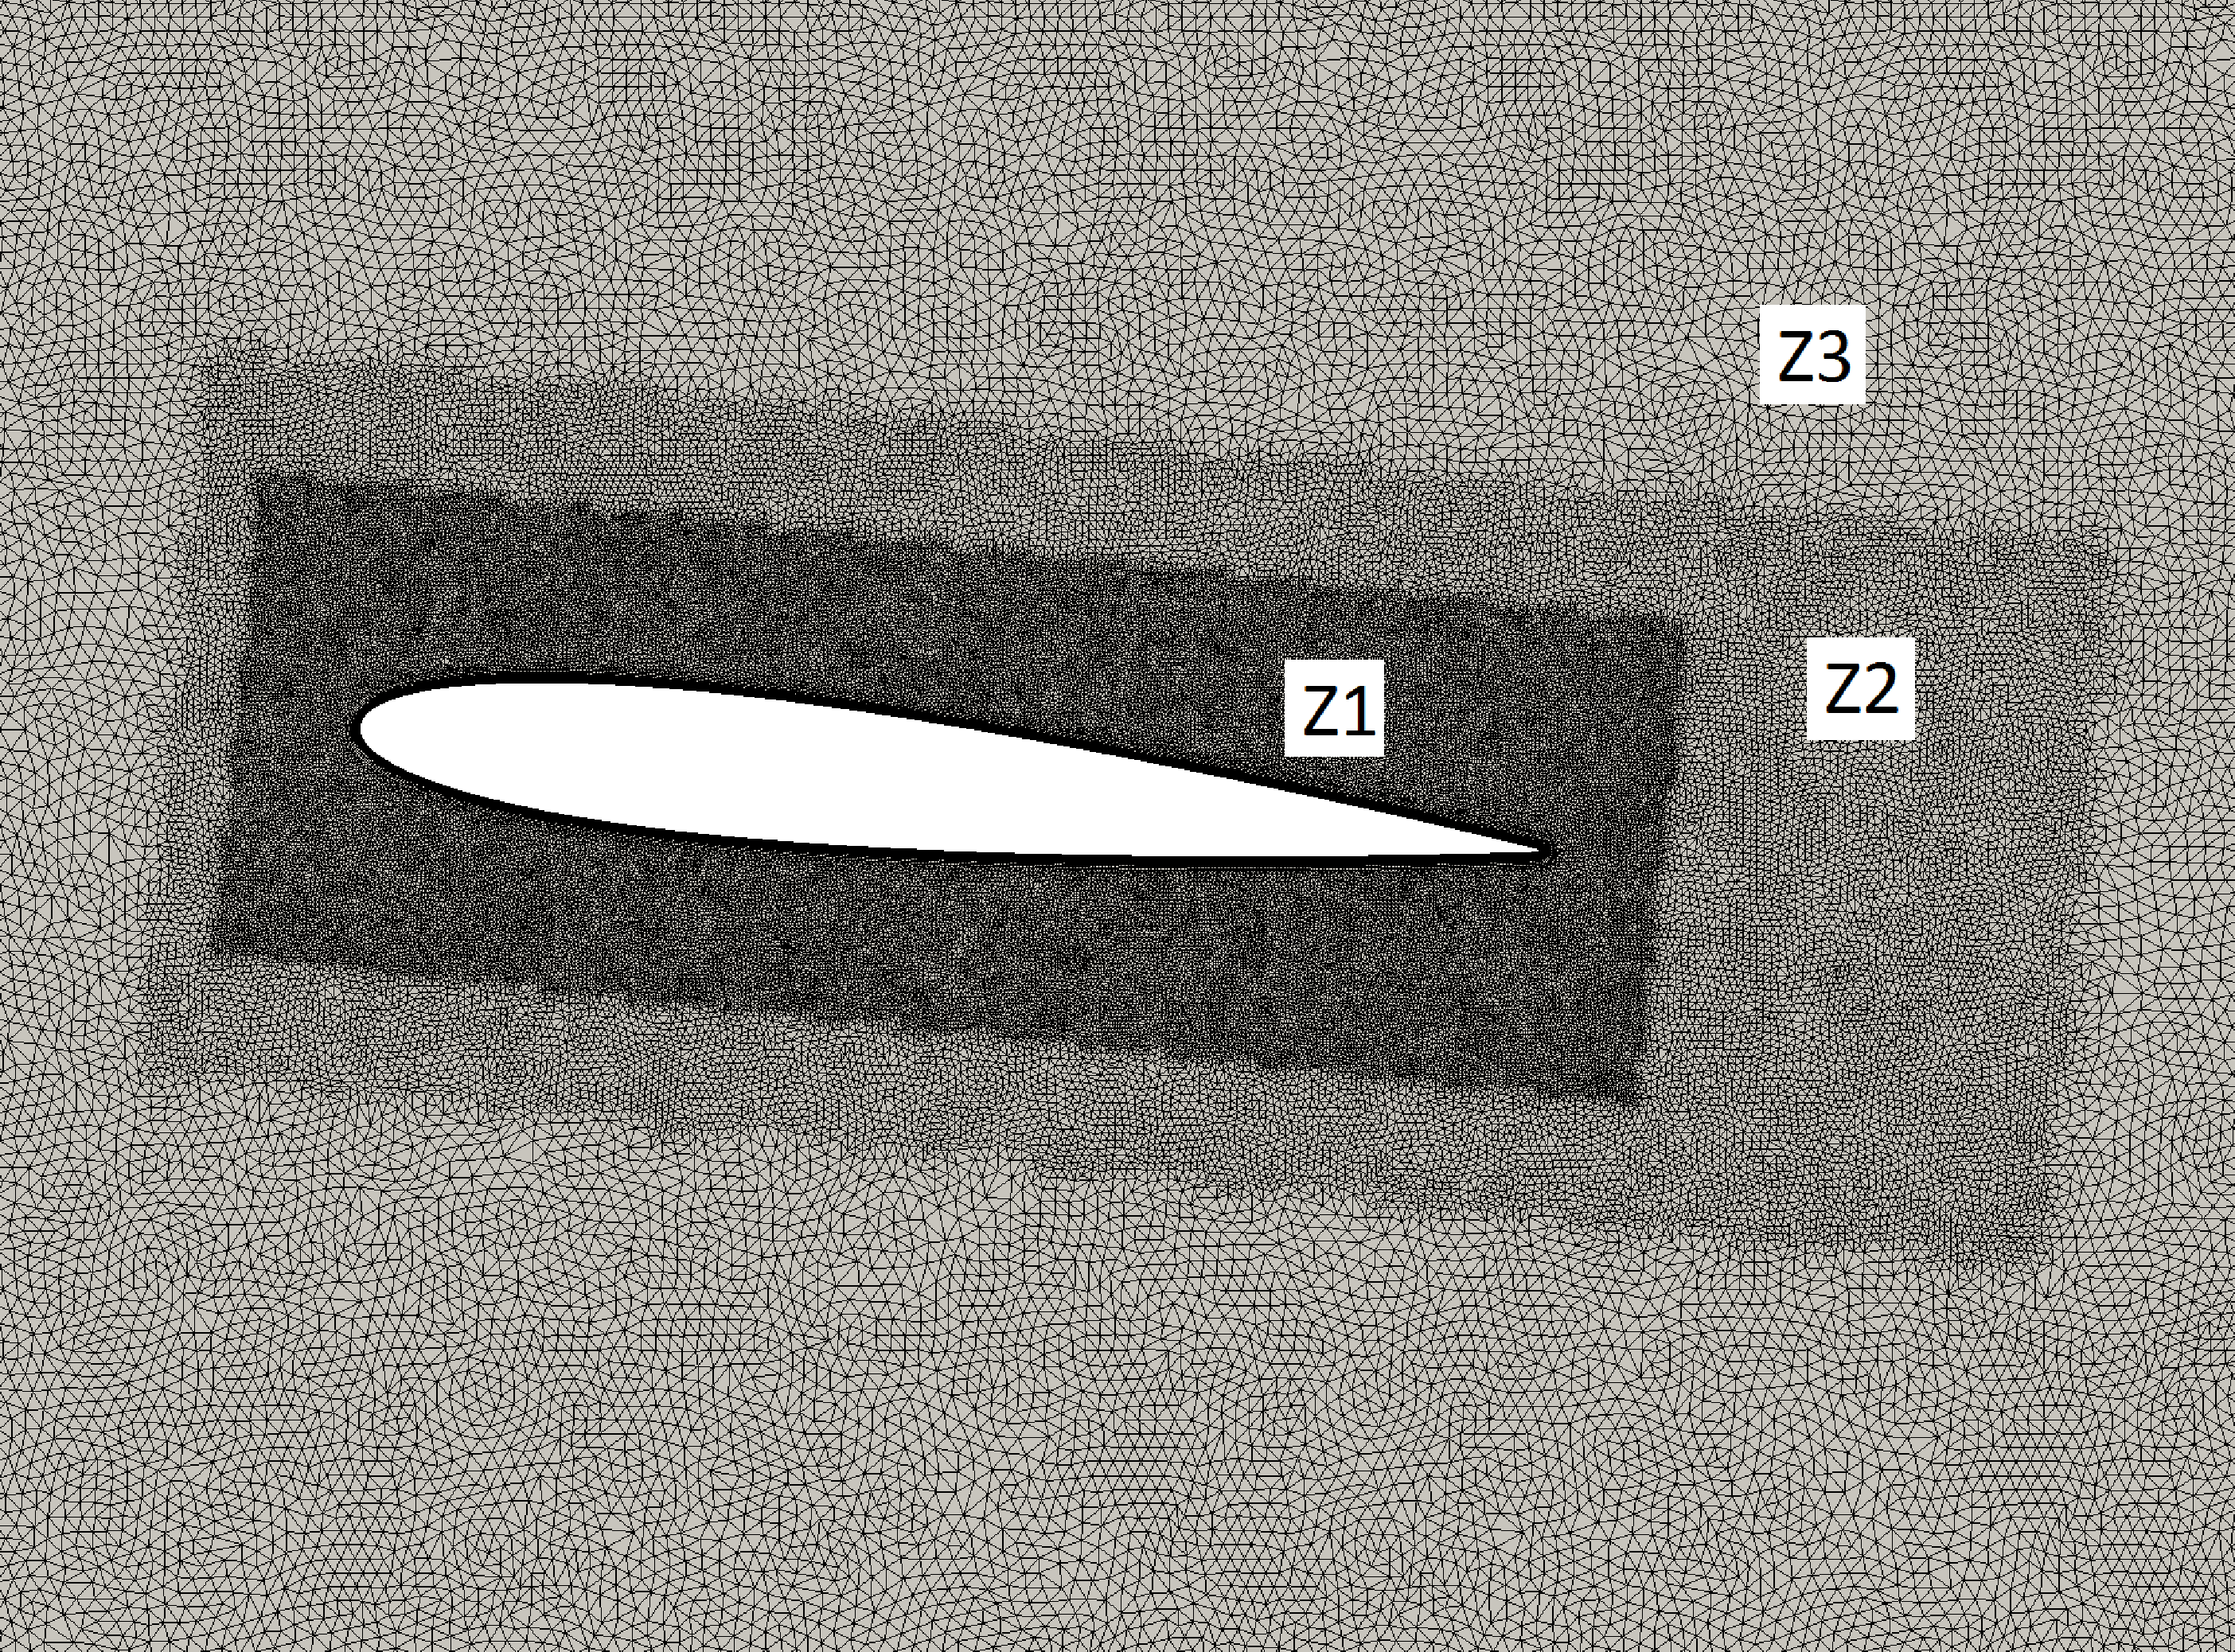
\includegraphics[width=0.7\textwidth]{figures/Setup/mesh_screenshot.pdf}
\caption{Mesh around the airfoil with refinement zones}
\label{fig:mesh}
\end{figure}

\begin{figure}[H]
\centering
\includegraphics[width=0.45\textwidth]{figures/Setup/mesh_LE.pdf}
\includegraphics[width=0.45\textwidth]{figures/Setup/mesh_TE.pdf}
\caption{Layered and graded mesh around the leading edge and trailing edge of the airfoil}
\label{fig:mesh2}
\end{figure}

\section{Results and Discussion}

\subsection{Force Response}

\begin{figure}[H]
	\begin{subfigure}{0.5\textwidth}
		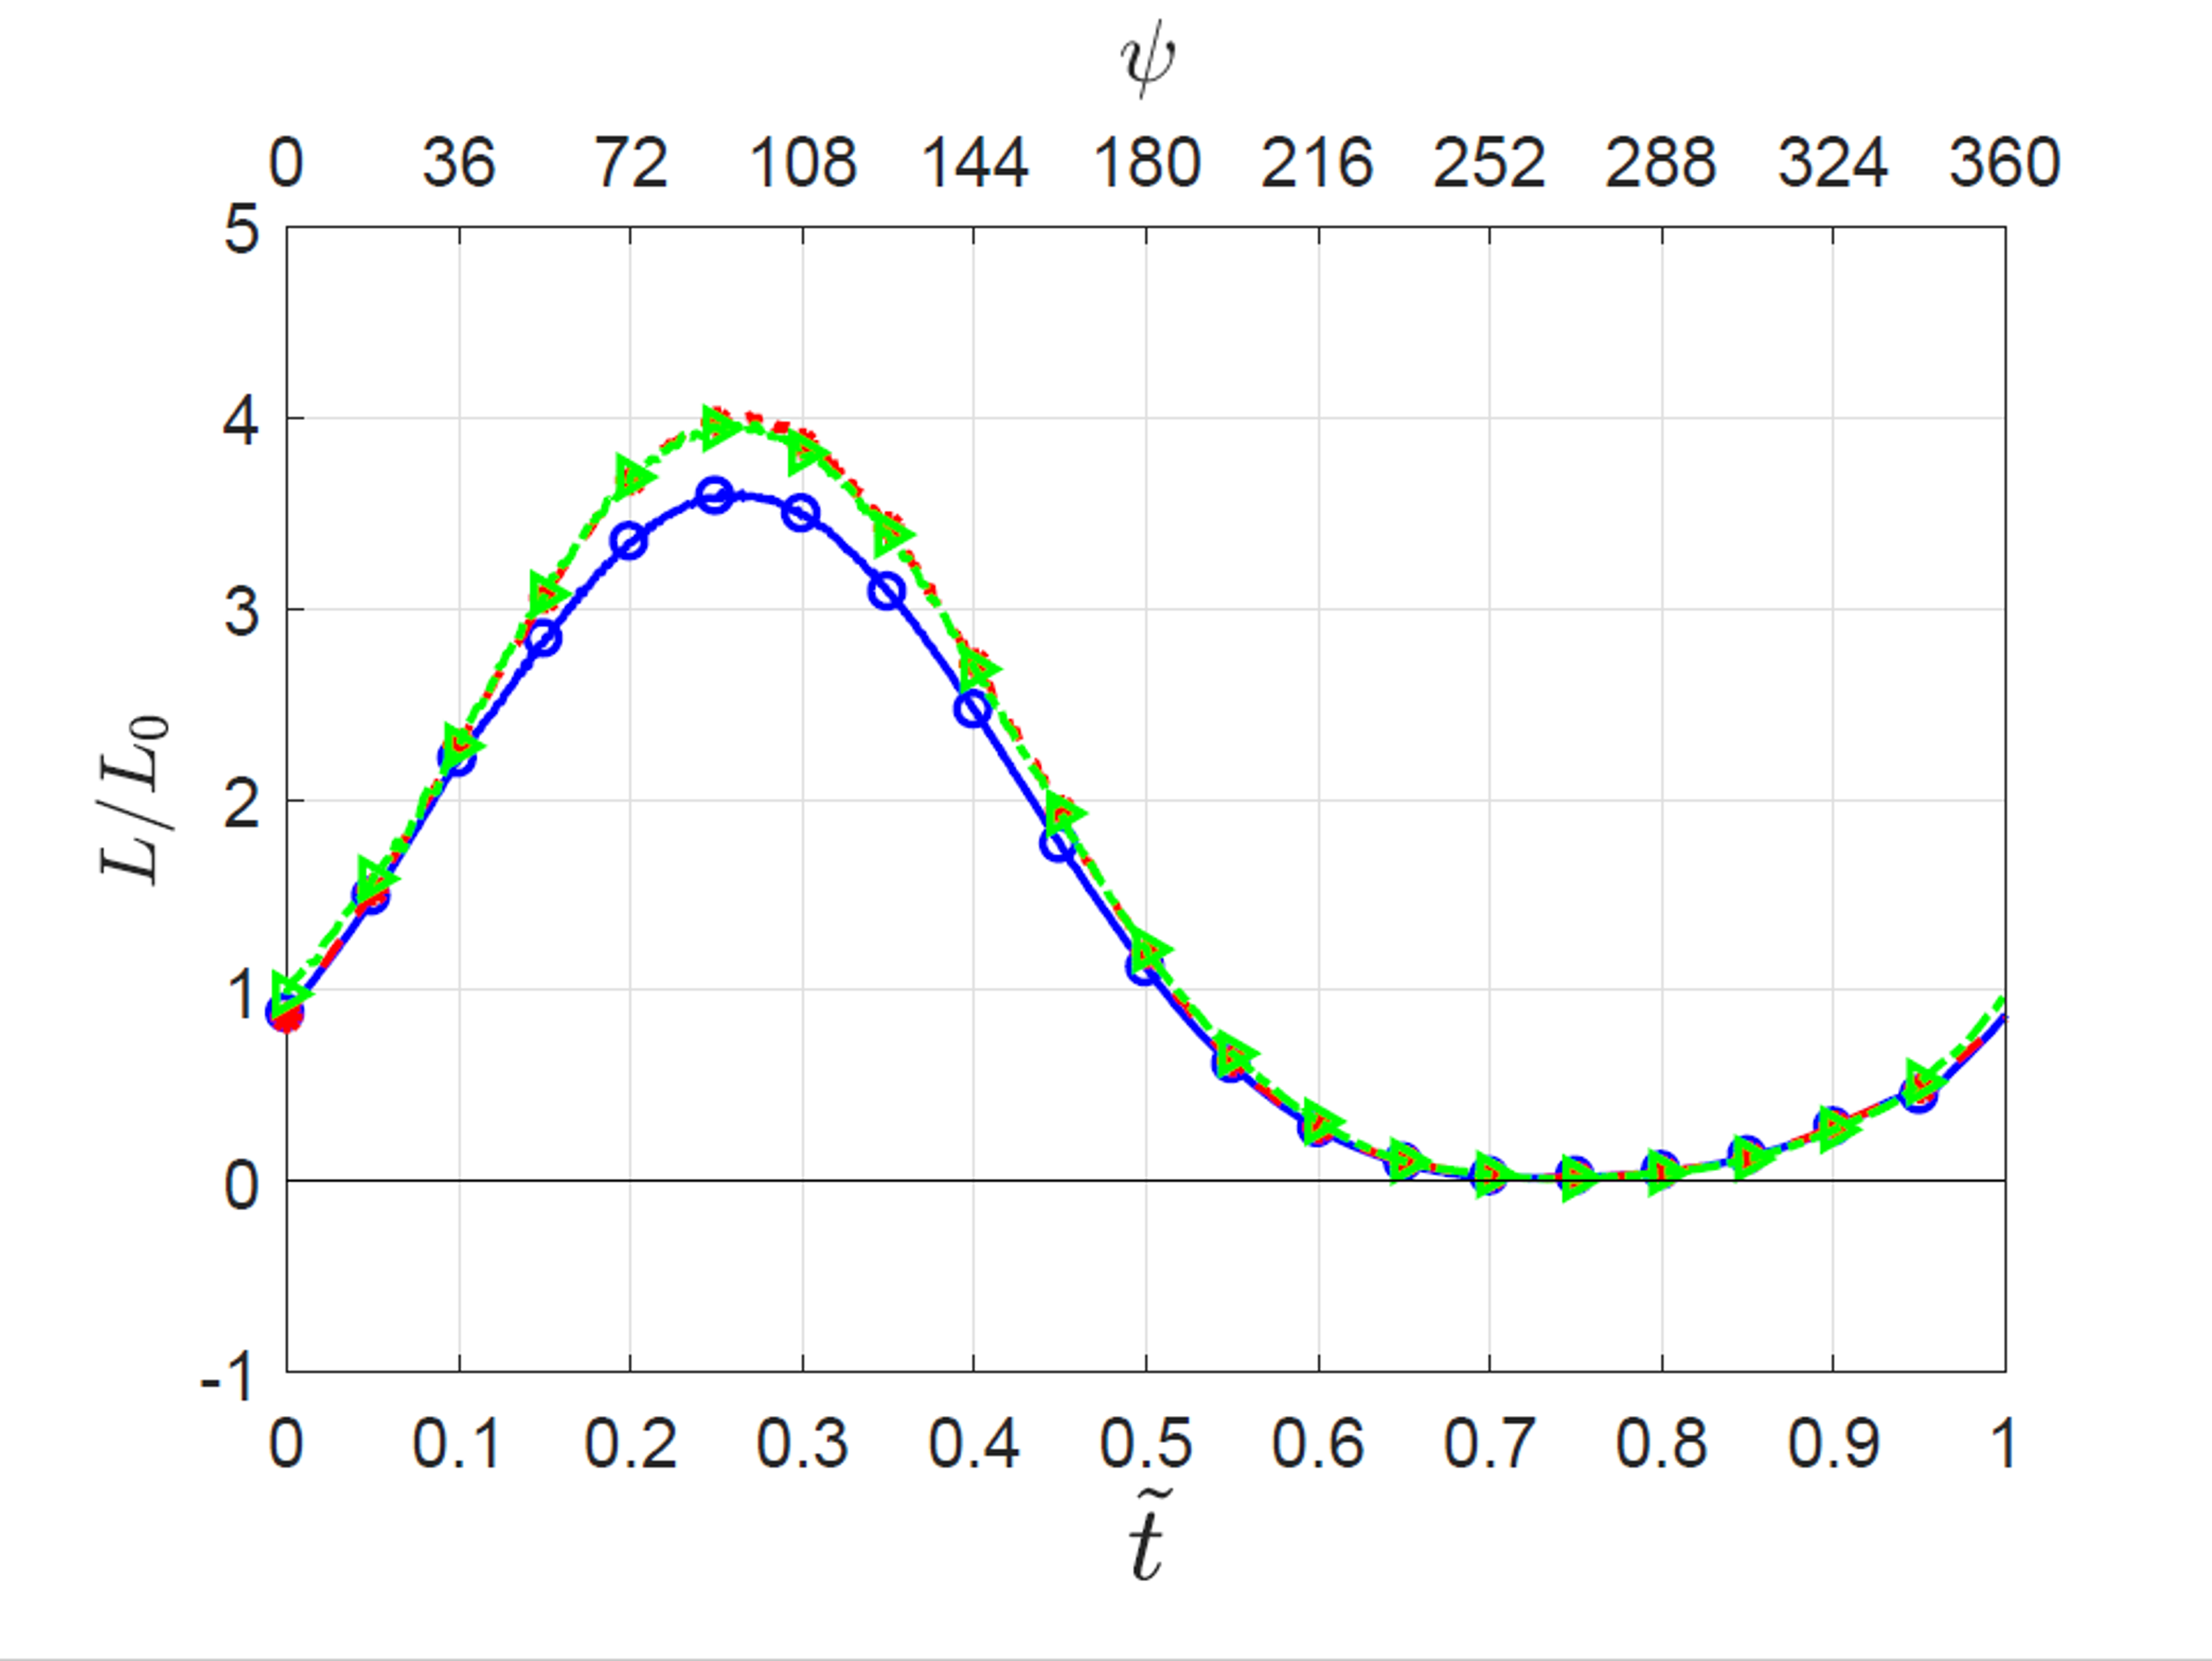
\includegraphics[width=1\textwidth]{figures/lift_Re_effect_lambda_1pt0.png}
		\subcaption{$\mu_{sect} = 1.0$}
		\label{fig:lift_Re_comparision_lambda_1p0}
	\end{subfigure}
 	\begin{subfigure}{0.5\textwidth}
		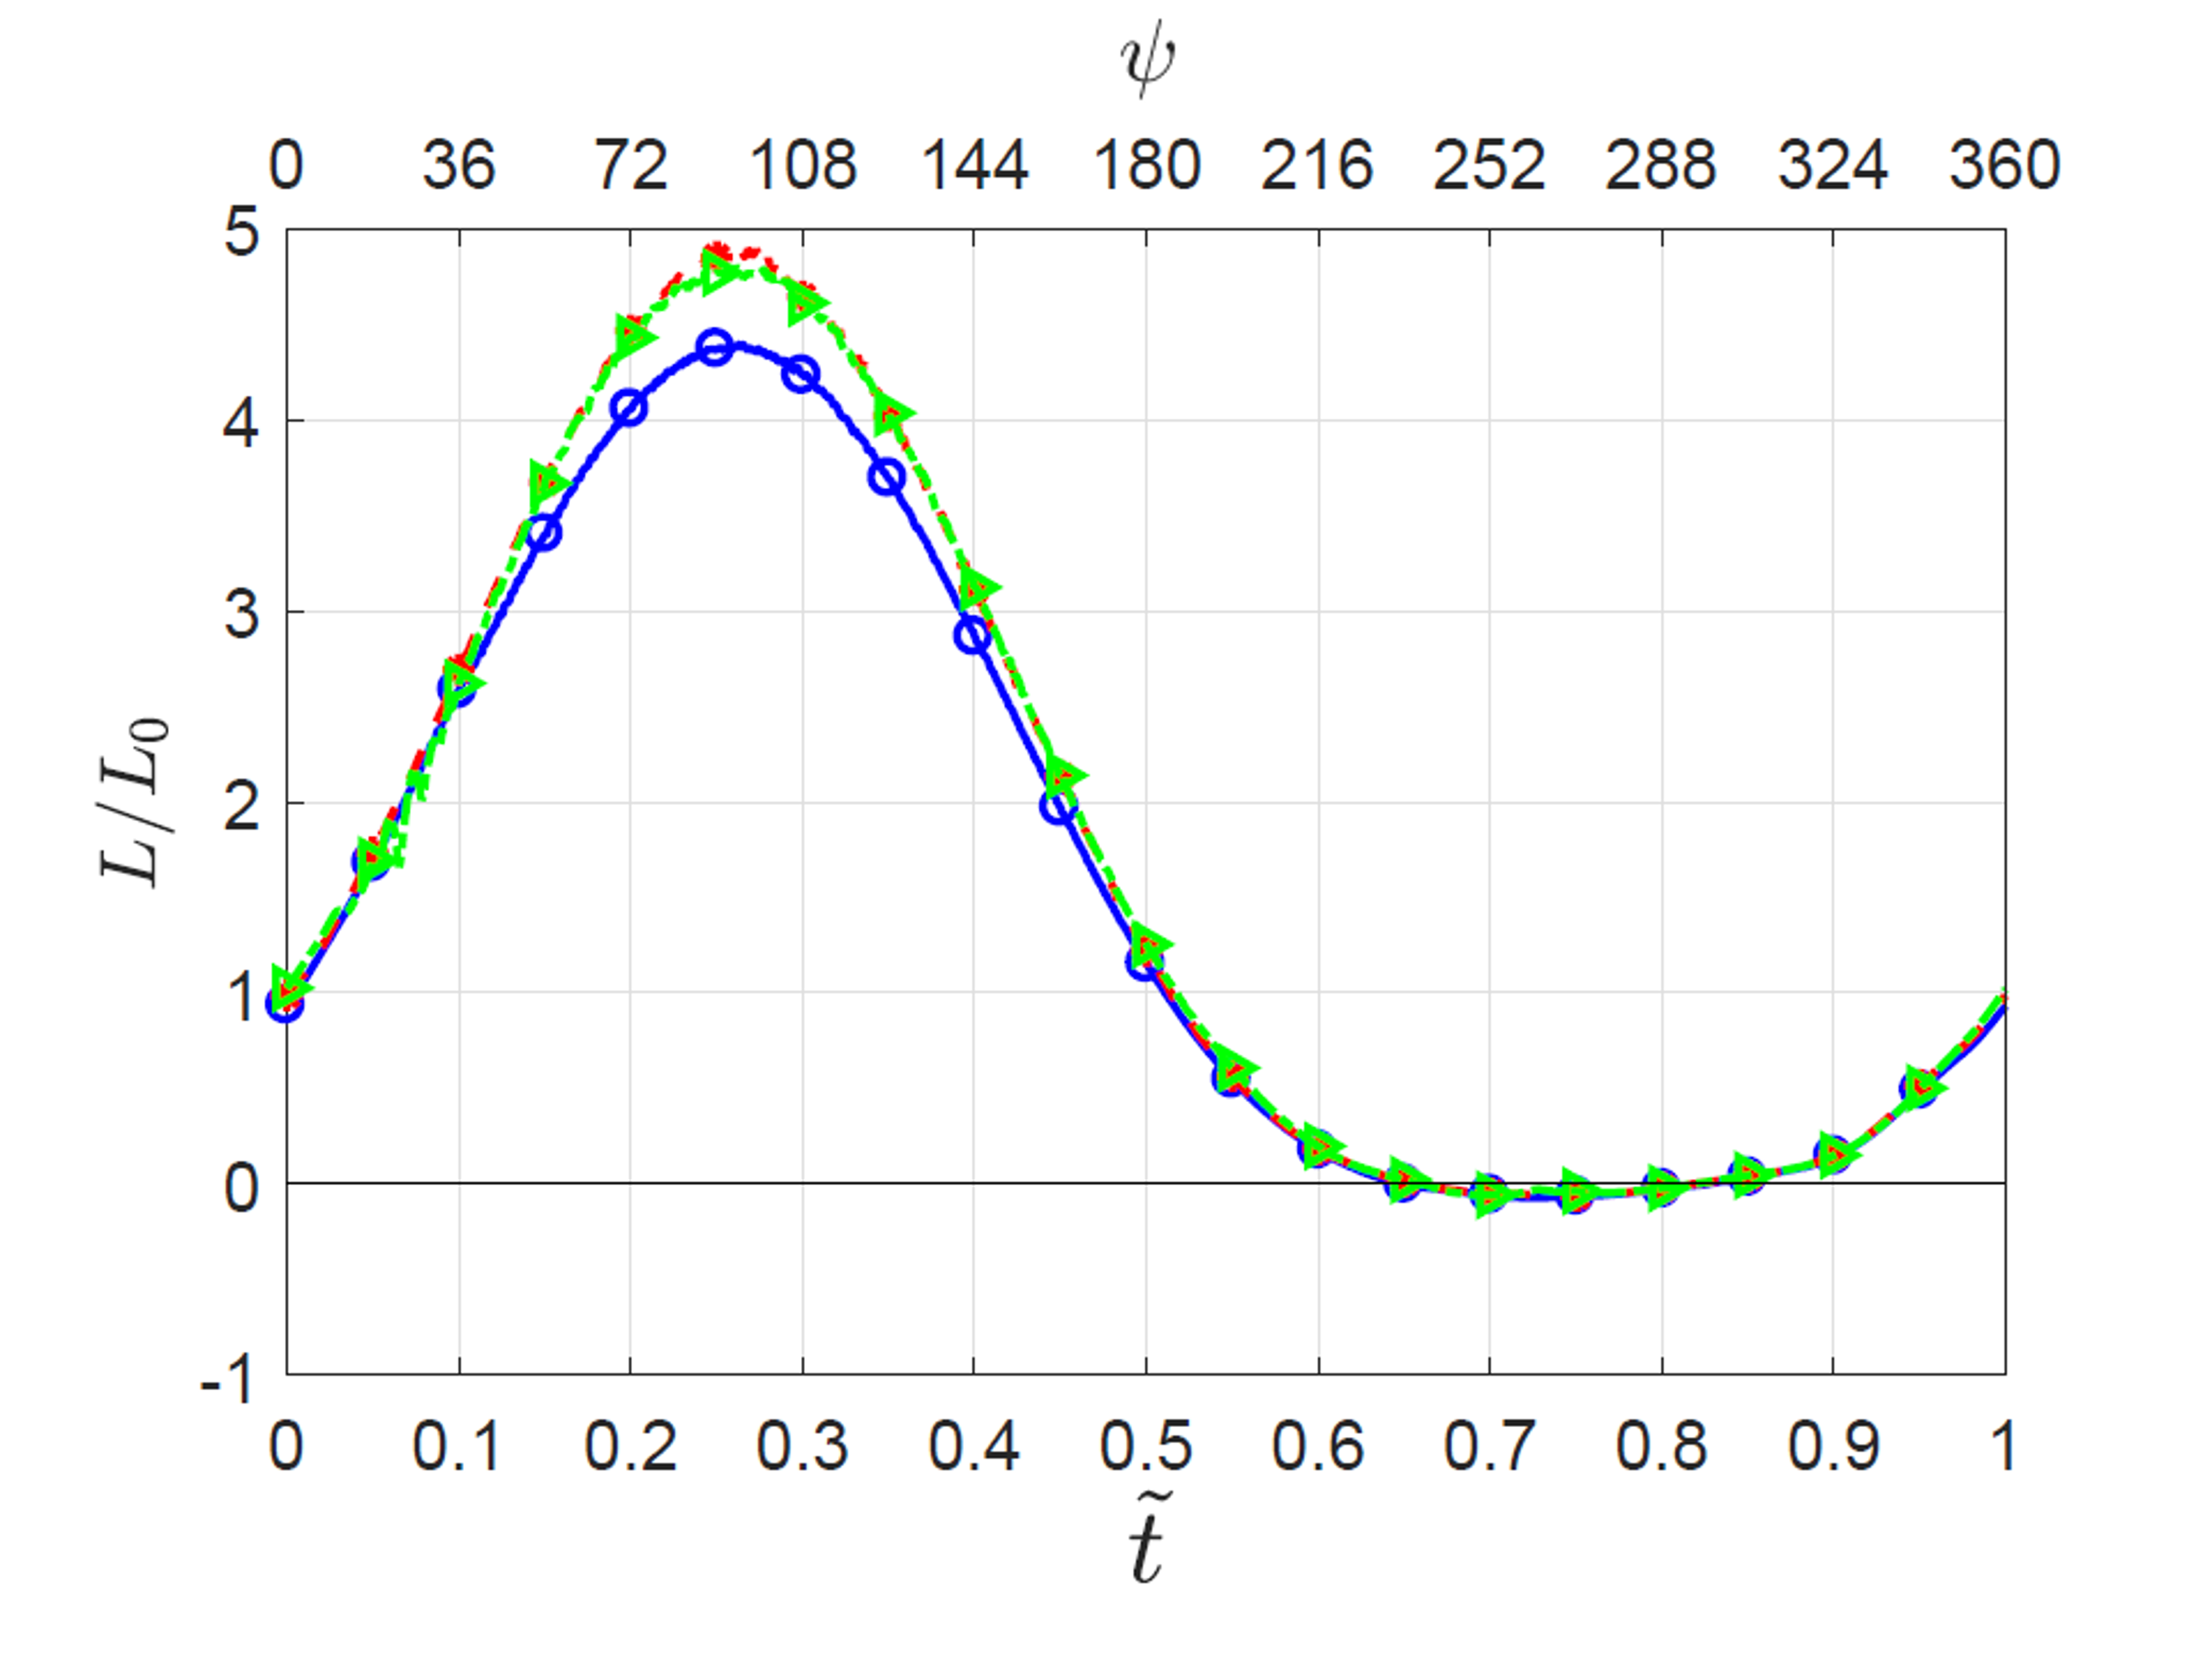
\includegraphics[width=1\textwidth]{figures/lift_Re_effect_lambda_1pt2.png}
        \subcaption{$\mu_{sect} = 1.2$}
		\label{fig:lift_Re_comparision_lambda_1p2}
	\end{subfigure}

 	\caption{Normalized lift force for $Re$=40,000 (green line with open triangles), 200,000 (red line with solid circles) and 1,000,000 (blue line with open circles) at $\mu_{sect}$=1.0 and 1.2}
 	\label{fig:lift_comparison}
\end{figure}

Lift force is shown in Figure \ref{fig:lift_comparison}.
Lift is normalized by its static counterpart, i.e., $L_0$ is the average or steady lift for the static airfoil at the mean Reynolds number over the surging cycle.
This normalization was used in our previous study with $Re$=40,000~\cite{bib:kocher_scitech2017} to compare against the experimental data of \cite{bib:granlund2016}, where a good agreement was shown between the experimental and simulation data.
Data is phase averaged over 4 cycles.
%%%We note that the averaged drag data exhibits fluctuations which is due to the presence of a turbulent flow, especially during the advancing phase of the cycle with a higher relative velocity or Reynolds number.
%%%However, these fluctuations are marginal in nature and averaging over additional cycles will be useful.

Overall, the lift force follows a similar qualitative trend for all the cases.
Maximum lift is achieved at $\tilde{t}=0.25$, which is expected as the airfoil achieves maximum relative velocity at that point.
After $\tilde{t}=0.25$, the lift starts decreasing as the airfoil begins to decelerate and enters the retreating phase. 
The lift keeps decreasing till about $\tilde{t}=0.65$ and plateaus or reaches a value close to zero during the middle of the retreating phase (i.e., around $\tilde{t}=0.75$ when the airfoil is at its minimum relative velocity).
We note that for both advance ratios of $\mu_{sect}$=1.0 and 1.2 a zero relative velocity is attained and for the higher advance ratio of $\mu_{sect}$=1.2 the relative velocity also becomes negative.
Lift starts to recover after $\tilde{t}=0.75$ as the airfoil starts accelerating again.
For each advance ratio, the normalized lift during the advancing phase for $Re$=1,000,000 is slightly smaller compared to the other two Reynolds numbers, see Figure \ref{fig:lift_Re_comparision_lambda_1p0} or Figure \ref{fig:lift_Re_comparision_lambda_1p2}.
The normalized lift is very similar between $Re$=40,000 and 200,000 cases.
The peak normalized lift is about 9\% lower for the highest Reynolds number case as compared to the lower Reynolds number cases for each advance ratio.
On the other hand, for a given Reynolds number the normalized lift is higher for the higher advance ratio, which is expected due to the higher dynamic pressure in any given instance or phase in the surging cycle.
The peak normalized lift is about 21\% higher for the higher advance ratio case as compared to the lower advance ratio case for each Reynolds number, which is the difference in the peak dynamic pressure between the two advance ratios.

\subsection{Flowfield: Spanwise Vorticity}

In this section, we present spanwise vorticity over the cycle at 8 different phases of $\psi$ = $195^\circ$, $225^\circ$, $240^\circ$, $255^\circ$, $270^\circ$, $315^\circ$, $330^\circ$,and $345^\circ$, which are all in the retreating part of the surging cycle.
We focus our attention on the leading edge vortex (LEV) which is the dominant flow feature.
It forms and advects during the retreating part, while in the advancing part the flow remains attached.
As noted earlier, data is phase averaged over 4 cycles.
In addition, averaging is also applied in the spanwise direction.

Figure \ref{fig:vortScreen_1pt0} shows the spanwise vorticity for the lower advance ratio of $\mu_{sect}$=1.0.
The voriticy range is selected to be [-10,10]$\times U_\infty /C$.
At $\psi$=$195^\circ$, the flow over the airfoil is mostly attached, however, the boundary layer is relatively thick as the airfoil is decelerating, see Figures~\ref{fig:Re_40k_1pt0_phi195}, \ref{fig:Re_200k_1pt0_phi195} and \ref{fig:Re_1m_1pt0_phi195}.
As expected, the boundary layer is much thicker for the lowest Reynolds number of $Re$=40,000 as compared to the other two higher Reynolds numbers.

\begin{figure}[H]
	\centering
	
	\begin{subfigure}[b]{0.32\textwidth}
		\centering
		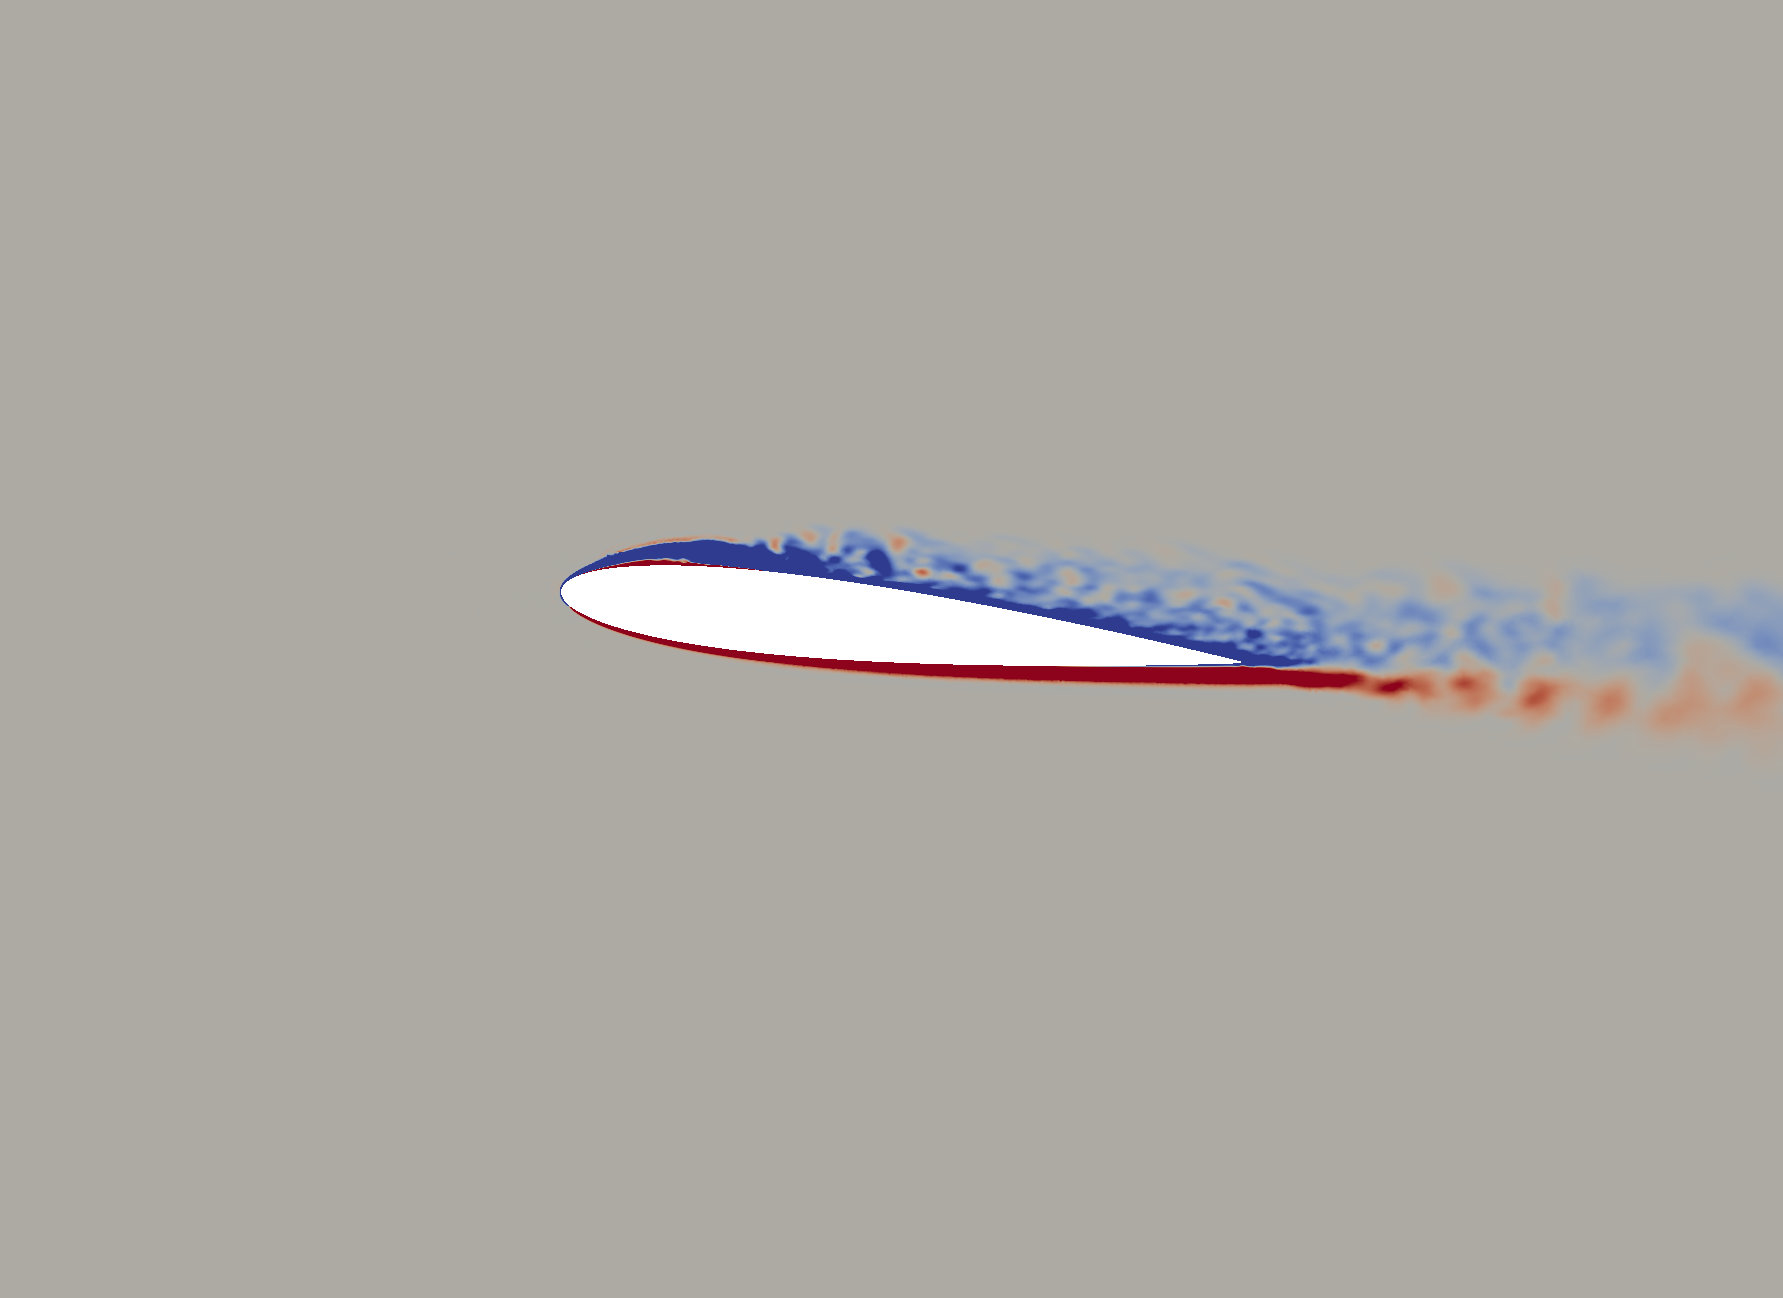
\includegraphics[width=1\textwidth]{figures/Vorticity_plots/Re_40k_1pt0/phase_195.png}
		\caption{$Re=4e4$, $\psi$ = $195^\circ$, $\tilde{t}=0.542$}
		\label{fig:Re_40k_1pt0_phi195}
	\end{subfigure}
	\begin{subfigure}[b]{0.32\textwidth}
		\centering
		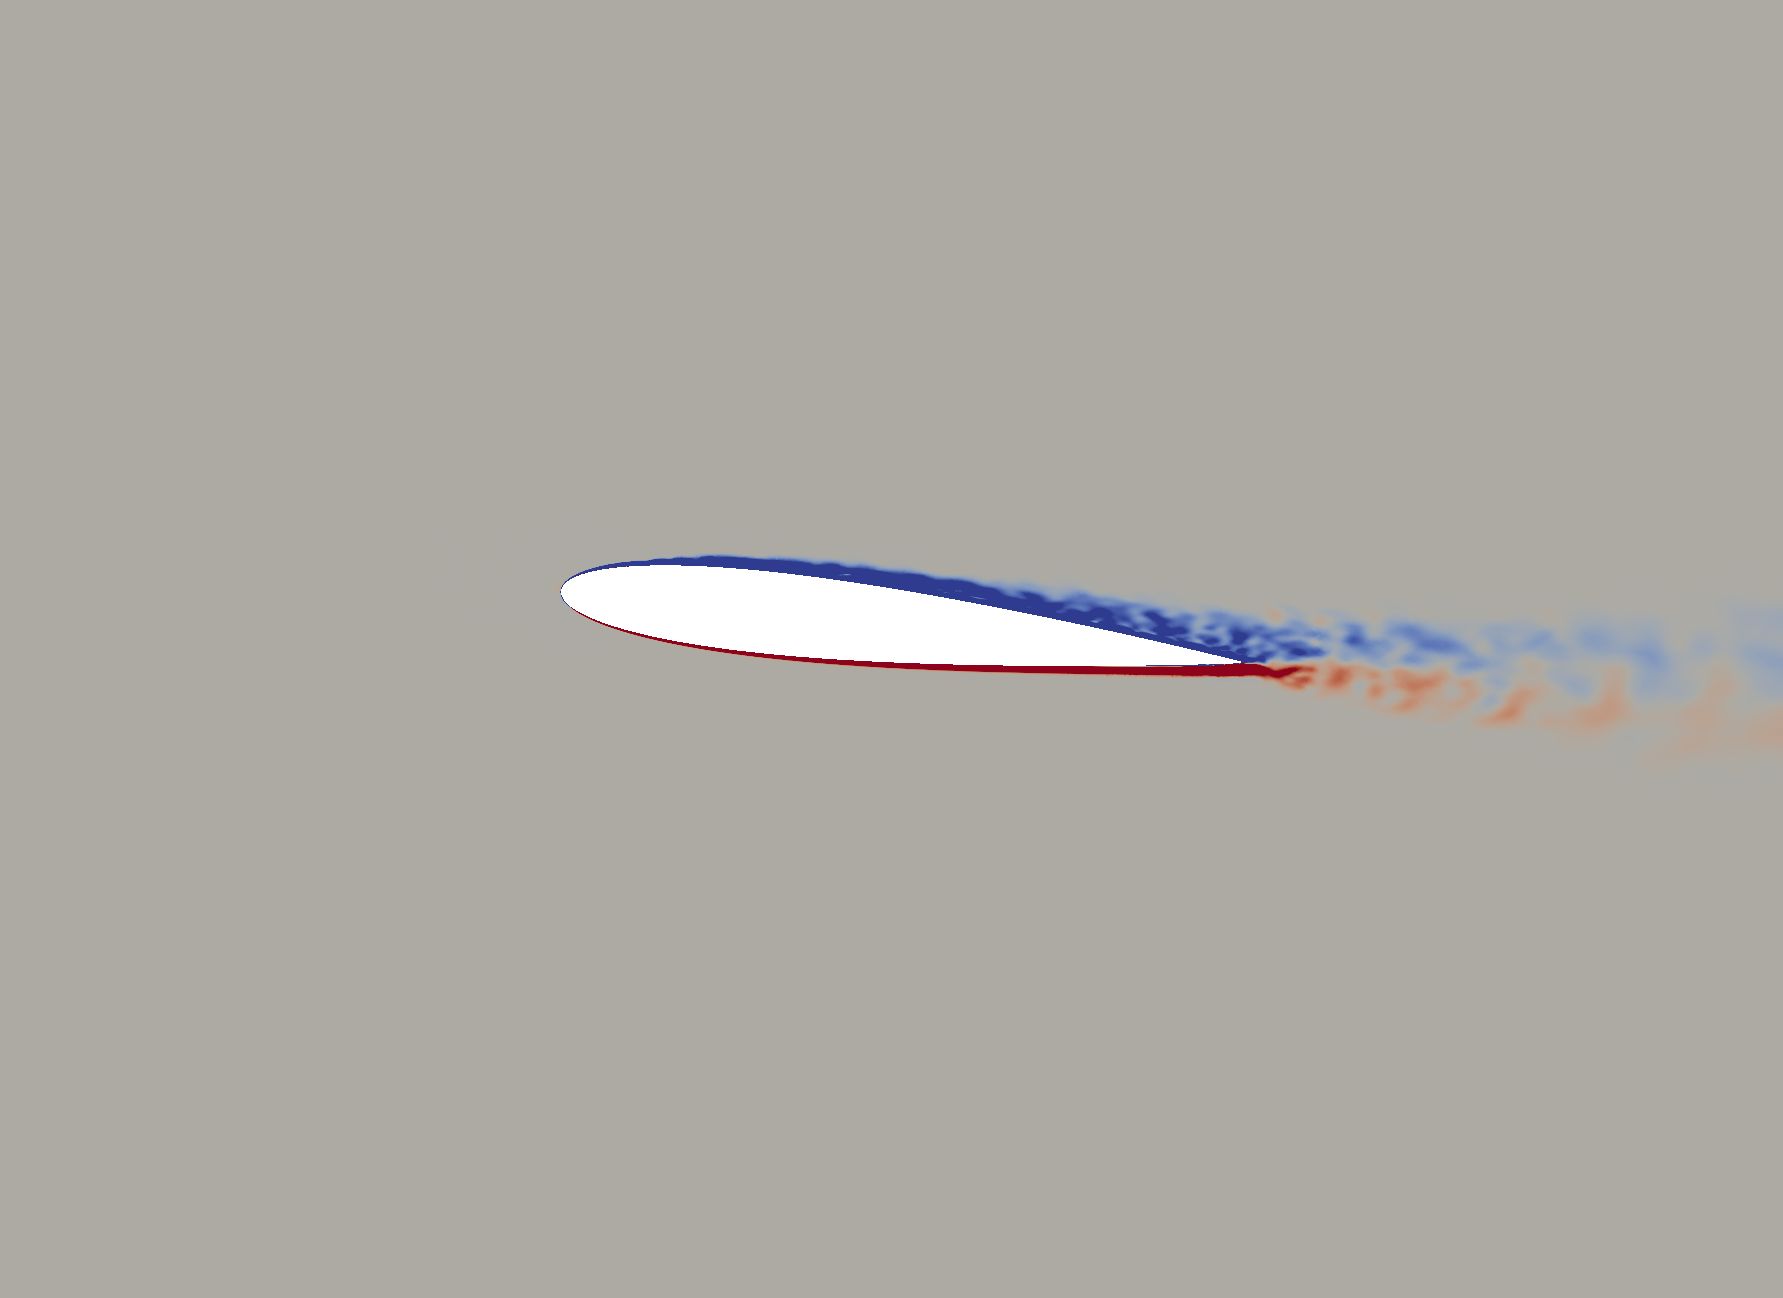
\includegraphics[width=1\textwidth]{figures/Vorticity_plots/Re_200k_1pt0/phase_195.png}
		\caption{$Re=2e5$, $\psi$ = $195^\circ$, $\tilde{t}=0.542$}
		\label{fig:Re_200k_1pt0_phi195}
	\end{subfigure}
	\begin{subfigure}[b]{0.32\textwidth}
		\centering
		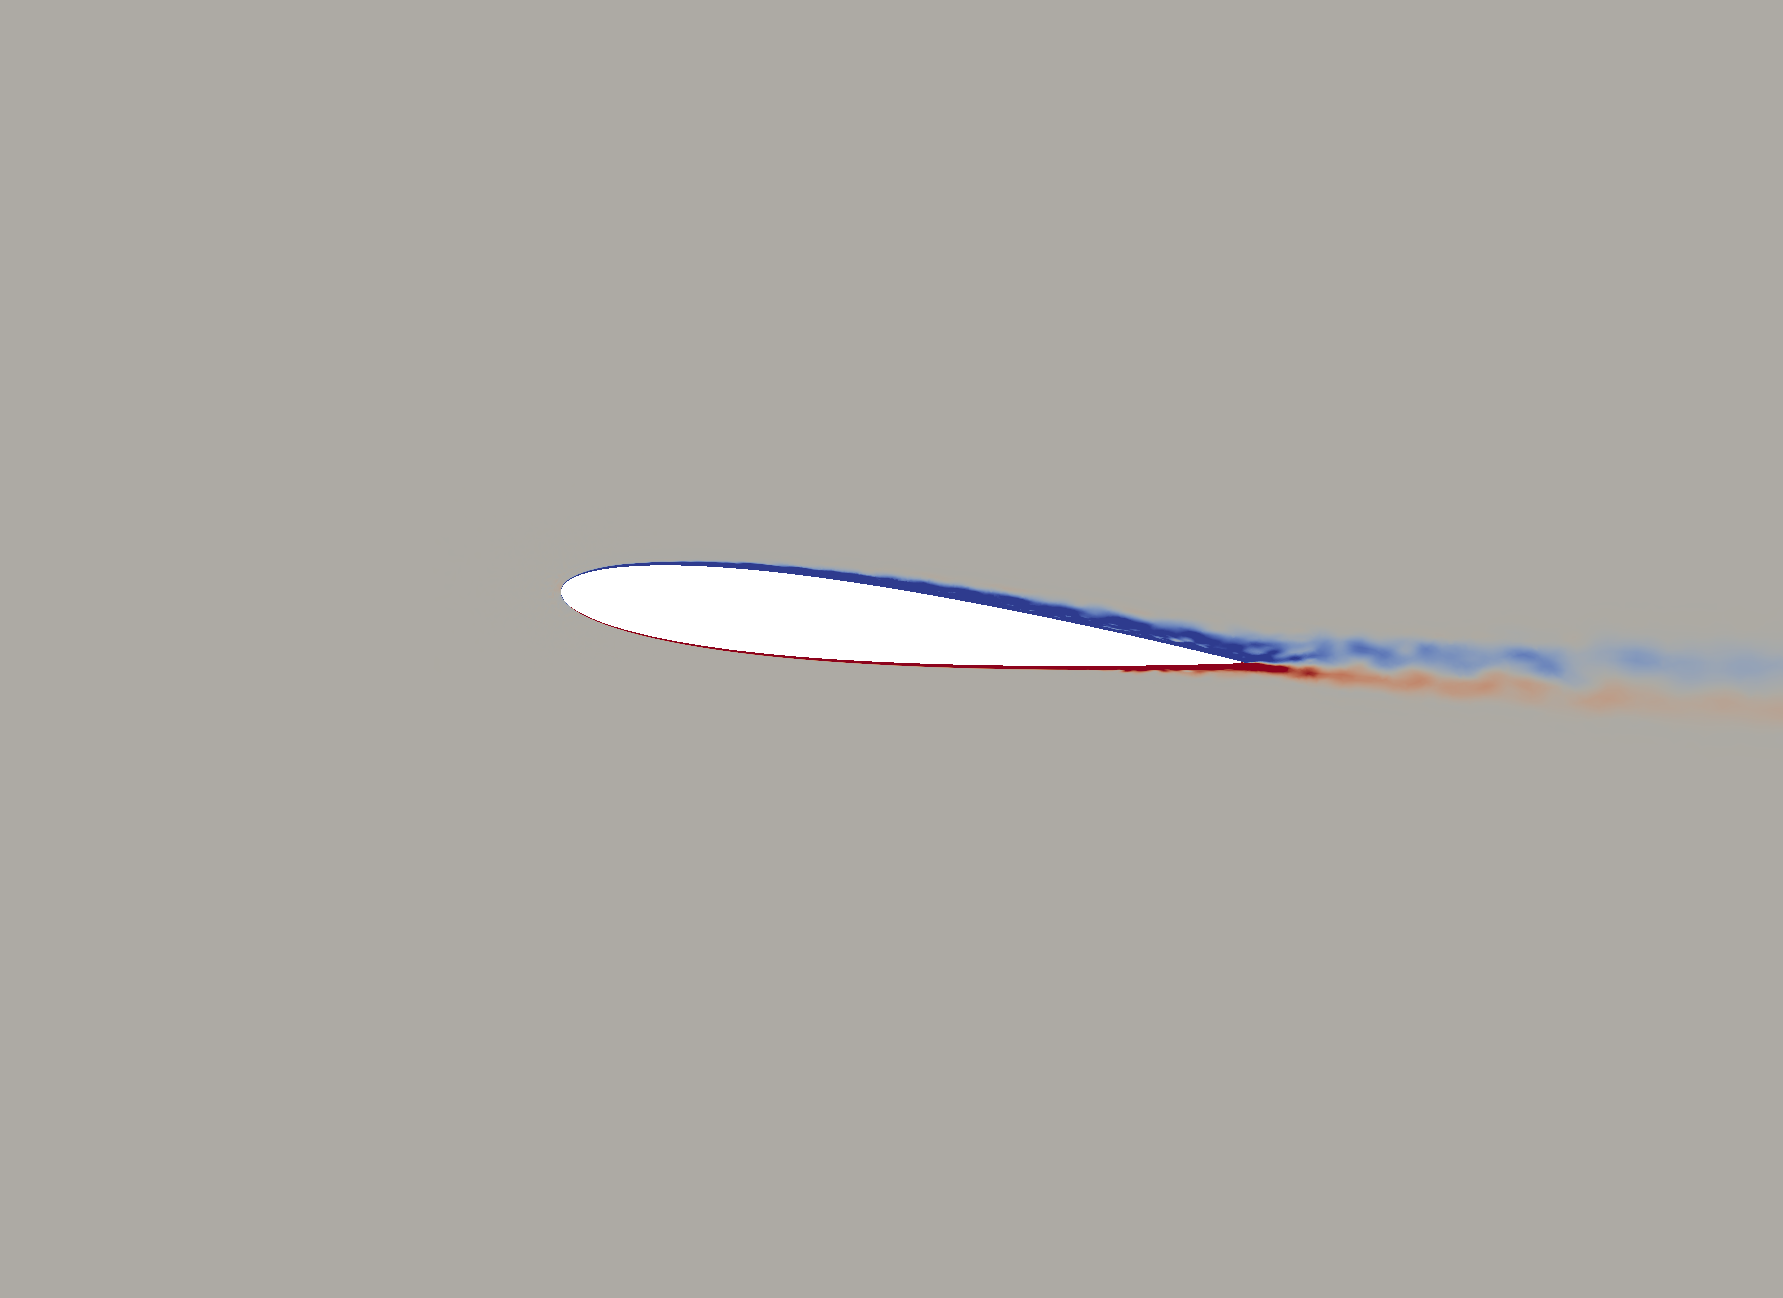
\includegraphics[width=1\textwidth]{figures/Vorticity_plots/Re_1m_1pt0/phase_195.png}
		\caption{$Re= 1e6$, $\psi$ = $195^\circ$, $\tilde{t}=0.542$}
		\label{fig:Re_1m_1pt0_phi195}
	\end{subfigure}
	
	\begin{subfigure}[b]{0.32\textwidth}
		\centering
		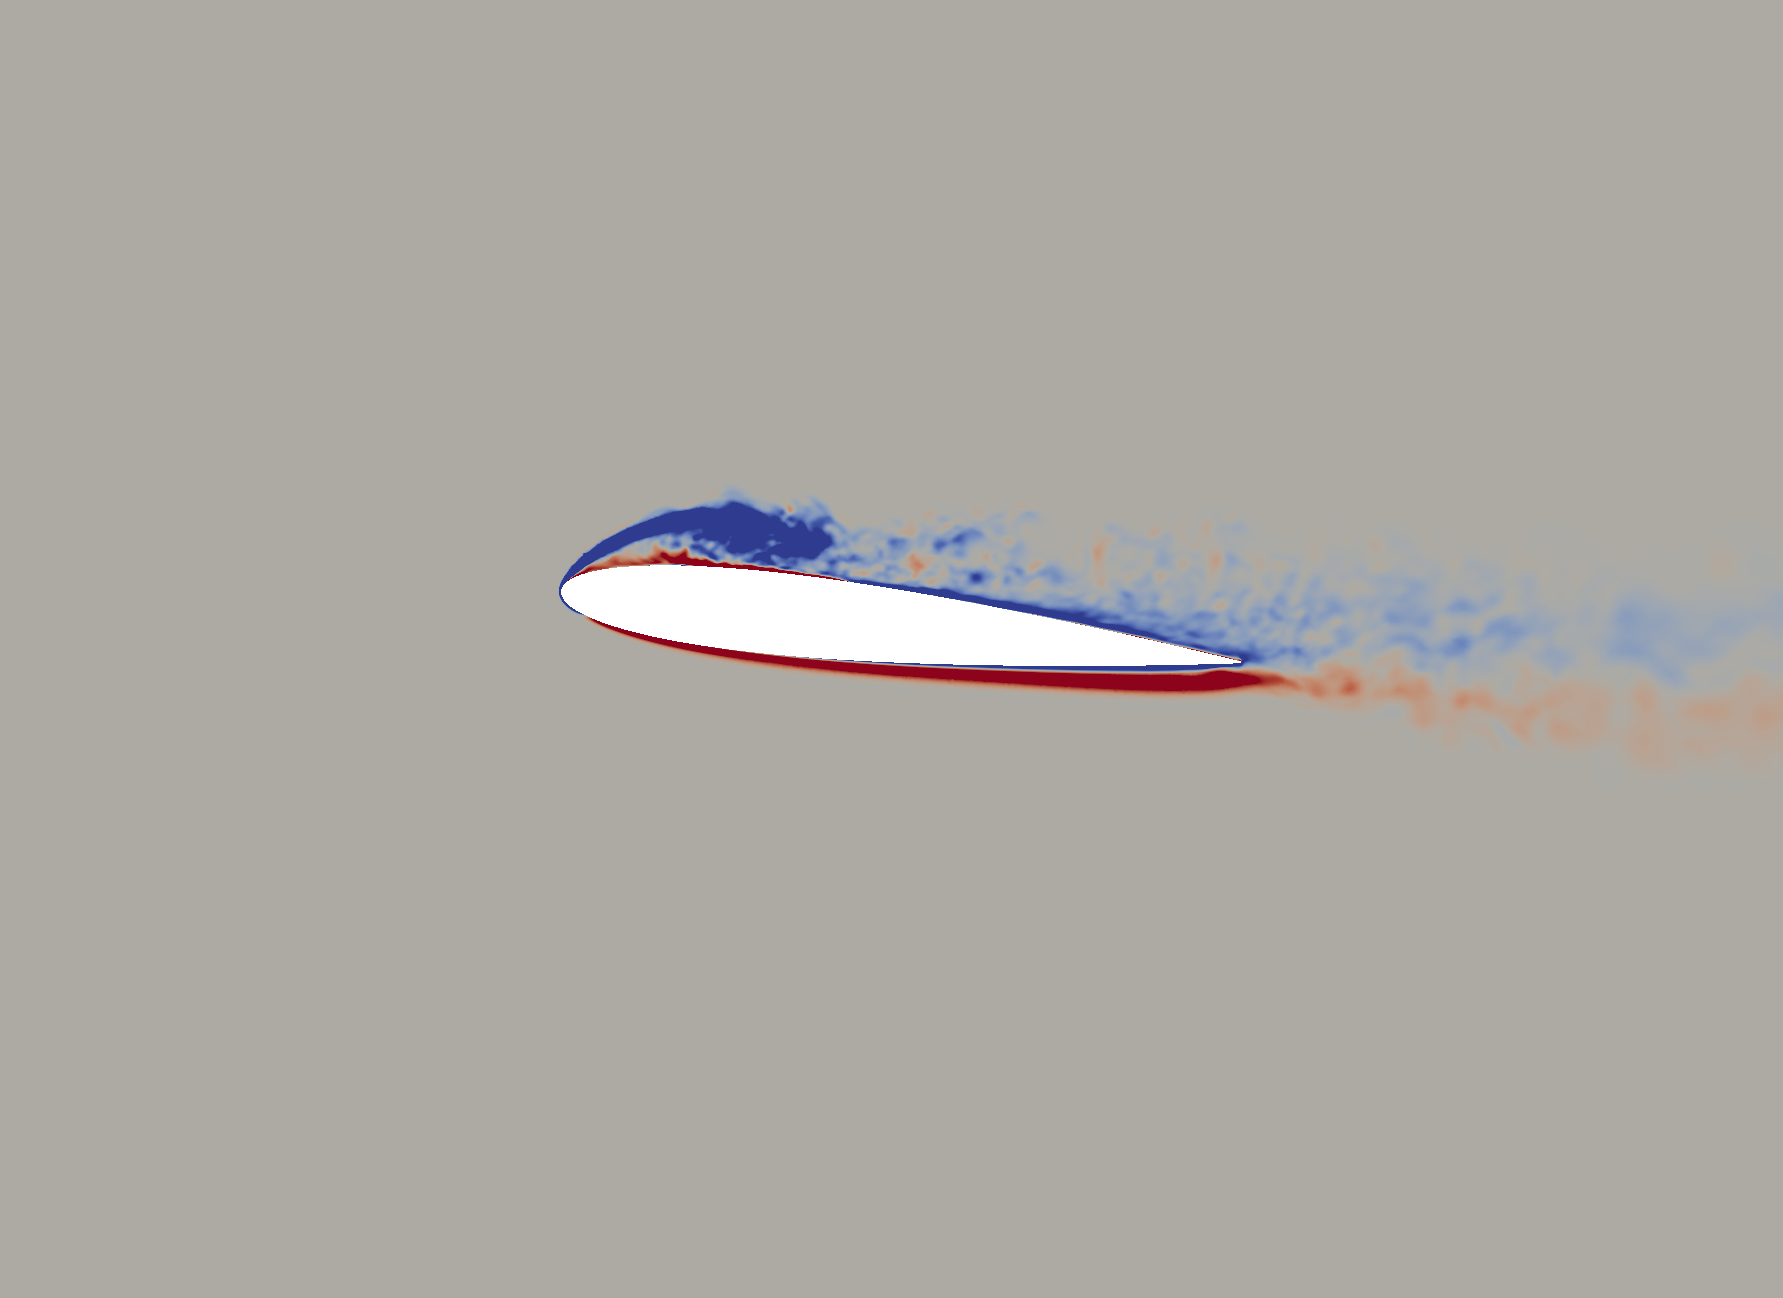
\includegraphics[width=1\textwidth]{figures/Vorticity_plots/Re_40k_1pt0/phase_225.png}
		\caption{$Re=4e4$, $\psi$ = $225^\circ$, $\tilde{t}=0.625$}
		\label{fig:Re_40k_1pt0_phi225}
	\end{subfigure}
	\begin{subfigure}[b]{0.32\textwidth}
		\centering
		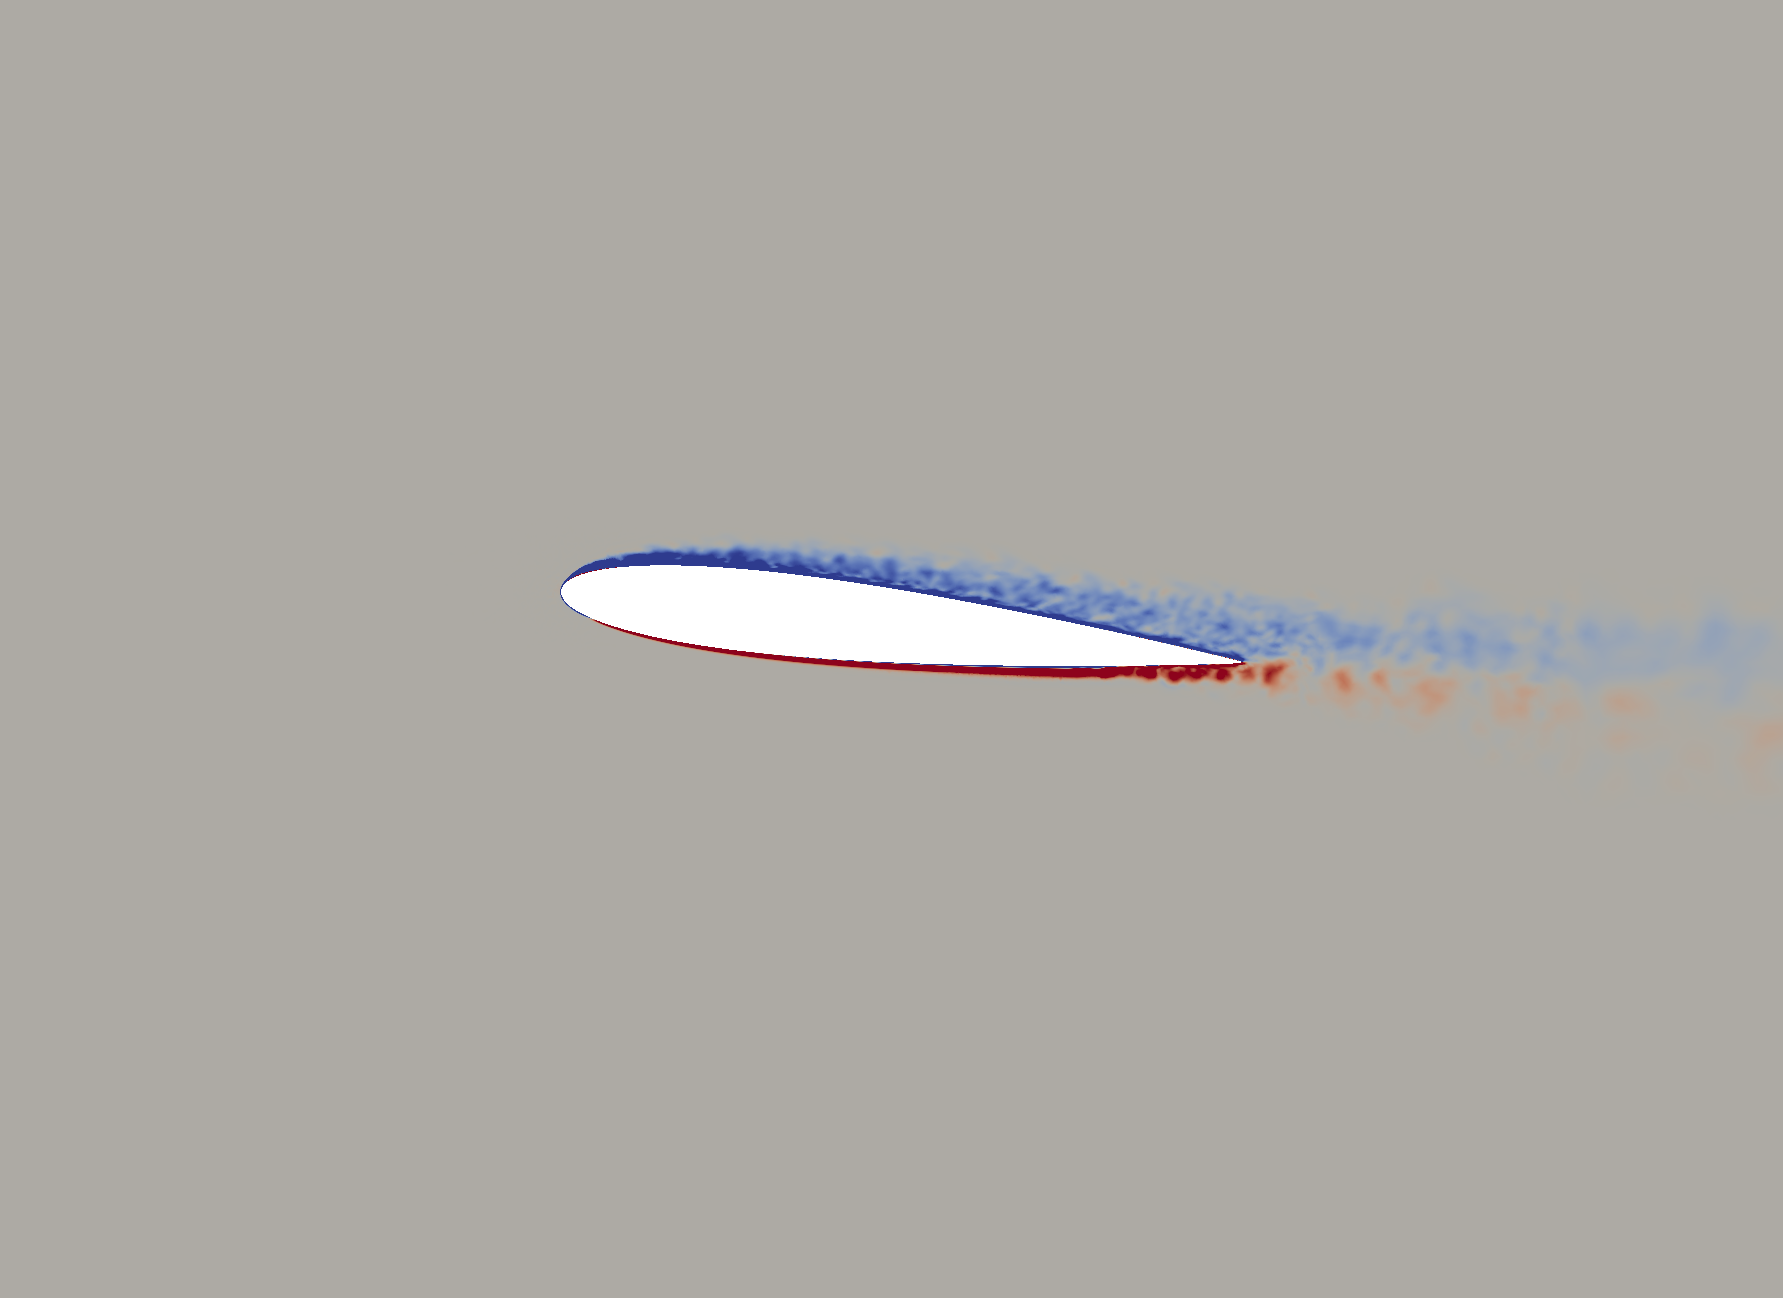
\includegraphics[width=1\textwidth]{figures/Vorticity_plots/Re_200k_1pt0/phase_225.png}
		\caption{$Re=2e5$, $\psi$ = $225^\circ$,  $\tilde{t}=0.625$}
		\label{fig:Re_200k_1pt0_phi225}
	\end{subfigure}
	\begin{subfigure}[b]{0.32\textwidth}
		\centering
		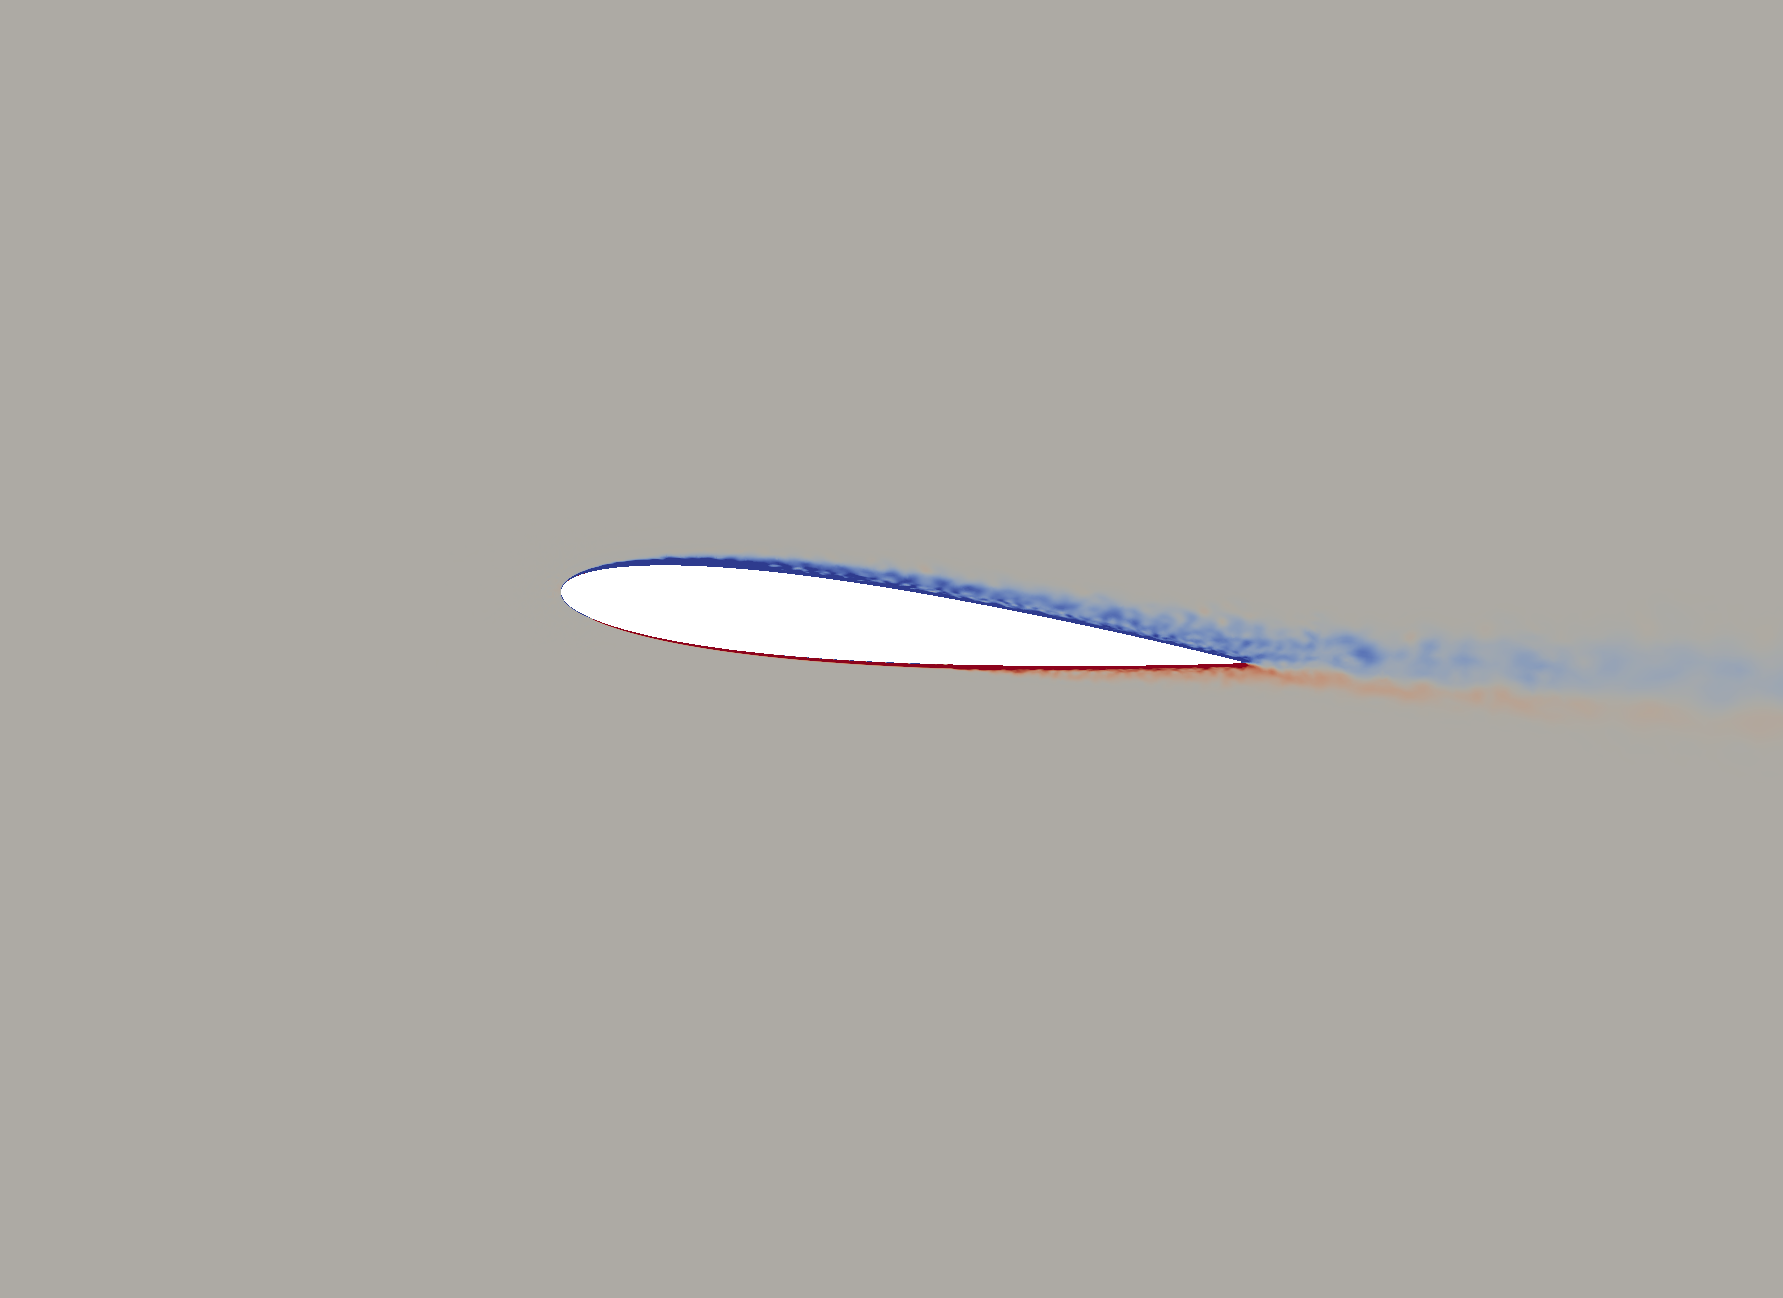
\includegraphics[width=1\textwidth]{figures/Vorticity_plots/Re_1m_1pt0/phase_225.png}
		\caption{$Re=1e6$, $\psi$ = $225^\circ$,  $\tilde{t}=0.625$}
		\label{fig:Re_1m_1pt0_phi225}
	\end{subfigure}
	
	\begin{subfigure}[b]{0.32\textwidth}
		\centering
		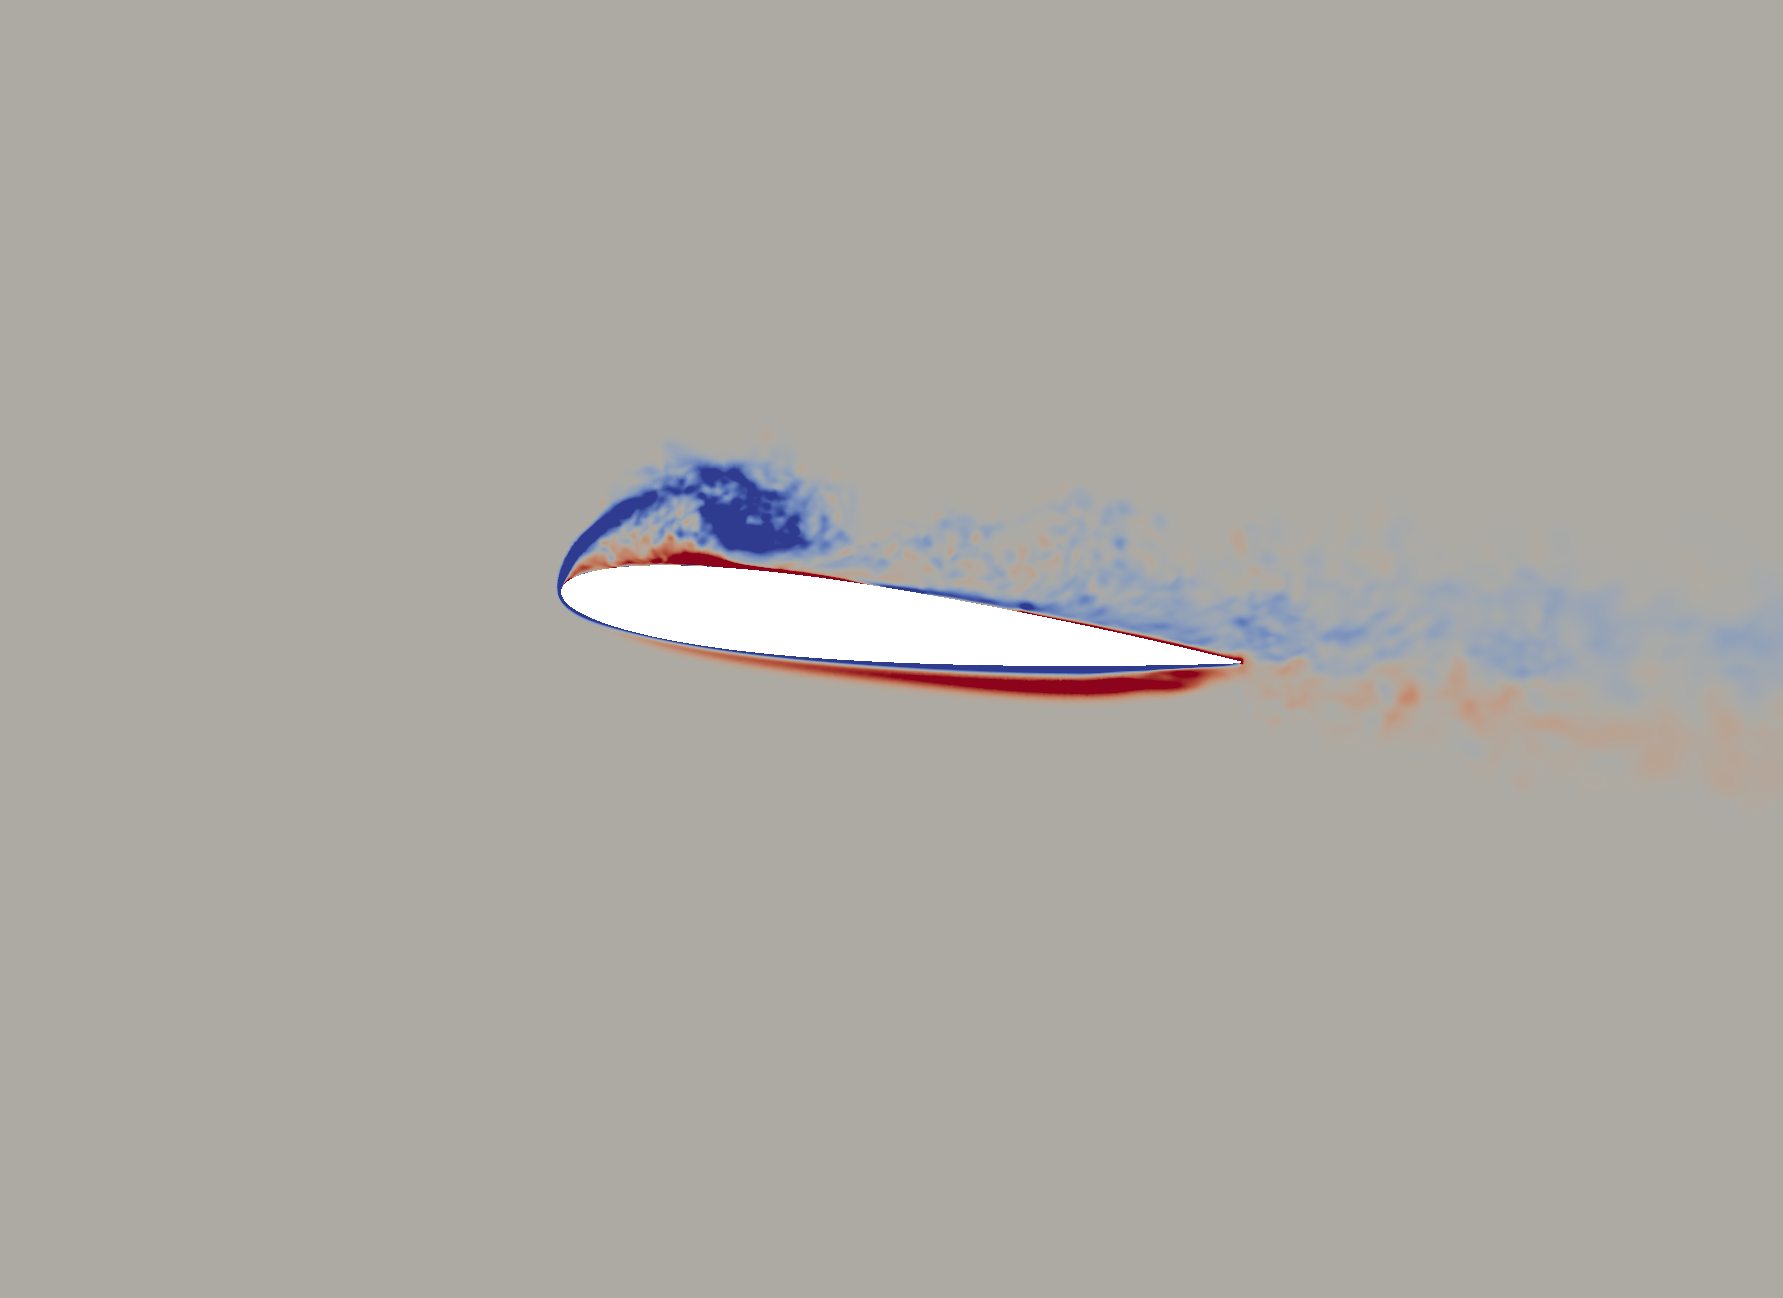
\includegraphics[width=1\textwidth]{figures/Vorticity_plots/Re_40k_1pt0/phase_240.png}
		\caption{$Re=4e4$, $\psi$ = $240^\circ$, $\tilde{t}=0.667$}
		\label{fig:Re_40k_1pt0_phi240}
	\end{subfigure}
	\begin{subfigure}[b]{0.32\textwidth}
		\centering
		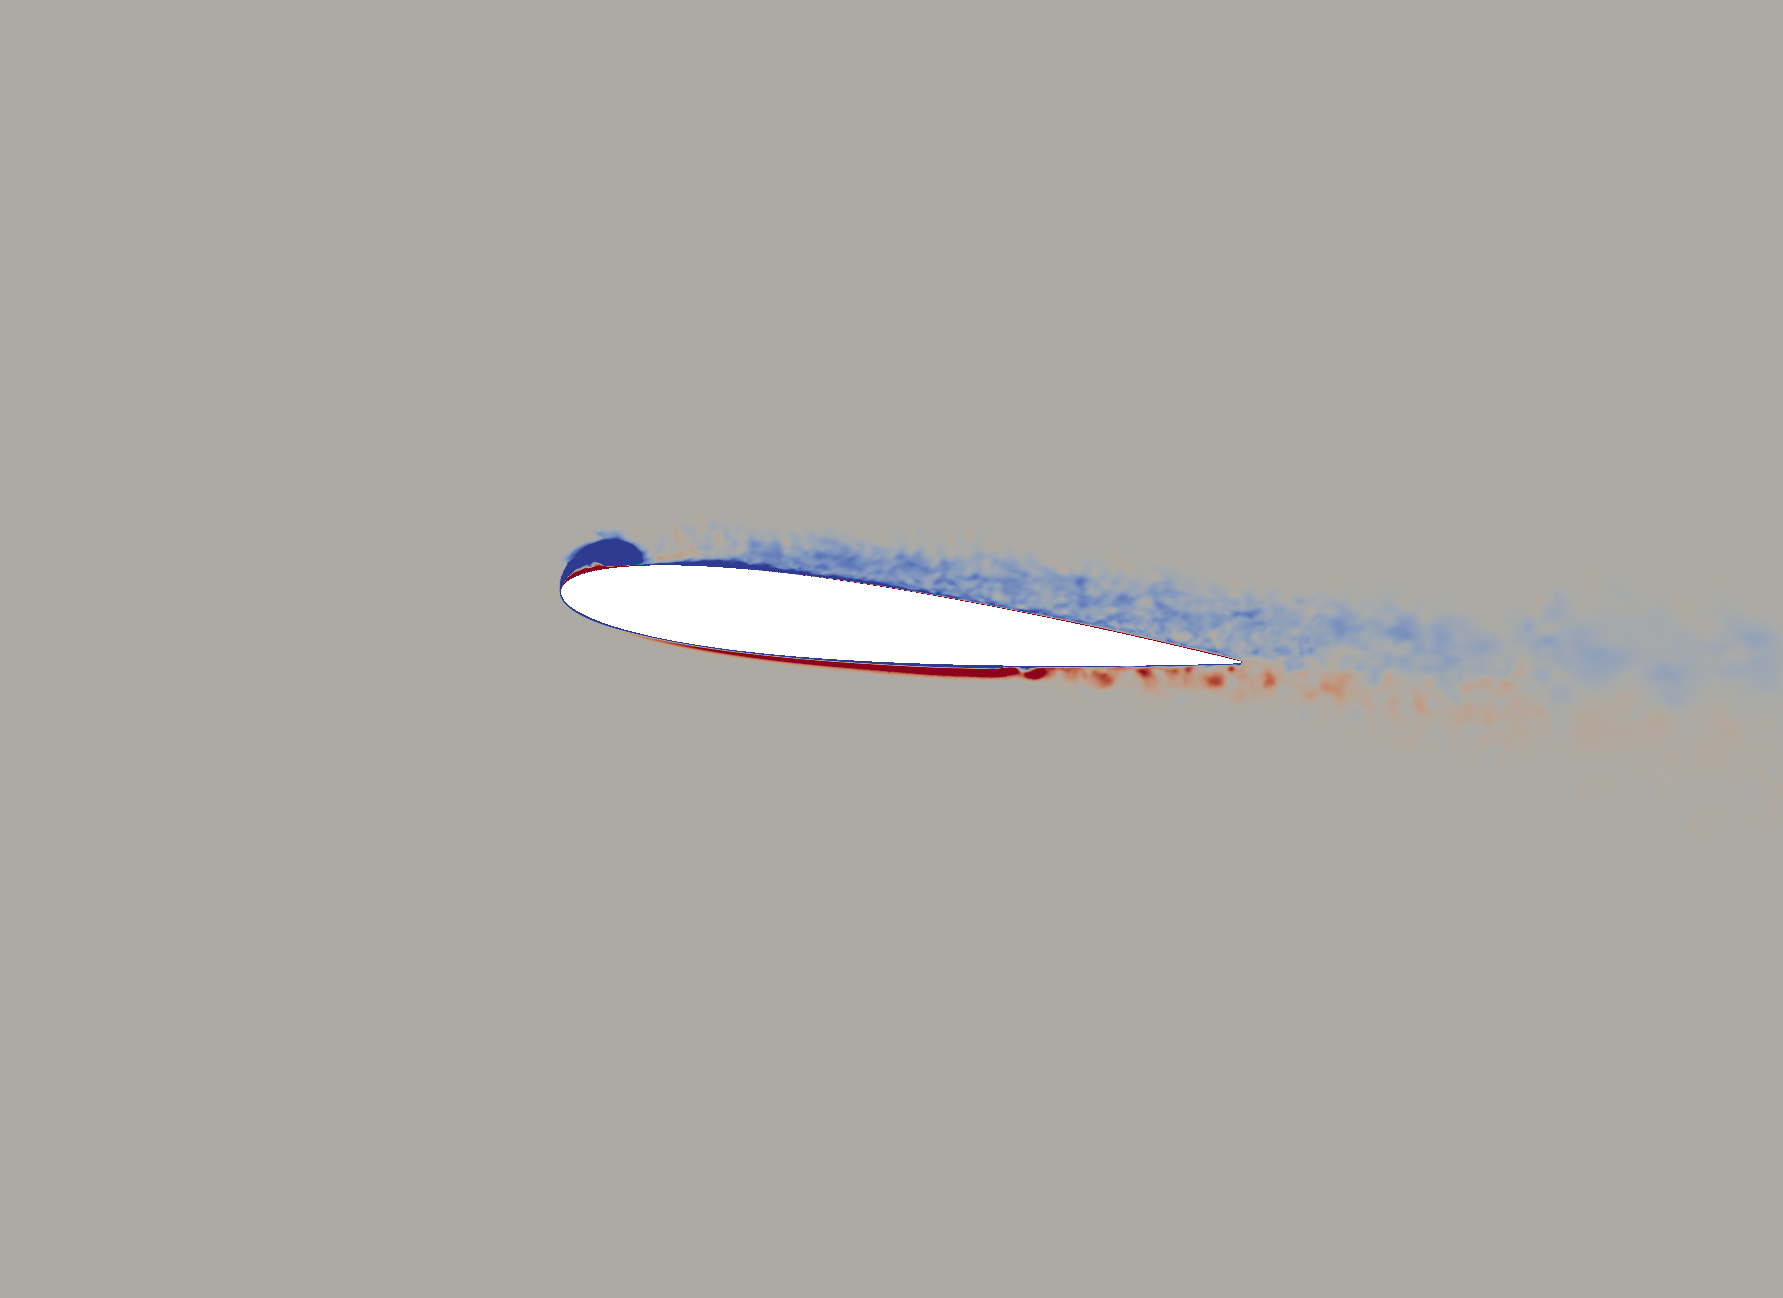
\includegraphics[width=1\textwidth]{figures/Vorticity_plots/Re_200k_1pt0/phase_240.png}
		\caption{$Re=2e5$, $\psi$ = $240^\circ$, $\tilde{t}=0.667$}
		\label{fig:Re_200k_1pt0_phi240}
	\end{subfigure}
	\begin{subfigure}[b]{0.32\textwidth}
		\centering
		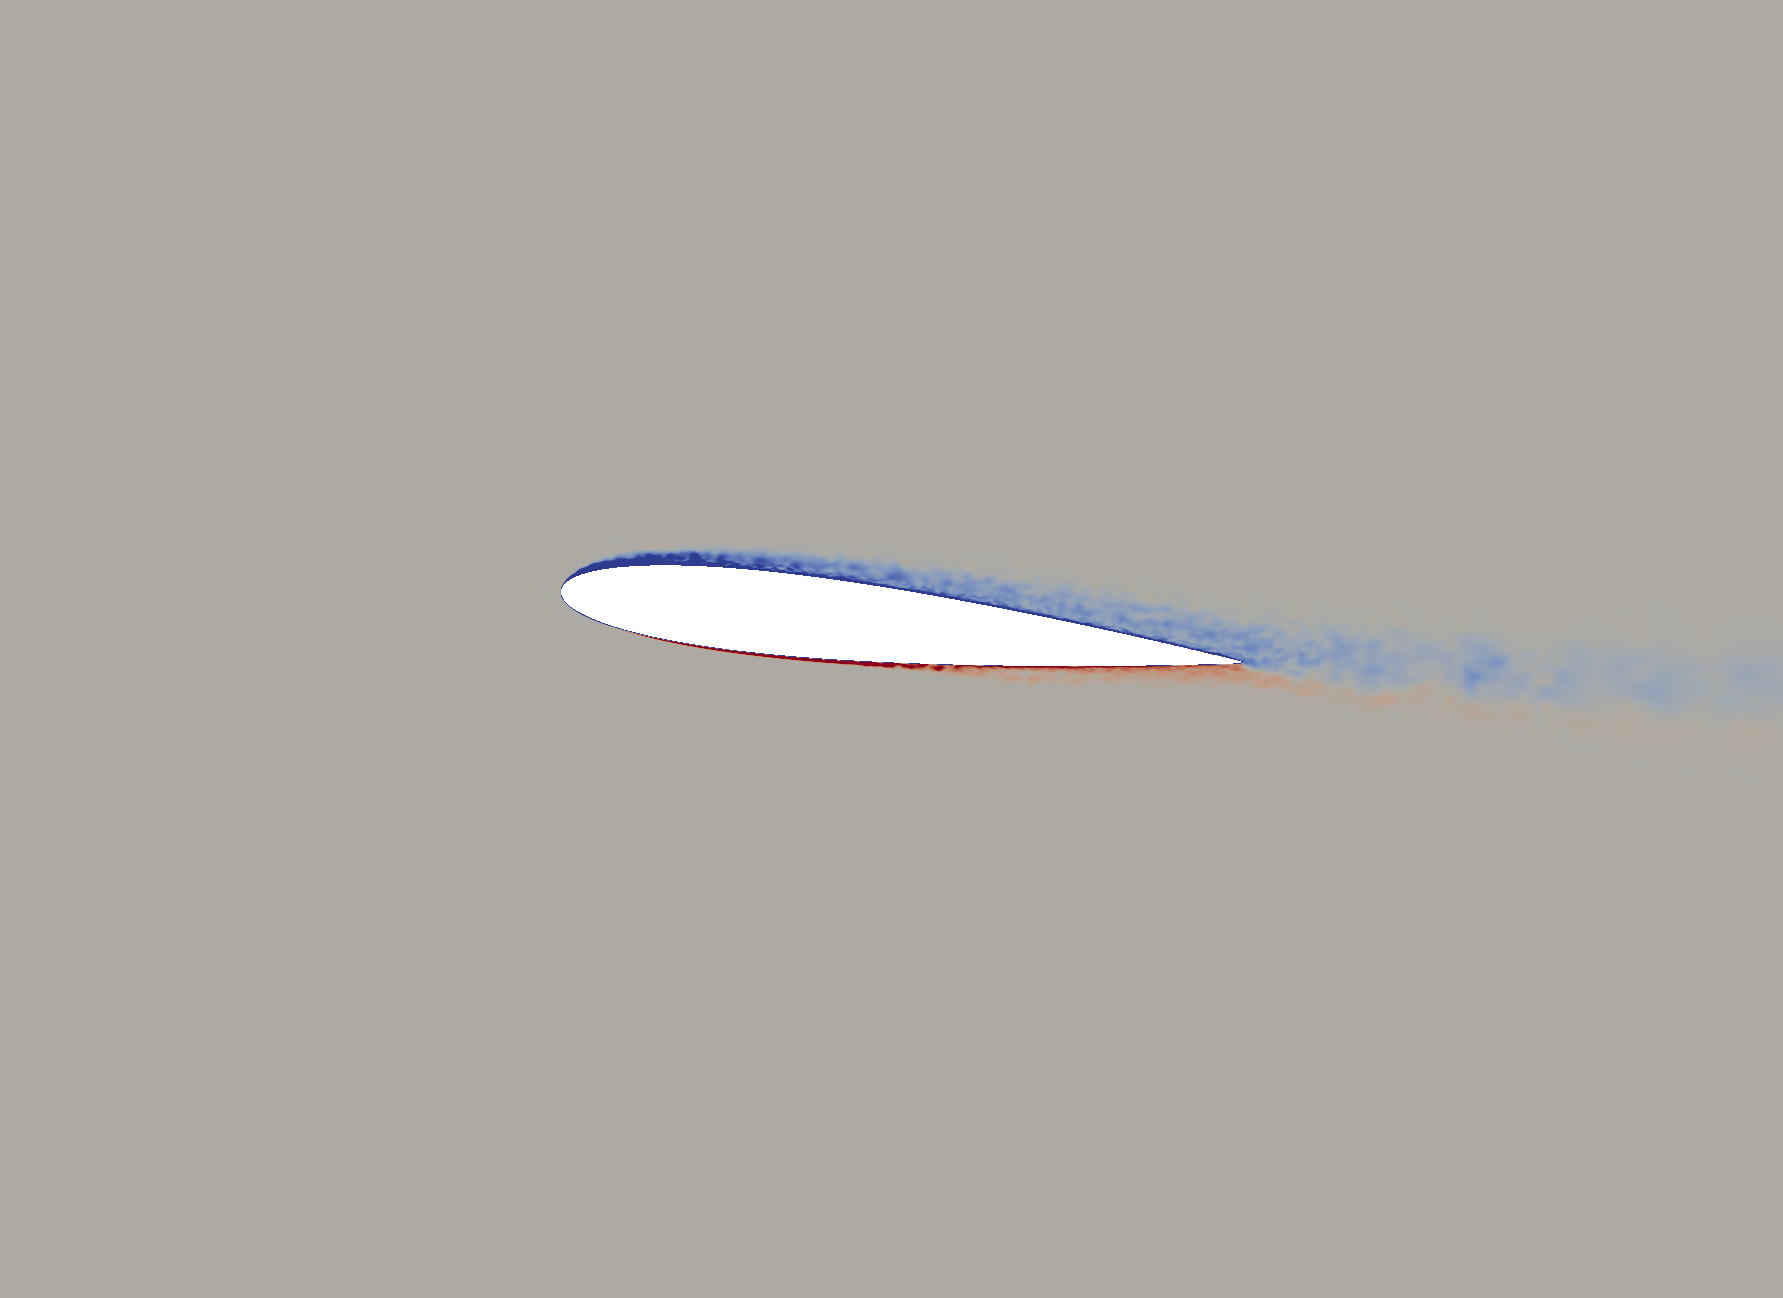
\includegraphics[width=1\textwidth]{figures/Vorticity_plots/Re_1m_1pt0/phase_240.png}
		\caption{$Re=1e6$, $\psi$ = $240^\circ$, $\tilde{t}=0.667$}
		\label{fig:Re_1m_1pt0_phi240}
	\end{subfigure}
	
	\begin{subfigure}[b]{0.32\textwidth}
		\centering
		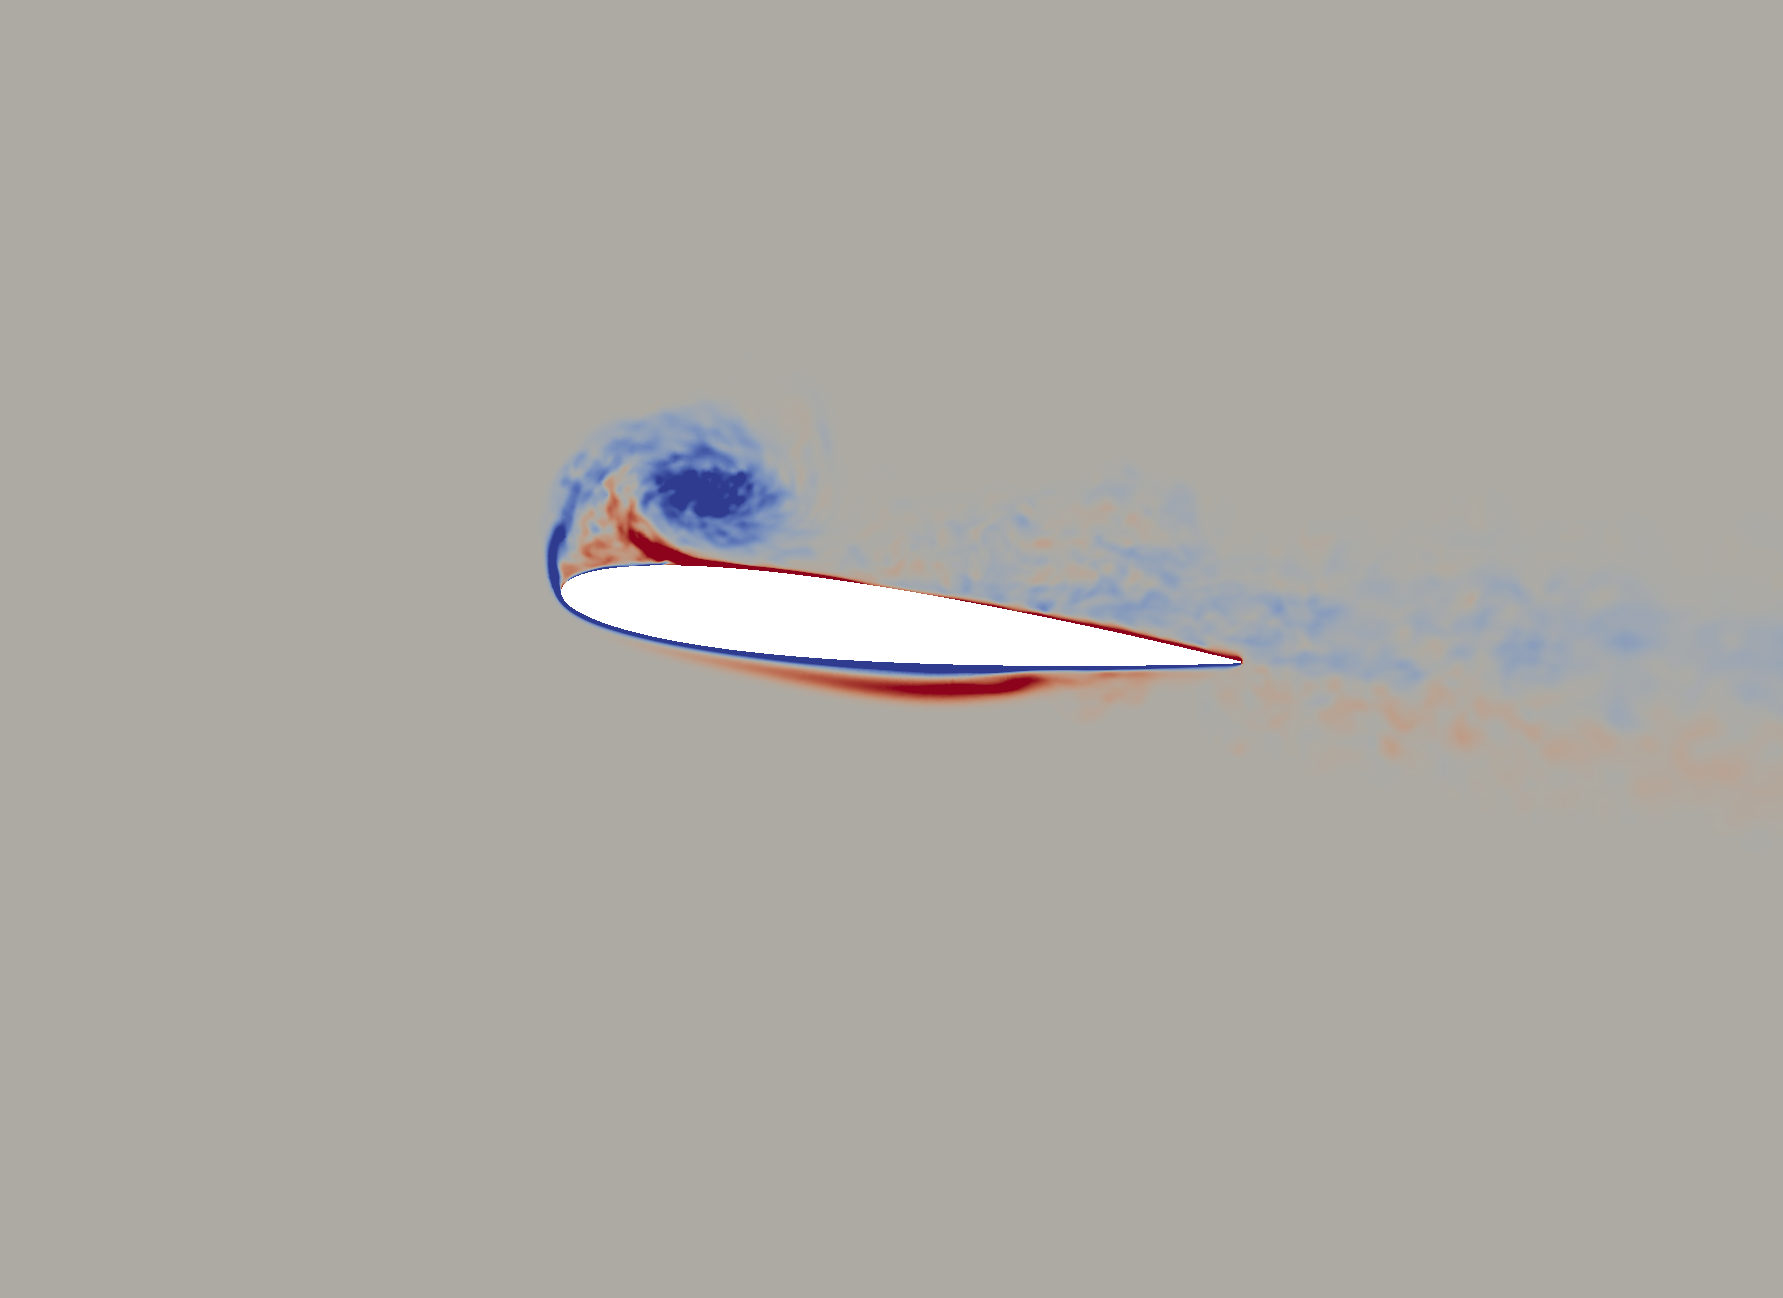
\includegraphics[width=1\textwidth]{figures/Vorticity_plots/Re_40k_1pt0/phase_255.png}
		\caption{$Re=4e4$, $\psi$ = $255^\circ$, $\tilde{t}=0.708$}
		\label{fig:Re_40k_1pt0_phi255}
	\end{subfigure}
	\begin{subfigure}[b]{0.32\textwidth}
		\centering
		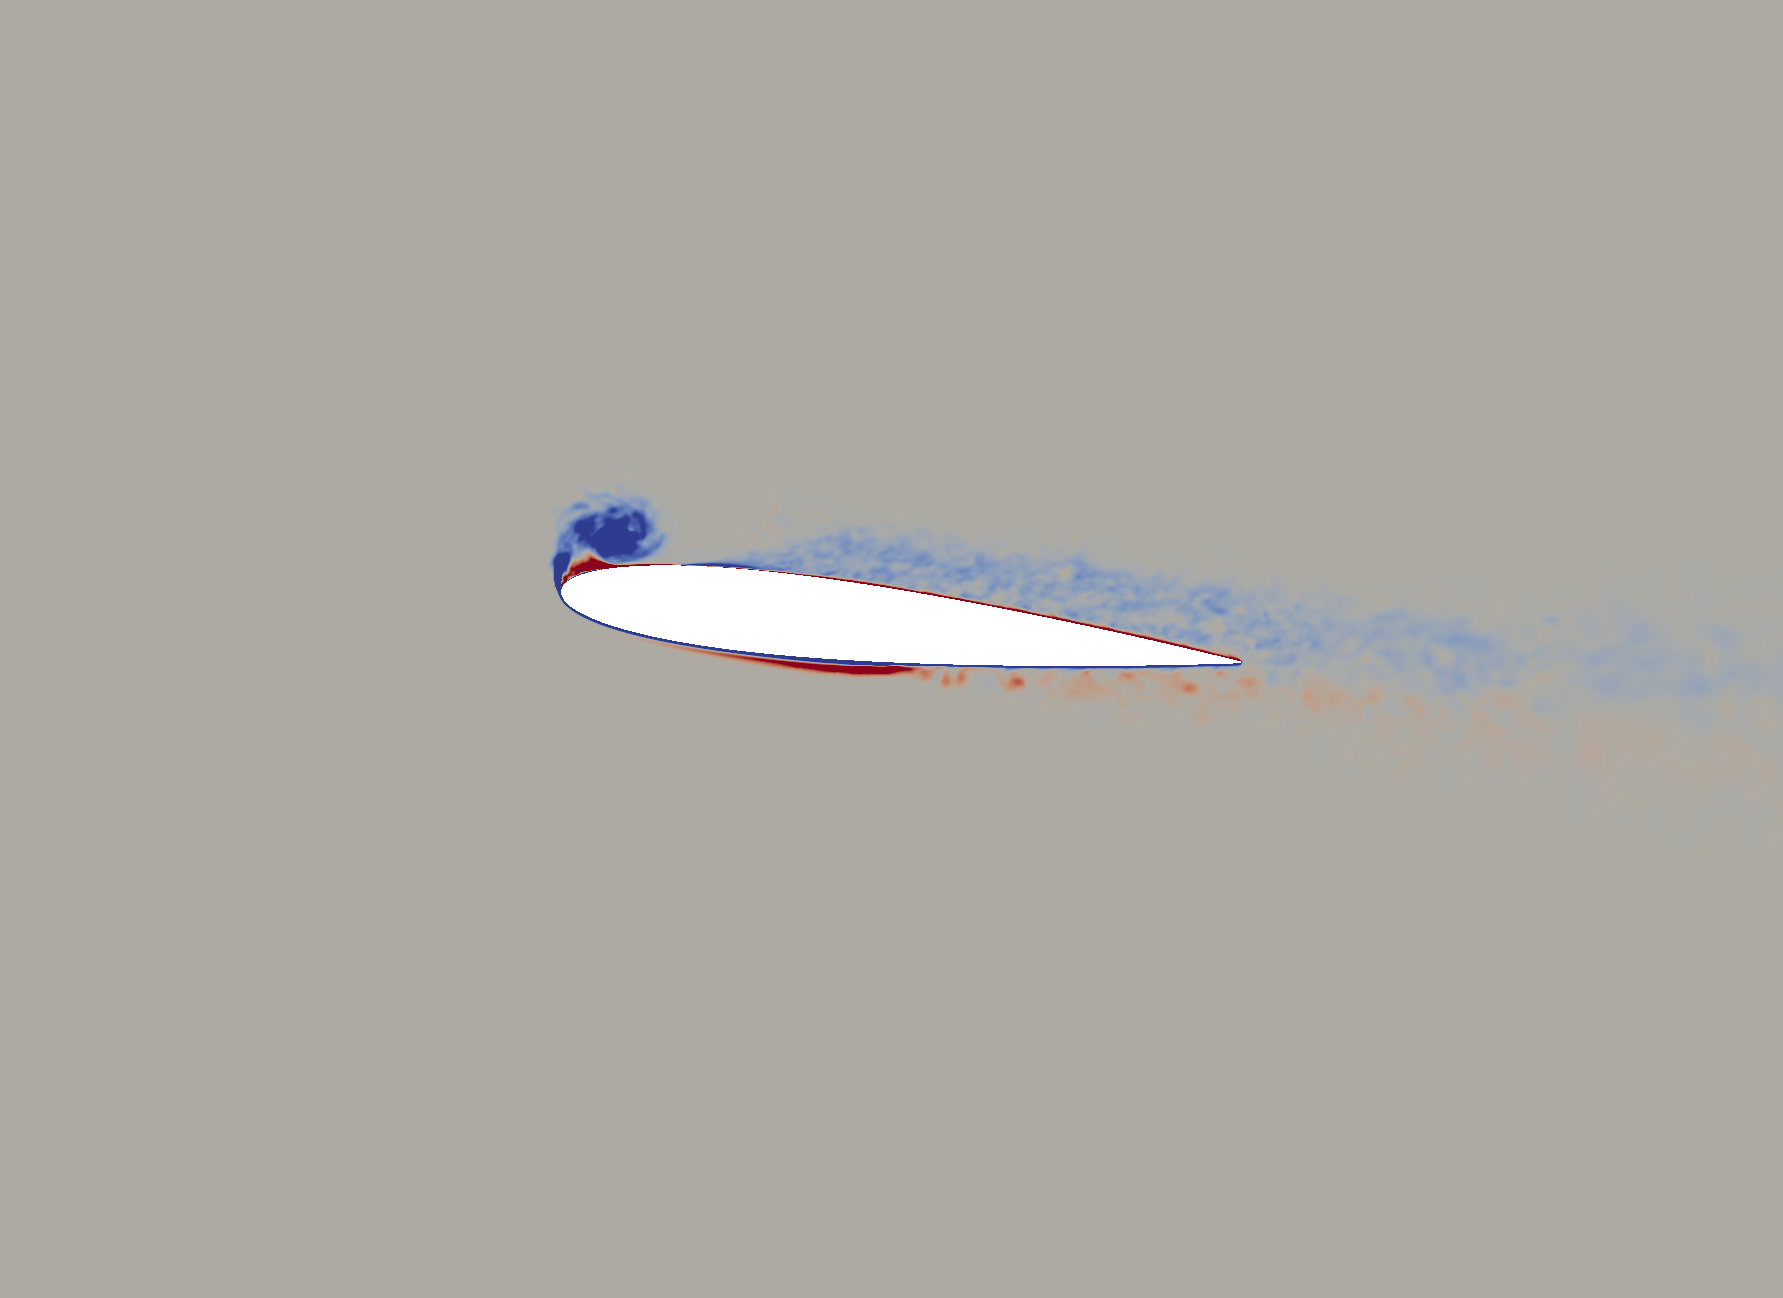
\includegraphics[width=1\textwidth]{figures/Vorticity_plots/Re_200k_1pt0/phase_255.png}
		\caption{$Re=2e5$, $\psi$ = $255^\circ$, $\tilde{t}=0.708$}
		\label{fig:Re_200k_1pt0_phi255}
	\end{subfigure}
	\begin{subfigure}[b]{0.32\textwidth}
		\centering
		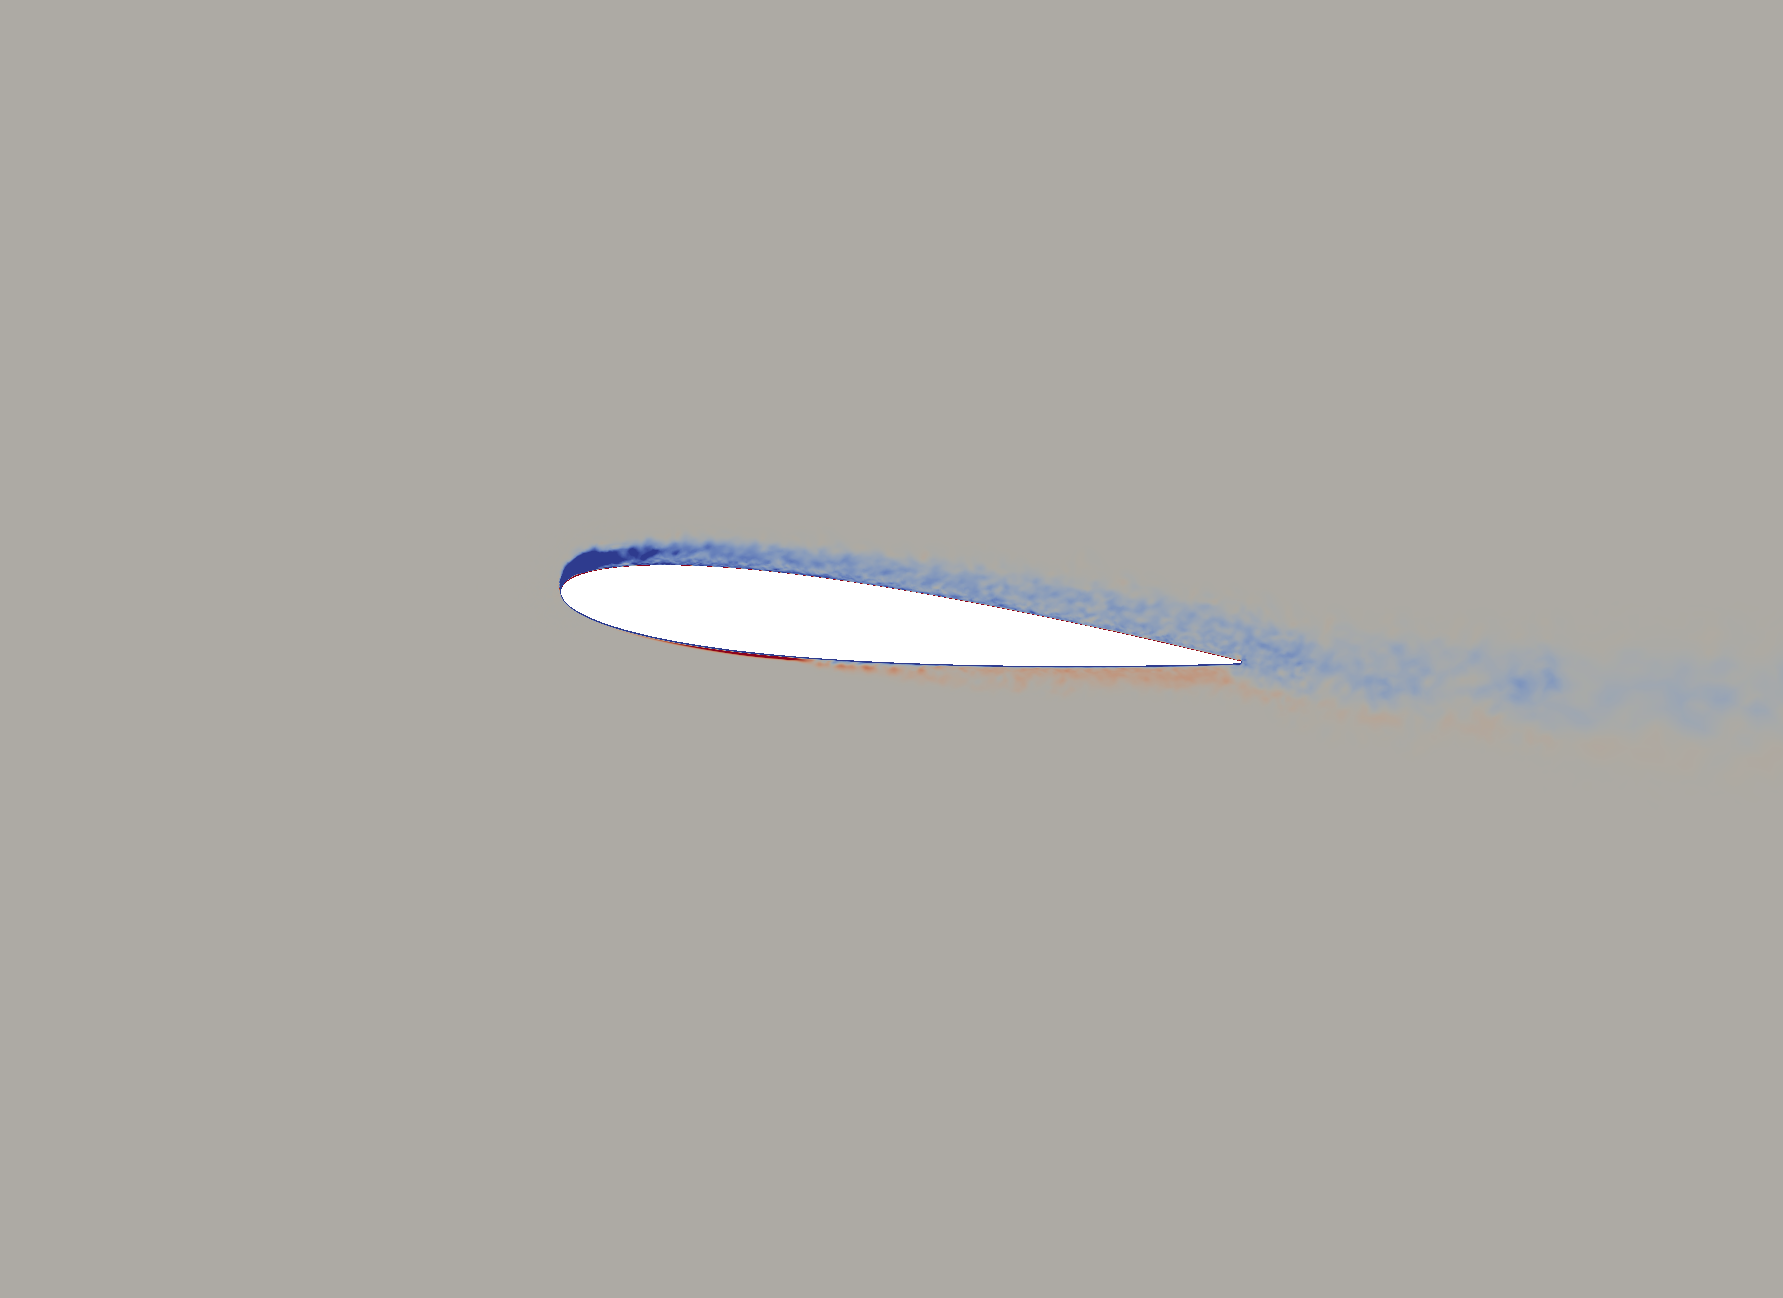
\includegraphics[width=1\textwidth]{figures/Vorticity_plots/Re_1m_1pt0/phase_255.png}
		\caption{$Re=1e6$, $\psi$ = $255^\circ$, $\tilde{t}=0.708$}
		\label{fig:Re_1m_1pt0_phi255}
	\end{subfigure}
	
	\caption{Spanwise vorticity at 8 different phases for $Re$=40,000 (left column), 200,000 (middle column) and 1,000,000 (right column) at $\mu_{sect}$ = 1.0}
	\label{fig:vortScreen_1pt0}
\end{figure}


\begin{figure}[H]\ContinuedFloat
	\centering
	\begin{subfigure}[b]{0.32\textwidth}
		\centering
		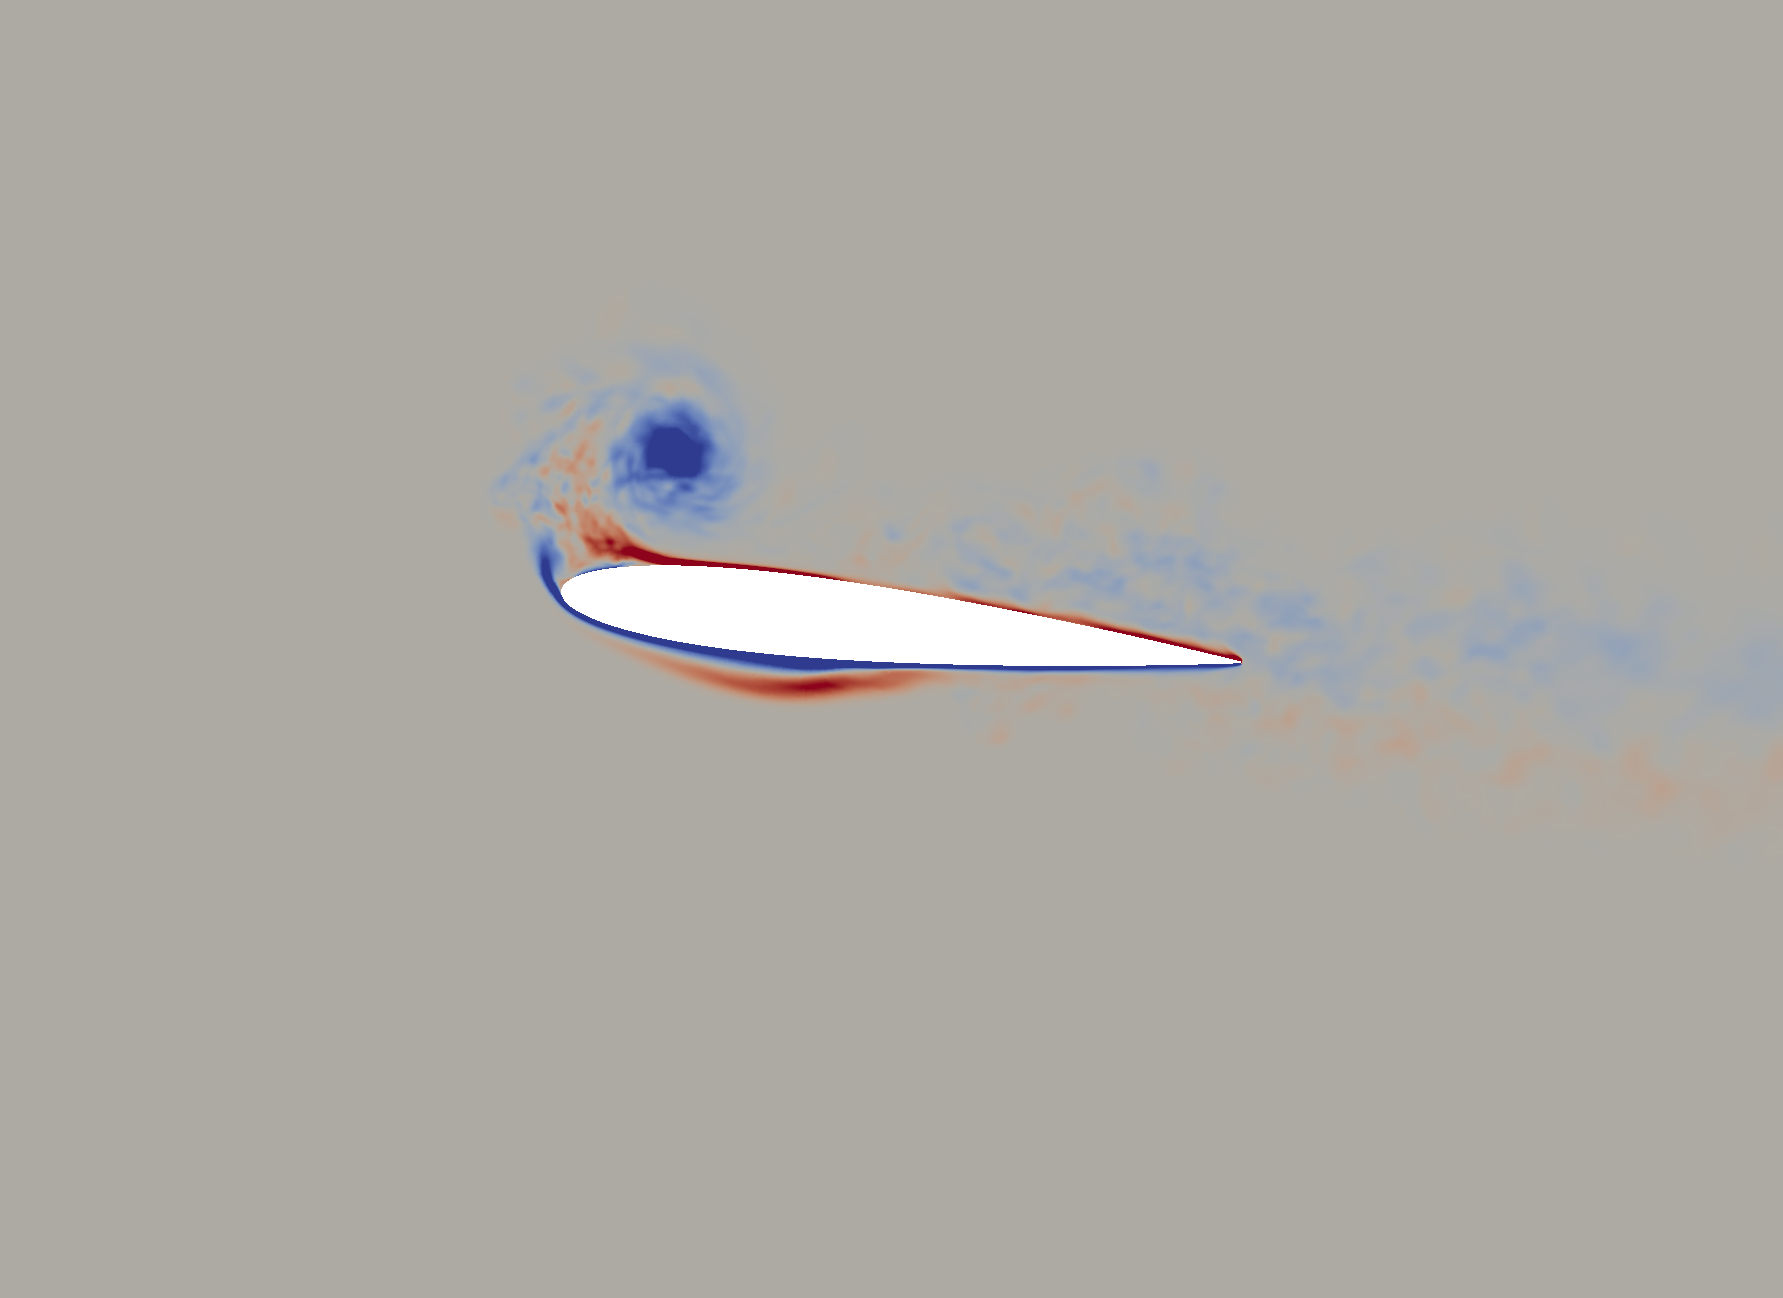
\includegraphics[width=1\textwidth]{figures/Vorticity_plots/Re_40k_1pt0/phase_270.png}
		\caption{$Re=4e4$, $\psi$ = $270^\circ$, $\tilde{t}=0.750$}
		\label{fig:Re_40k_1pt0_phi270}
	\end{subfigure}
	\begin{subfigure}[b]{0.32\textwidth}
		\centering
		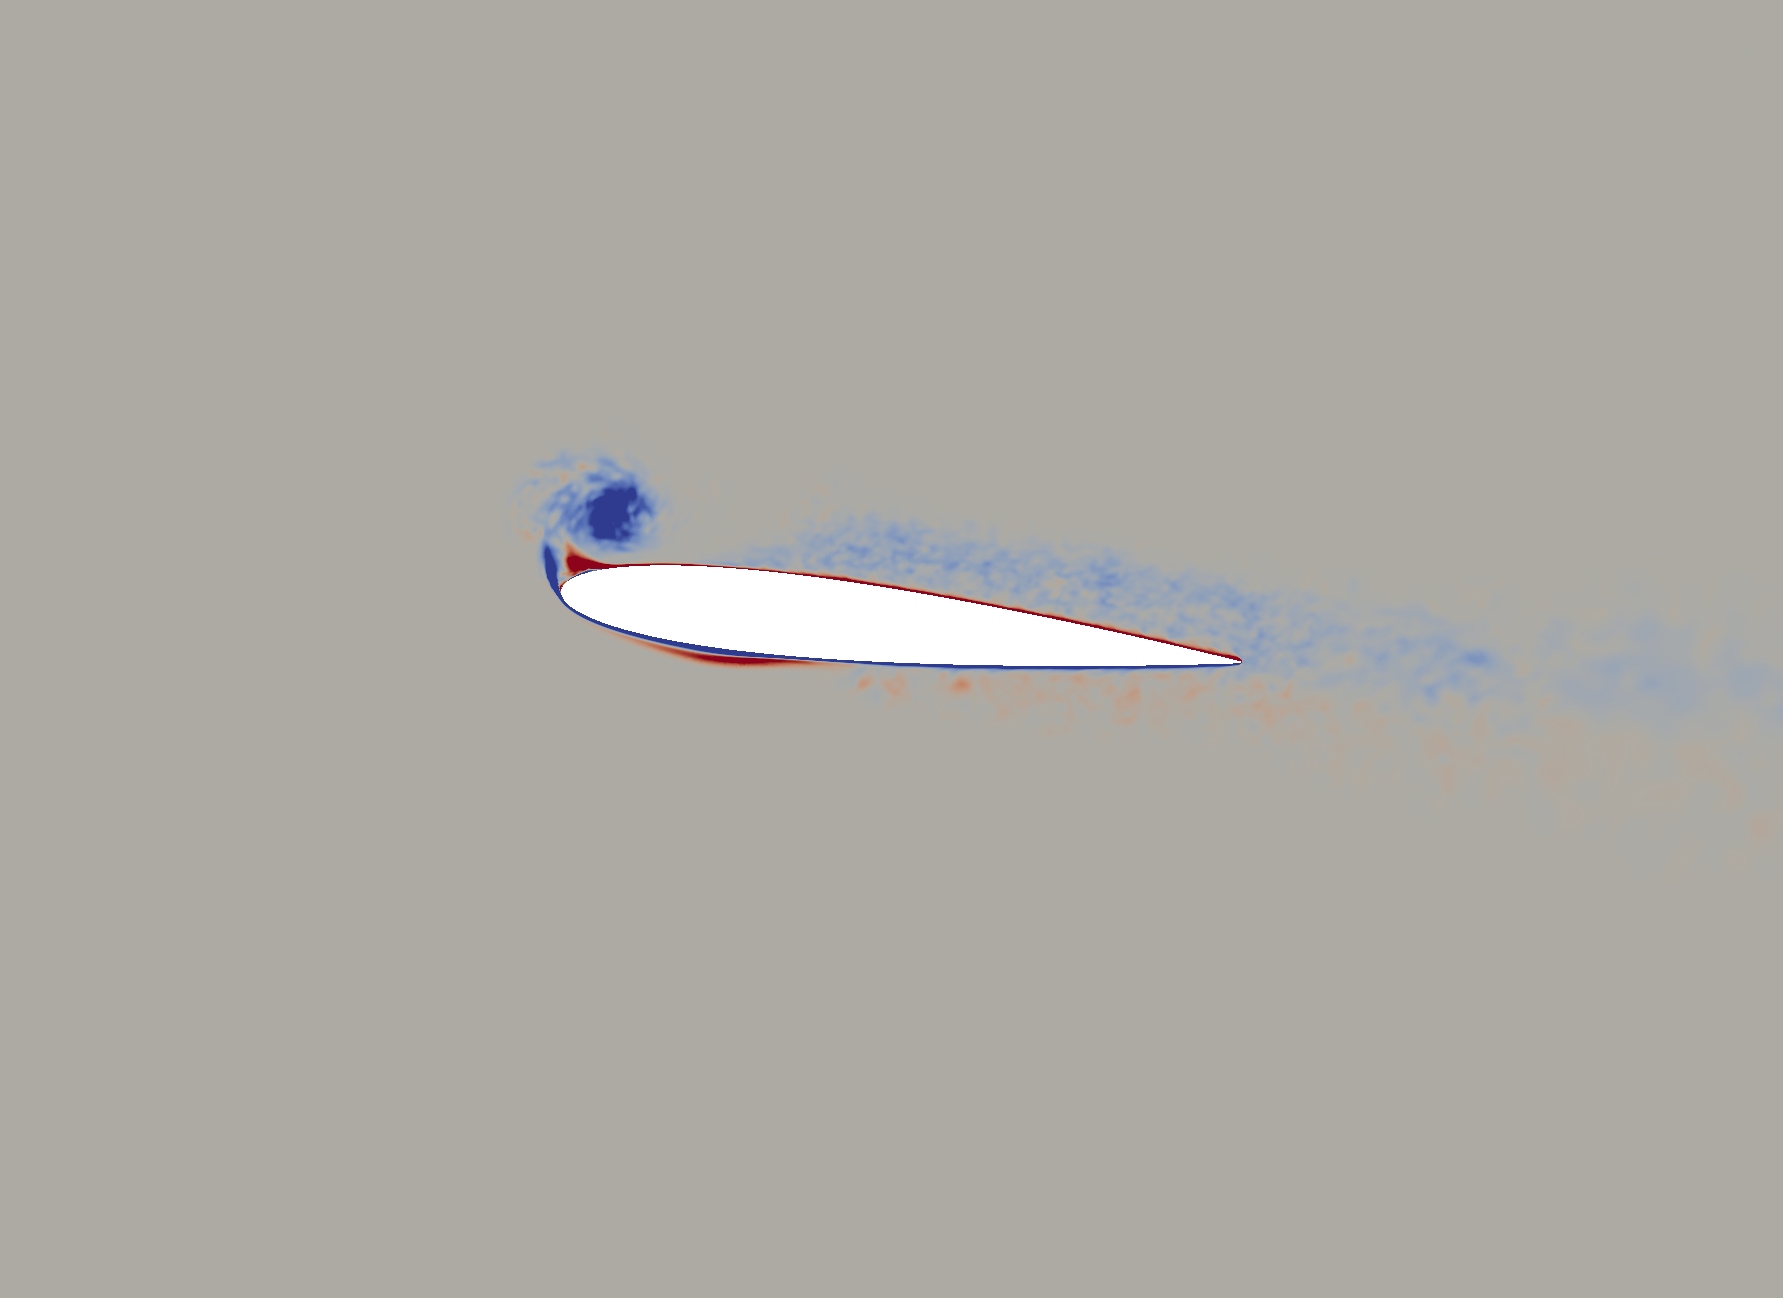
\includegraphics[width=1\textwidth]{figures/Vorticity_plots/Re_200k_1pt0/phase_270.png}
		\caption{$Re=2e5$, $\psi$ = $270^\circ$, $\tilde{t}=0.750$}
		\label{fig:Re_200k_1pt0_phi270}
	\end{subfigure}
	\begin{subfigure}[b]{0.32\textwidth}
		\centering
		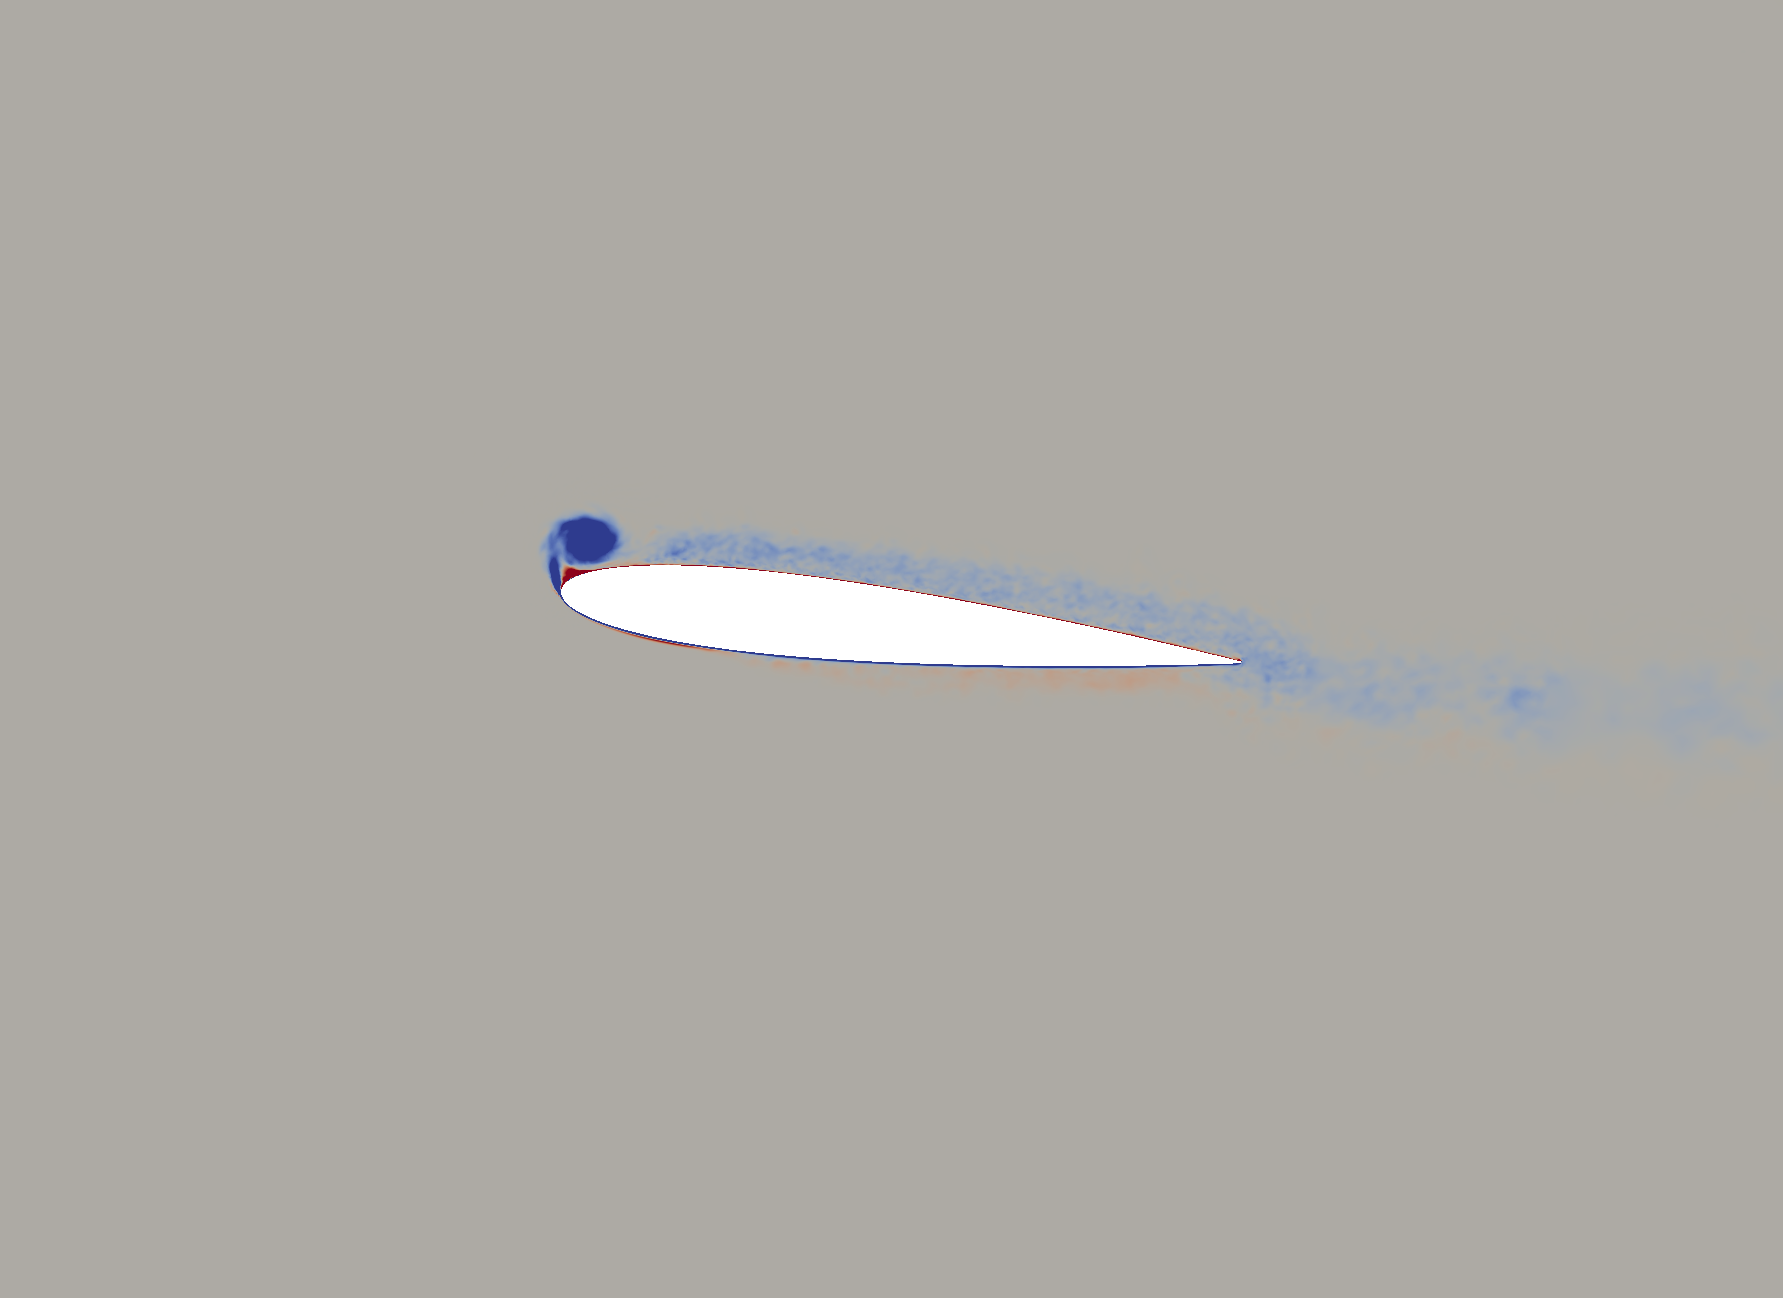
\includegraphics[width=1\textwidth]{figures/Vorticity_plots/Re_1m_1pt0/phase_270.png}
		\caption{$Re=1e6$, $\psi$ = $270^\circ$, $\tilde{t}=0.750$}
		\label{fig:Re_1m_1pt0_phi270}
	\end{subfigure}
	
	\begin{subfigure}[b]{0.32\textwidth}
		\centering
		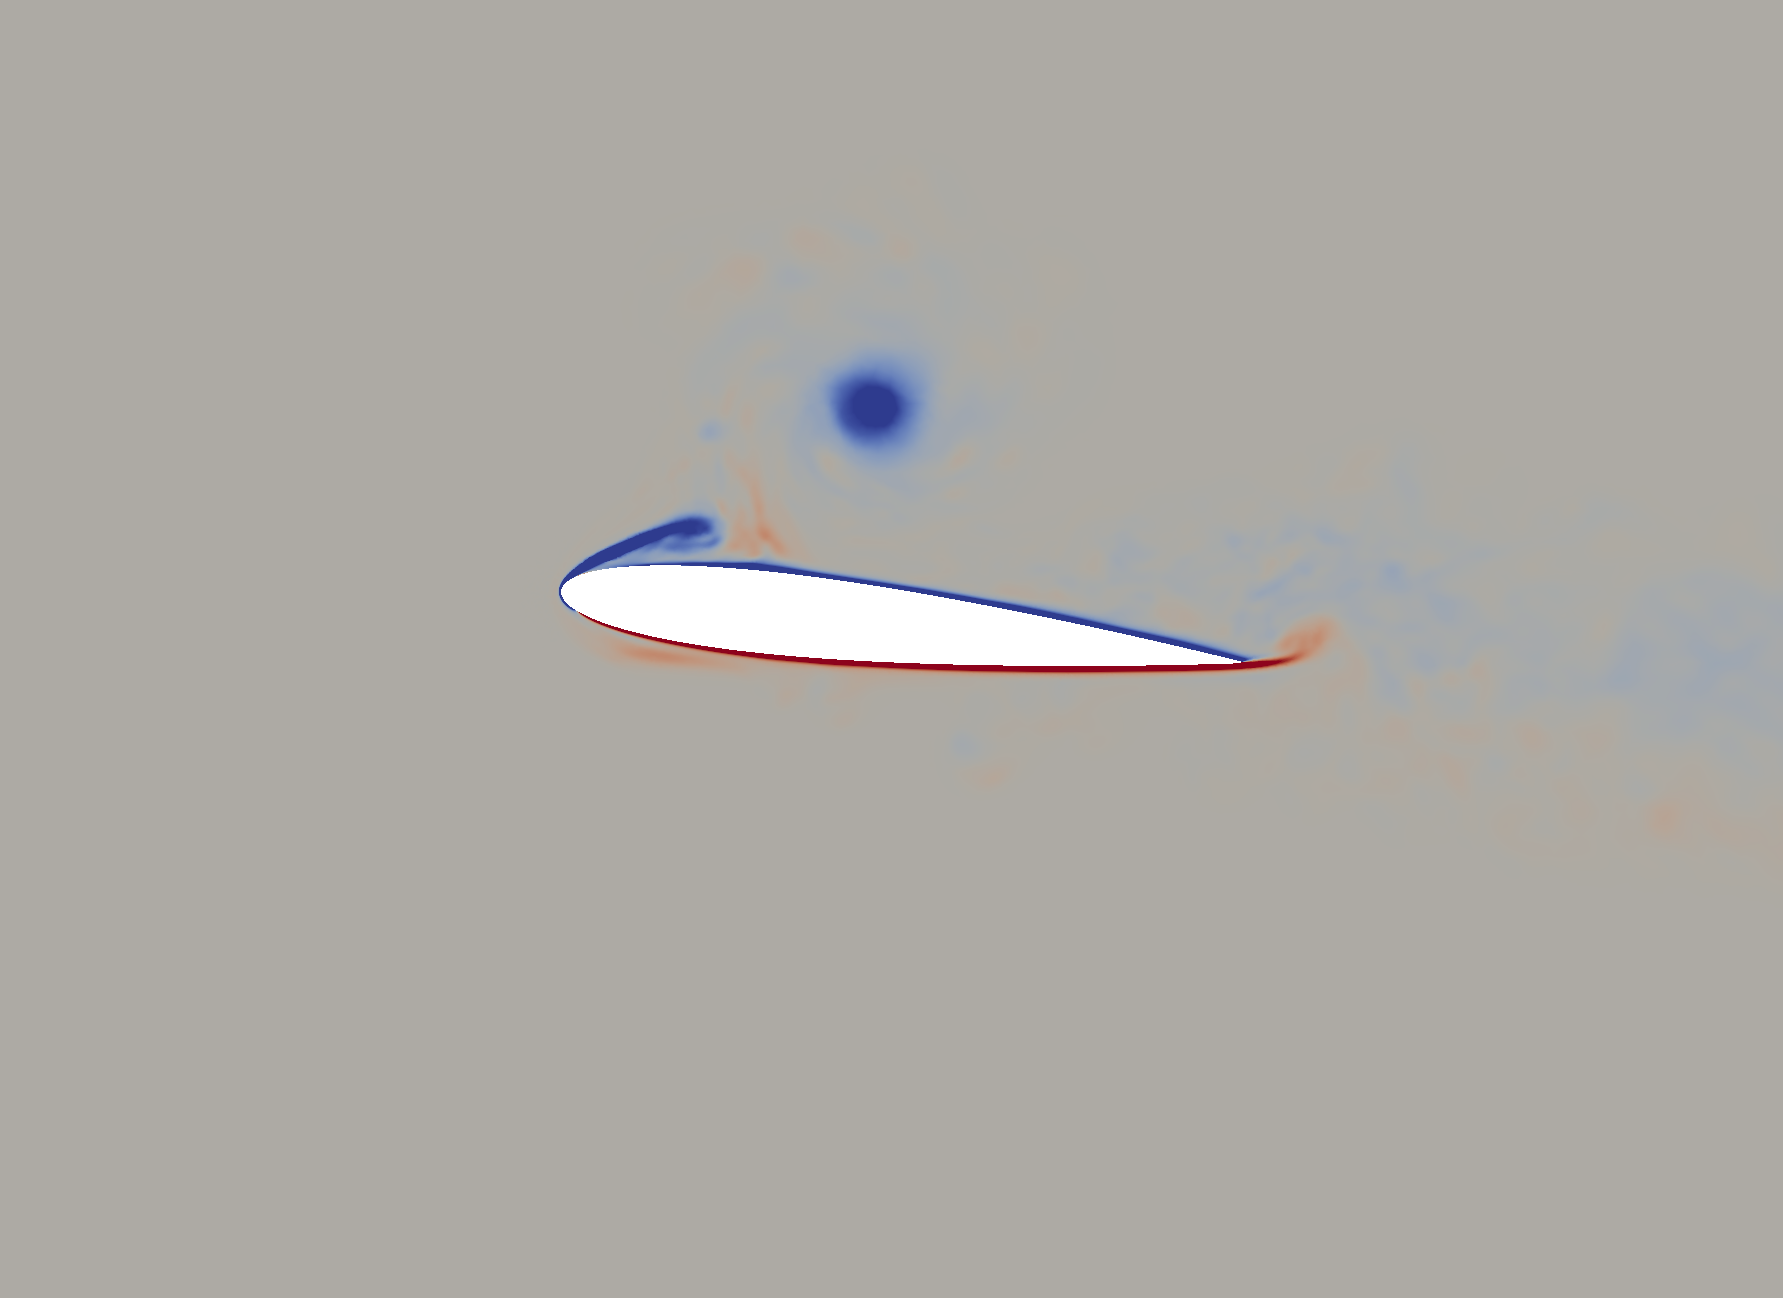
\includegraphics[width=1\textwidth]{figures/Vorticity_plots/Re_40k_1pt0/phase_315.png}
		\caption{$Re=4e4$, $\psi$ = $315^\circ$, $\tilde{t}=0.875$}
		\label{fig:Re_40k_1pt0_phi315}
	\end{subfigure}
	\begin{subfigure}[b]{0.32\textwidth}
		\centering
		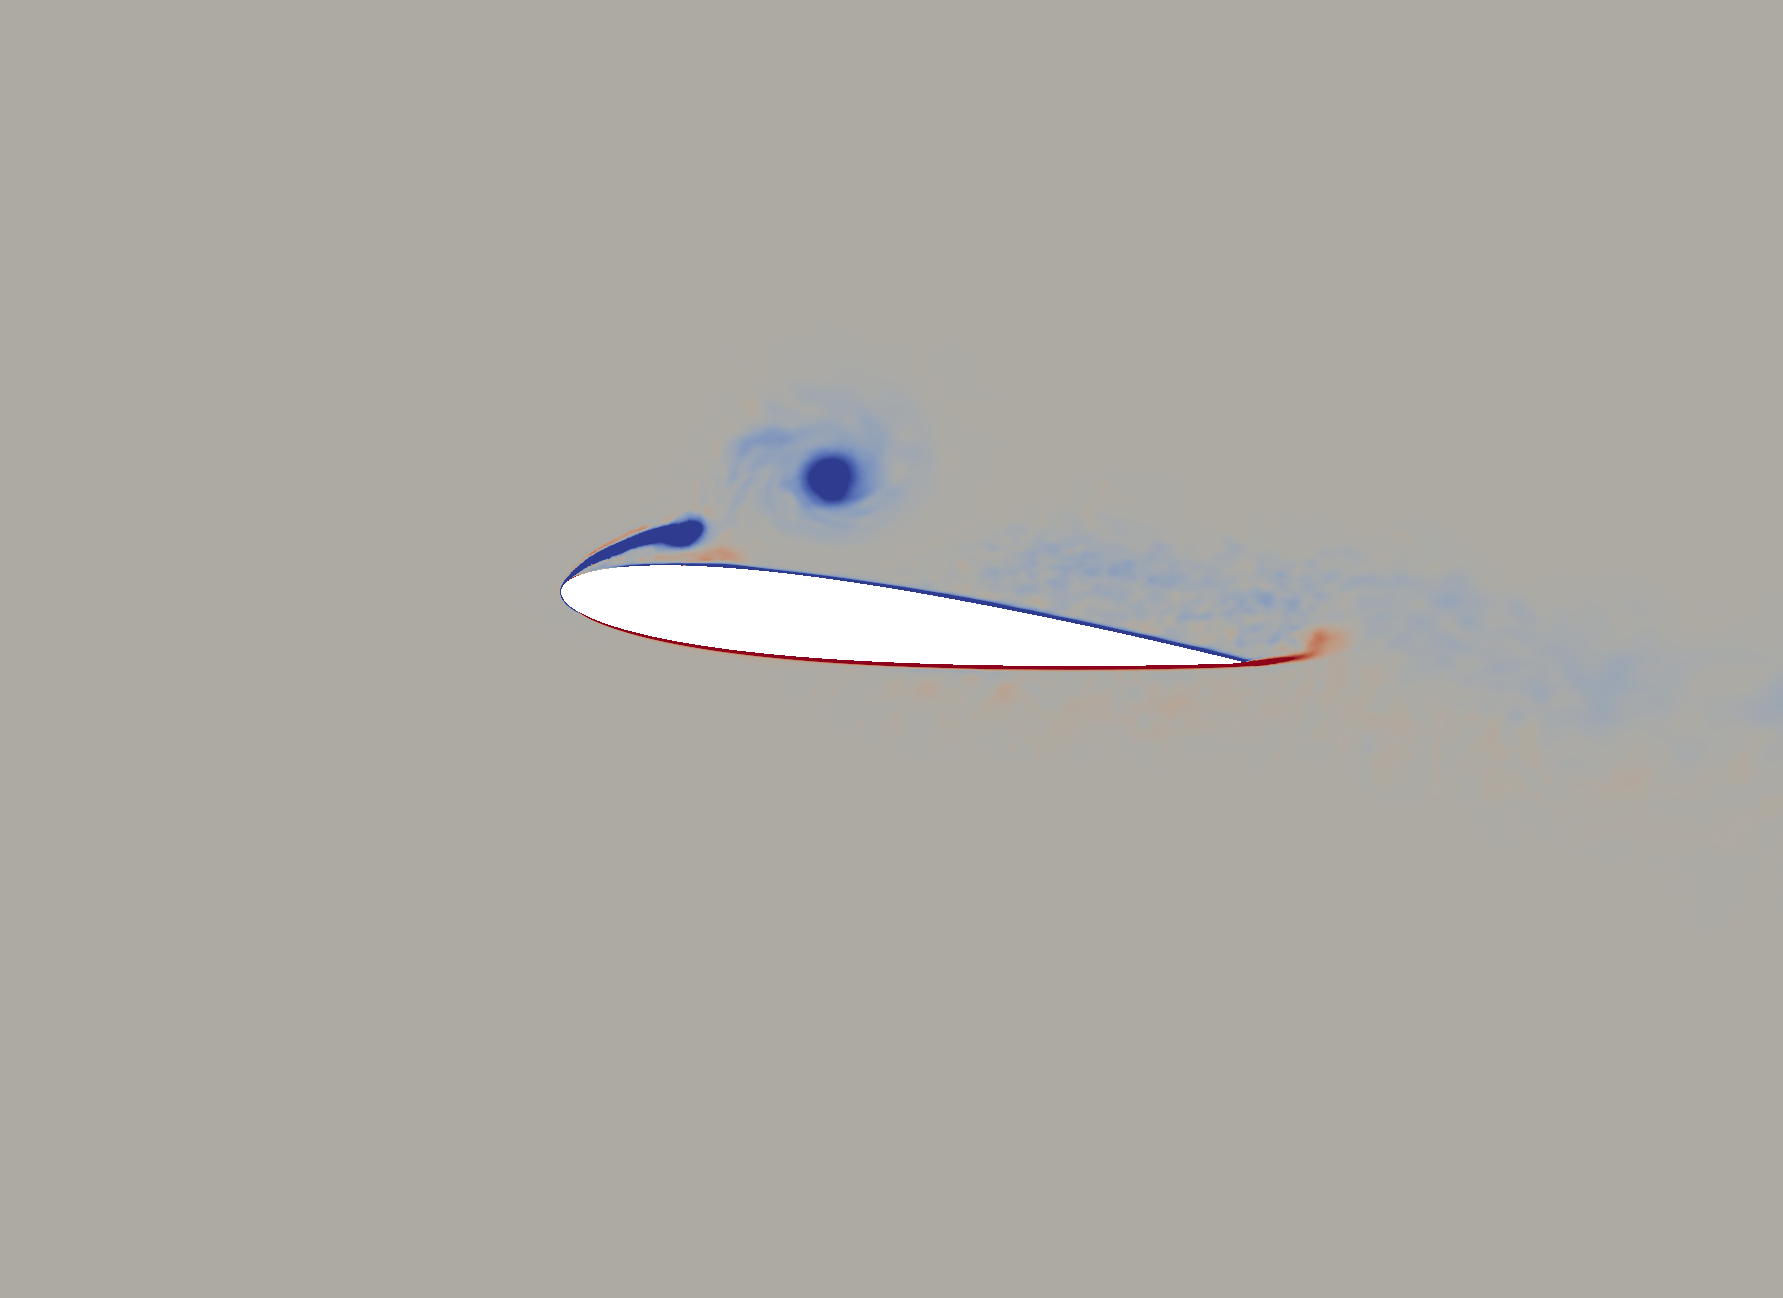
\includegraphics[width=1\textwidth]{figures/Vorticity_plots/Re_200k_1pt0/phase_315.png}
		\caption{$Re=2e5$, $\psi$ = $315^\circ$, $\tilde{t}=0.875$}
		\label{fig:Re_200k_1pt0_phi315}
	\end{subfigure}
	\begin{subfigure}[b]{0.32\textwidth}
		\centering
		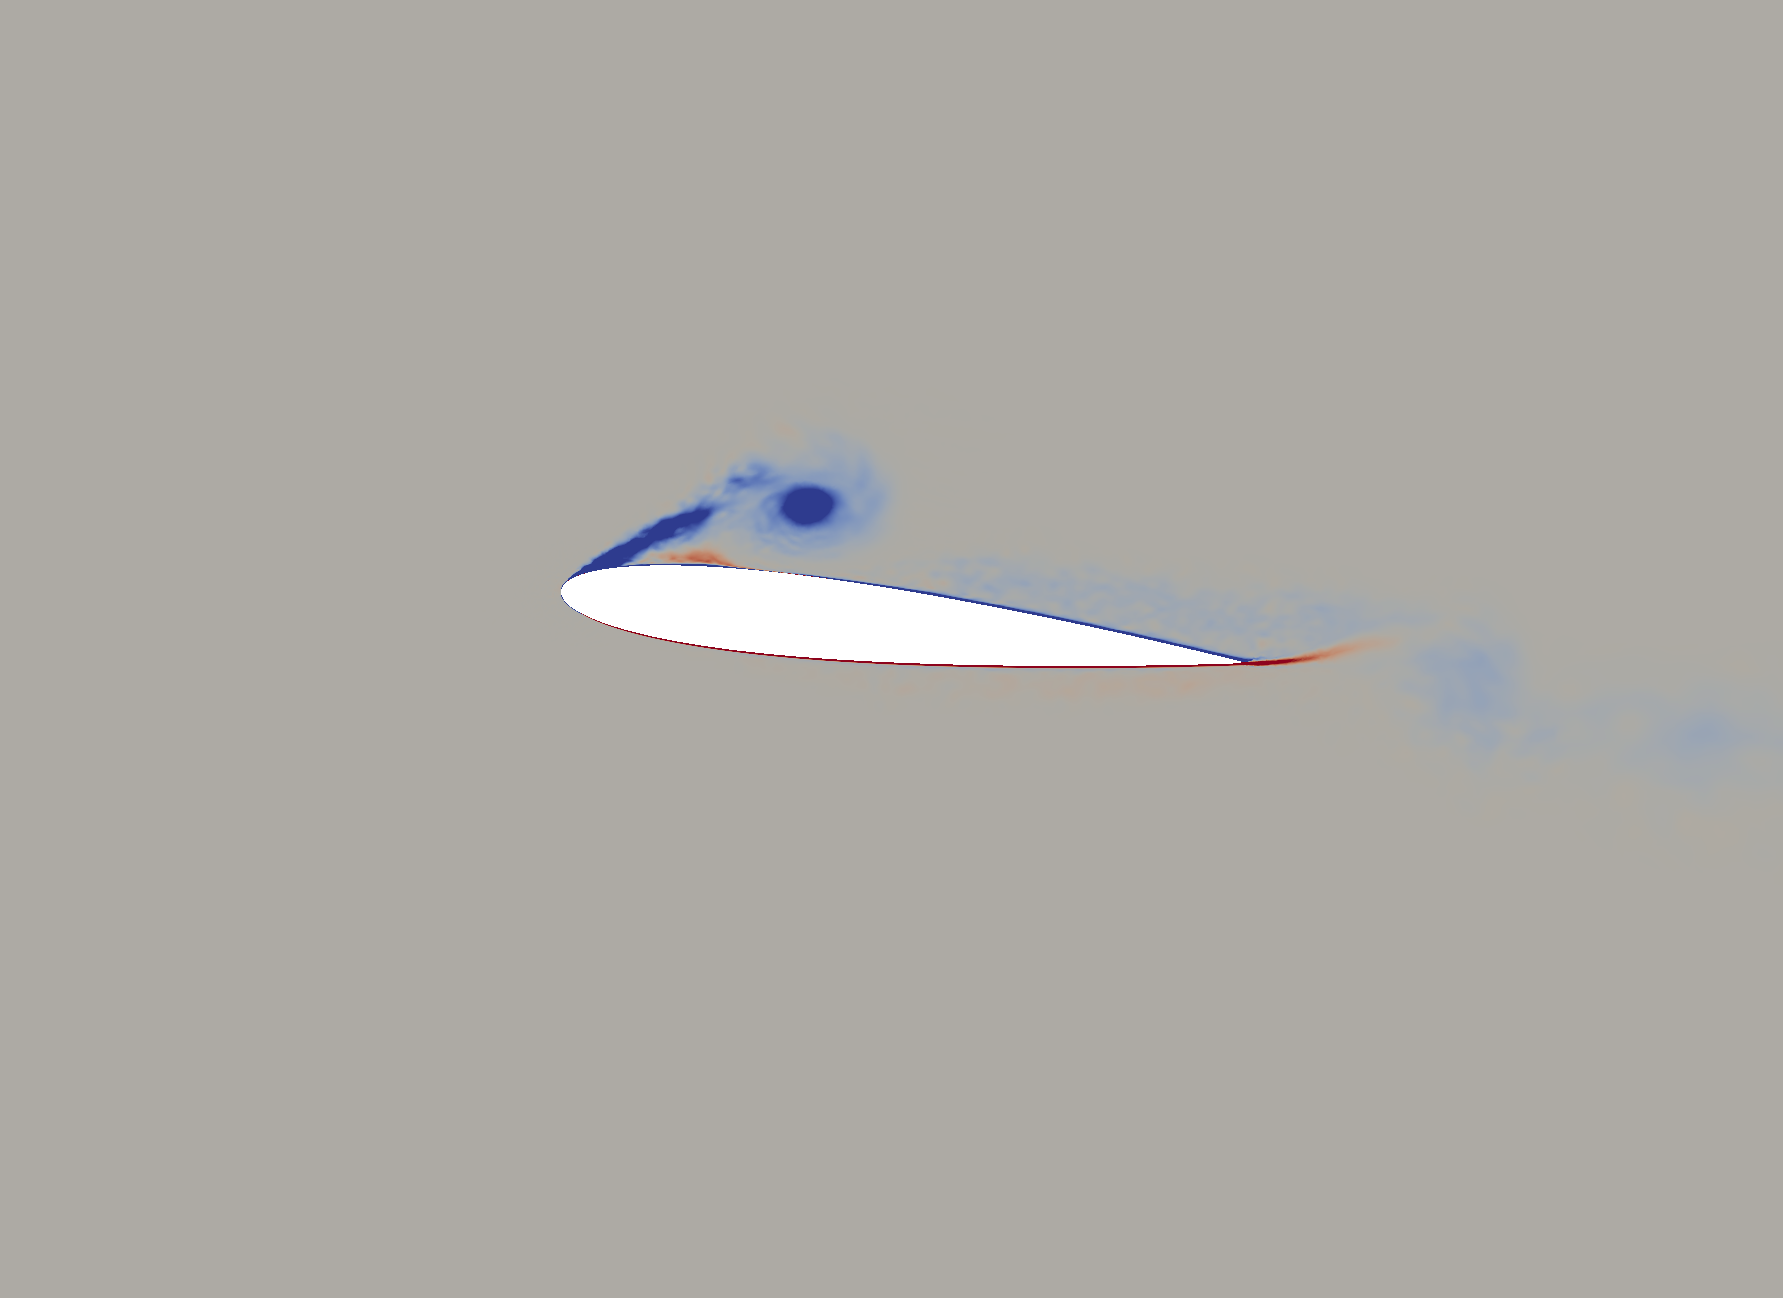
\includegraphics[width=1\textwidth]{figures/Vorticity_plots/Re_1m_1pt0/phase_315.png}
		\caption{$Re=1e6$, $\psi$ = $315^\circ$, $\tilde{t}=0.875$}
		\label{fig:Re_1m_1pt0_phi315}
	\end{subfigure}
	
	\begin{subfigure}[b]{0.32\textwidth}
		\centering
		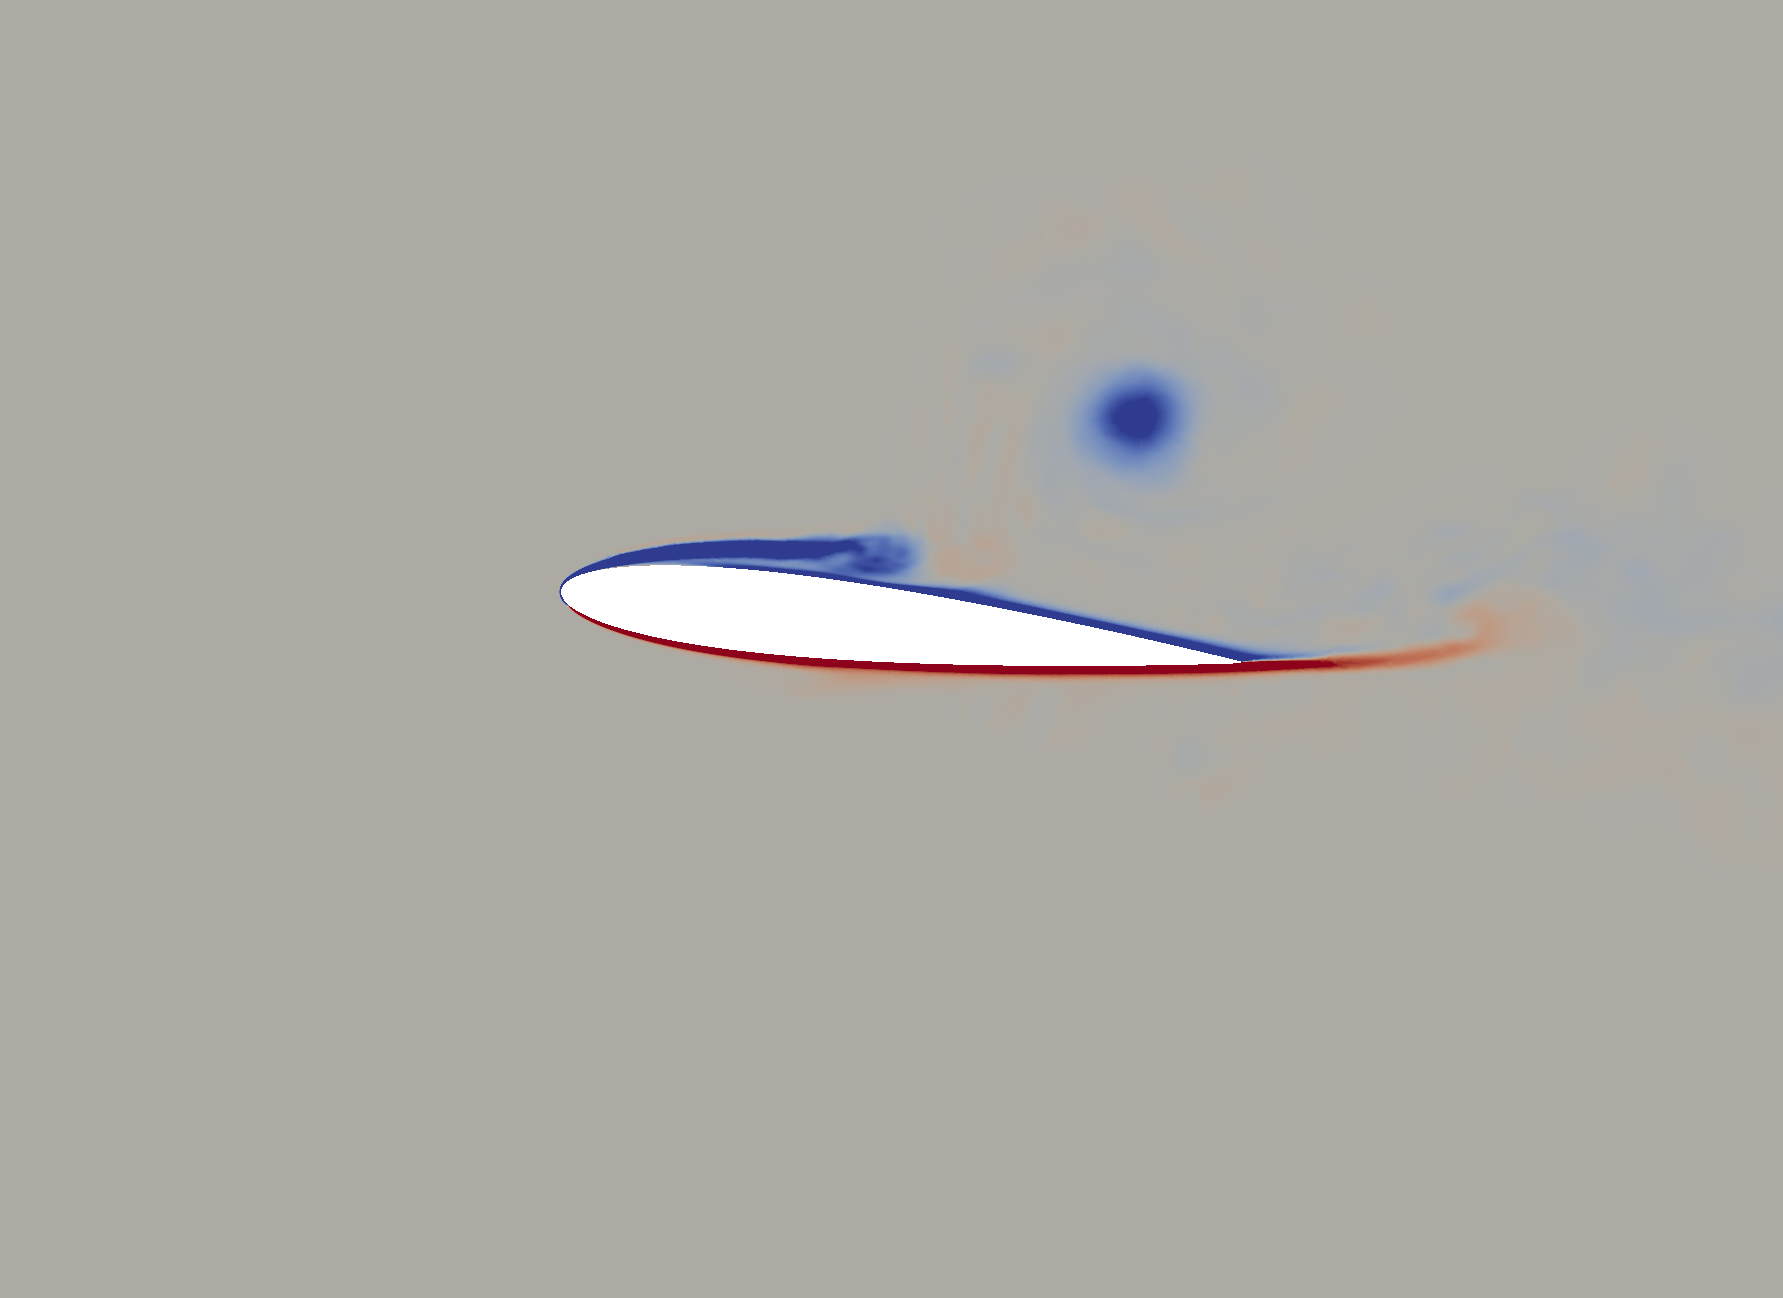
\includegraphics[width=1\textwidth]{figures/Vorticity_plots/Re_40k_1pt0/phase_330.png}
		\caption{$Re=4e4$, $\psi$ = $330^\circ$, $\tilde{t}=0.917$}
		\label{fig:Re_40k_1pt0_phi330}
	\end{subfigure}
	\begin{subfigure}[b]{0.32\textwidth}
		\centering
		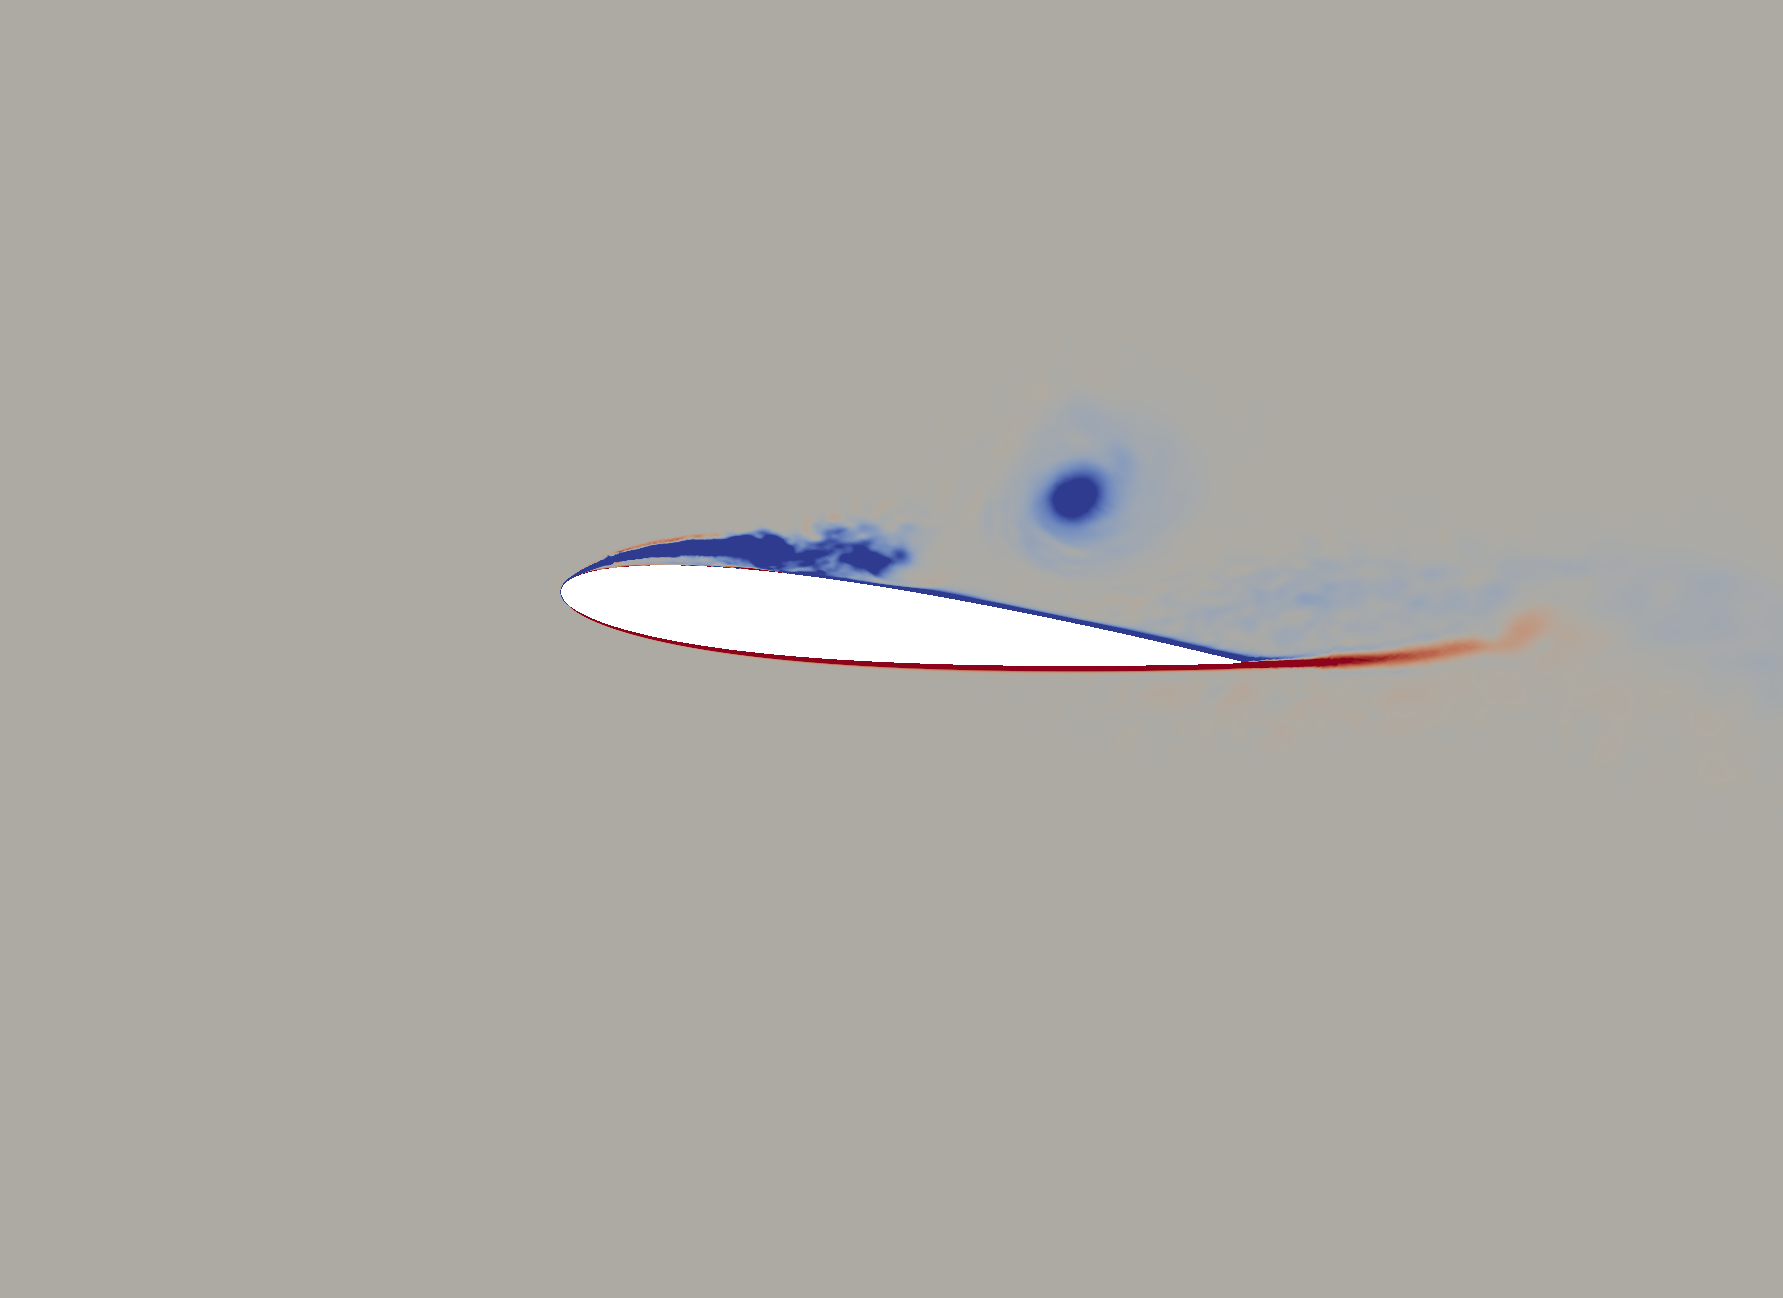
\includegraphics[width=1\textwidth]{figures/Vorticity_plots/Re_200k_1pt0/phase_330.png}
		\caption{$Re=2e5$, $\psi$ = $330^\circ$, $\tilde{t}=0.917$}
		\label{fig:Re_200k_1pt0_phi330}
	\end{subfigure}
	\begin{subfigure}[b]{0.32\textwidth}
		\centering
		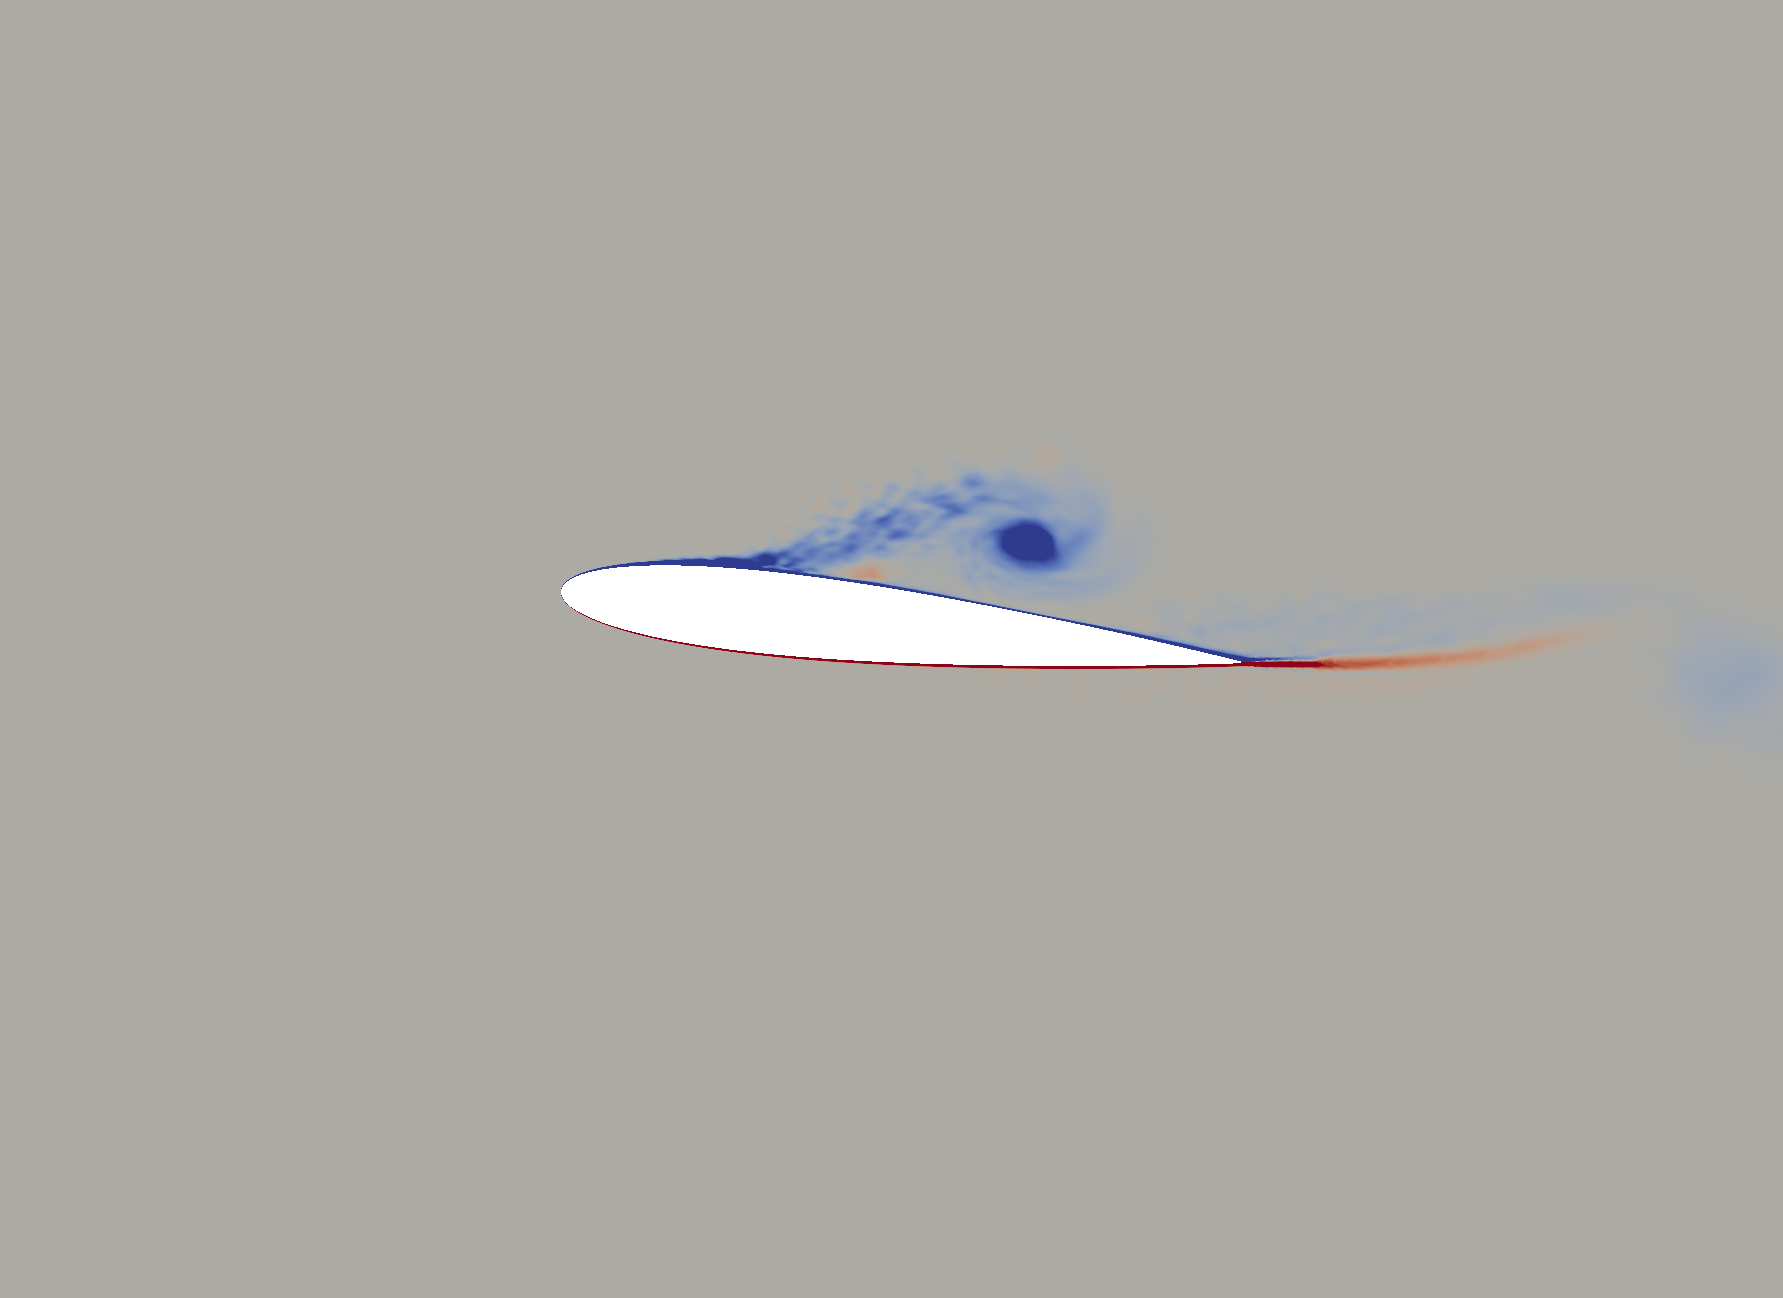
\includegraphics[width=1\textwidth]{figures/Vorticity_plots/Re_1m_1pt0/phase_330.png}
		\caption{$Re=1e6$,$\psi$ = $330^\circ$, $\tilde{t}=0.917$}
		\label{fig:Re_1m_1pt0_phi330}
	\end{subfigure}
	
	\begin{subfigure}[b]{0.32\textwidth}
		\centering
		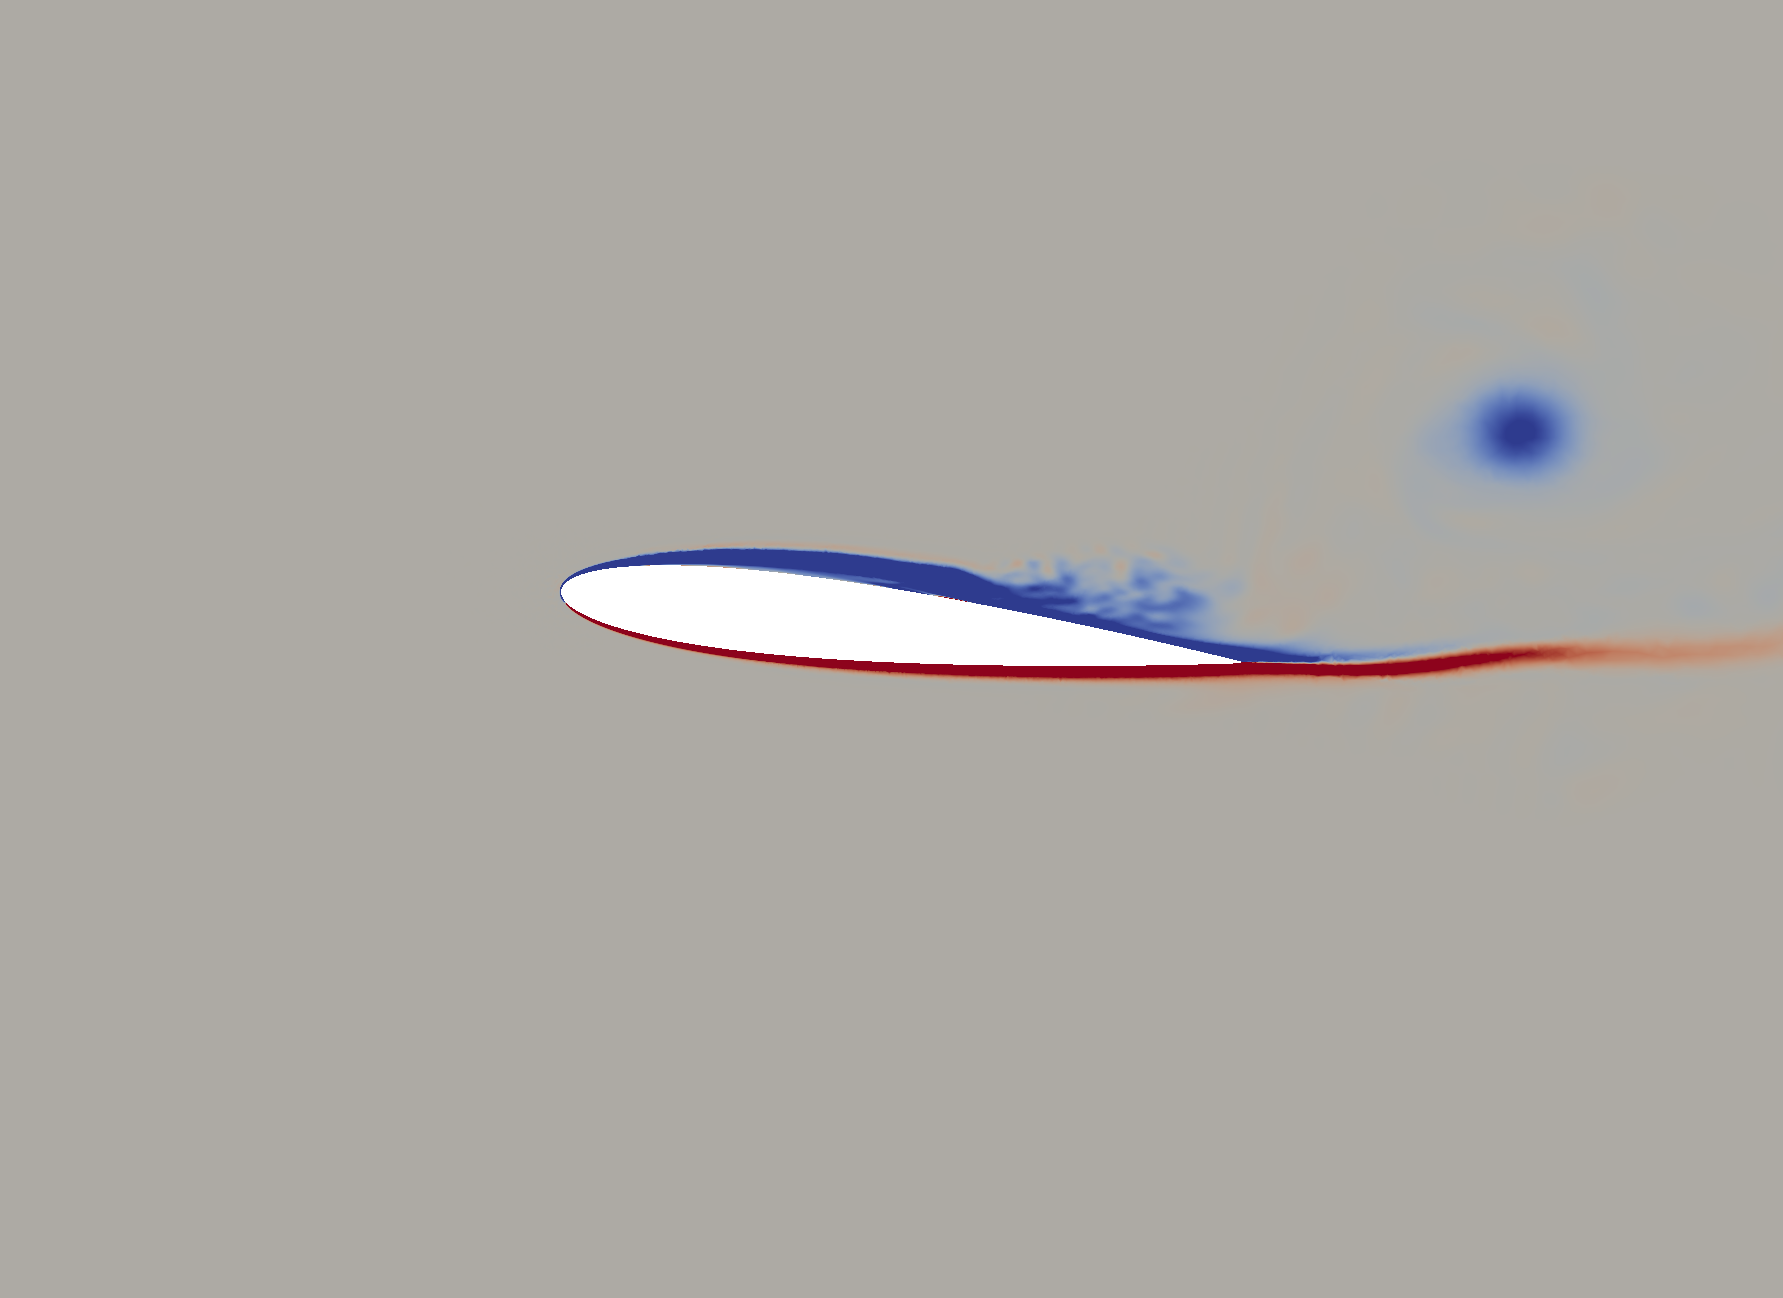
\includegraphics[width=1\textwidth]{figures/Vorticity_plots/Re_40k_1pt0/phase_345.png}
		\caption{$Re=4e4$, $\psi$ = $345^\circ$, $\tilde{t}=0.958$}
		\label{fig:Re_40k_1pt0_phi345}
	\end{subfigure}
	\begin{subfigure}[b]{0.32\textwidth}
		\centering
		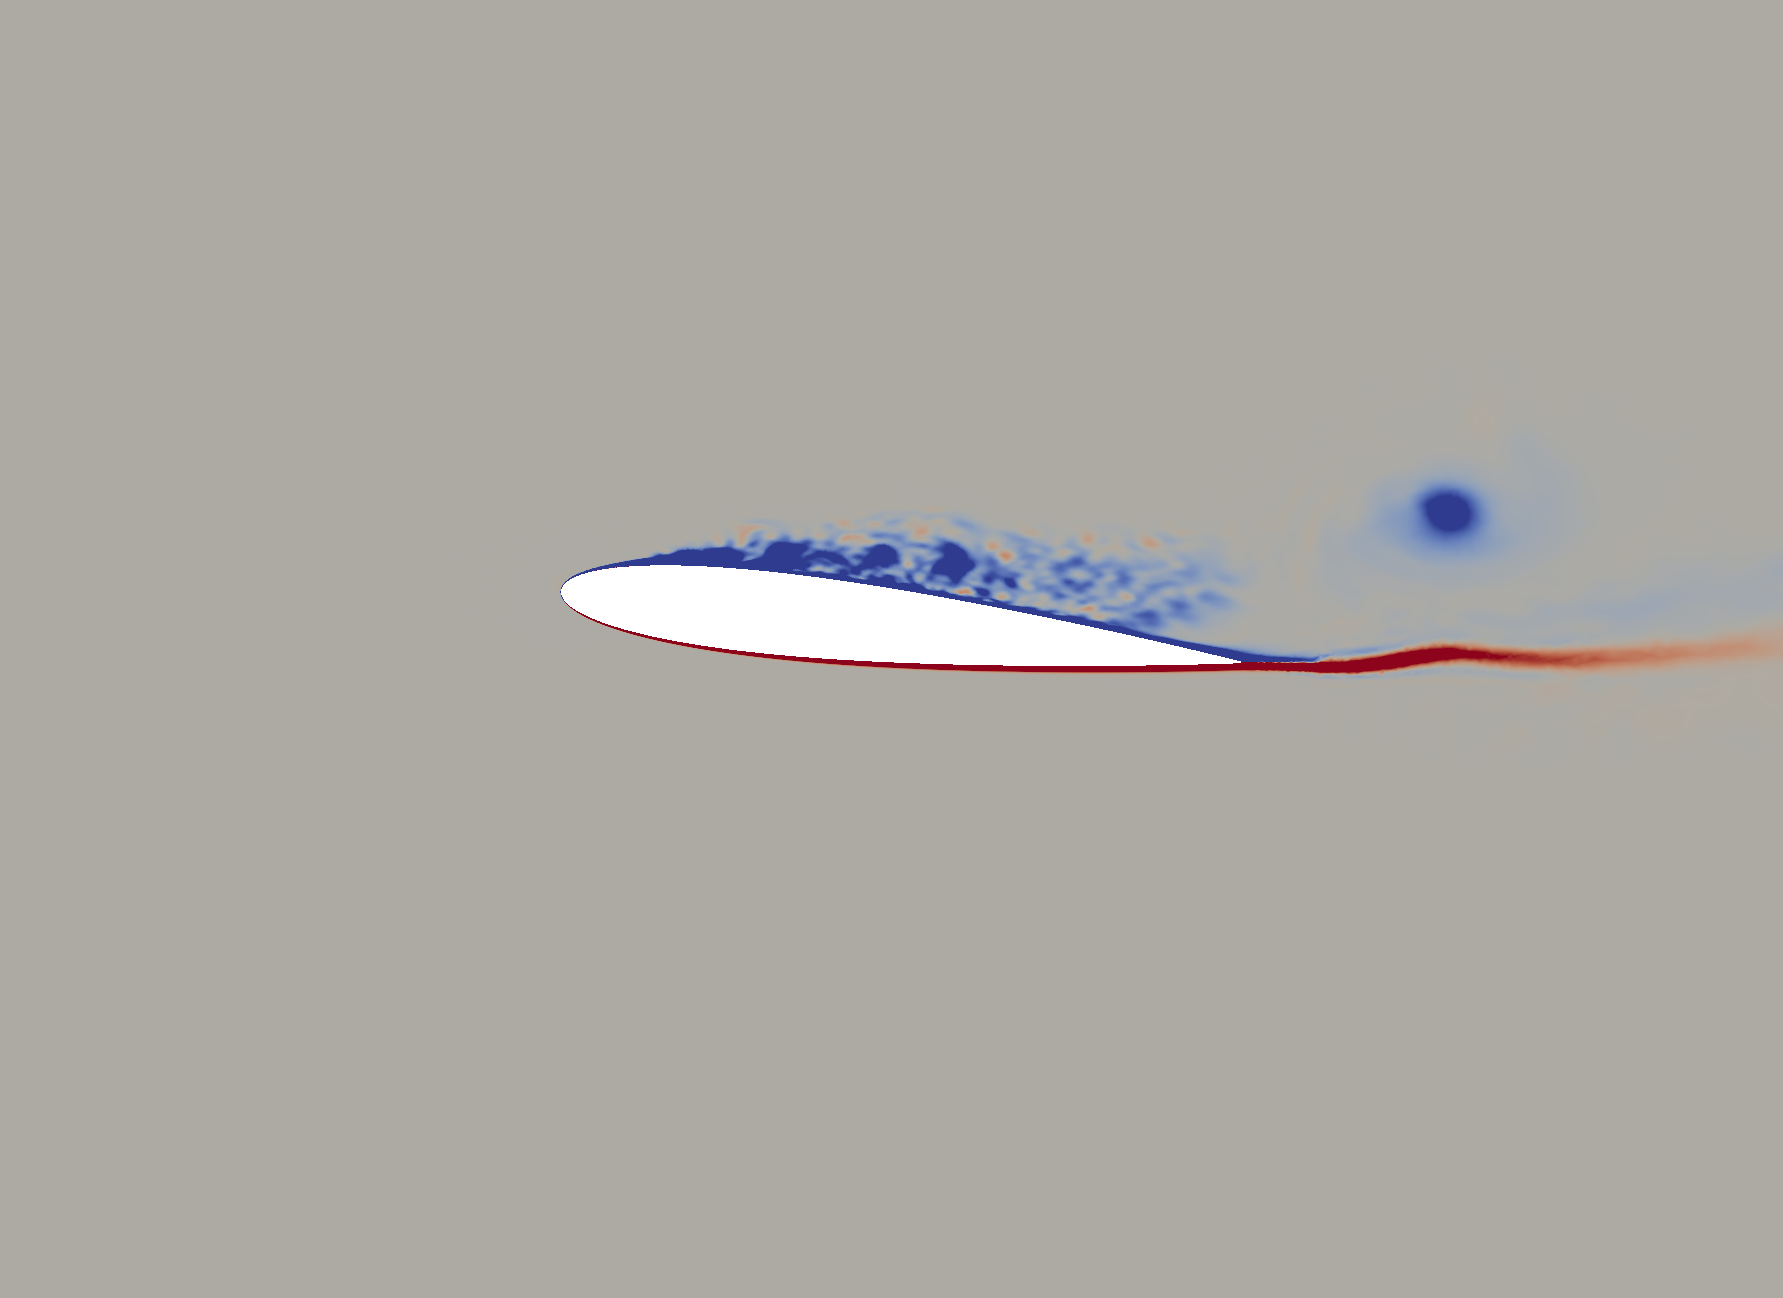
\includegraphics[width=1\textwidth]{figures/Vorticity_plots/Re_200k_1pt0/phase_345.png}
		\caption{$Re=2e5$, $\psi$ = $345^\circ$, $\tilde{t}=0.958$}
		\label{fig:Re_200k_1pt0_phi345}
	\end{subfigure}
	\begin{subfigure}[b]{0.32\textwidth}
		\centering
		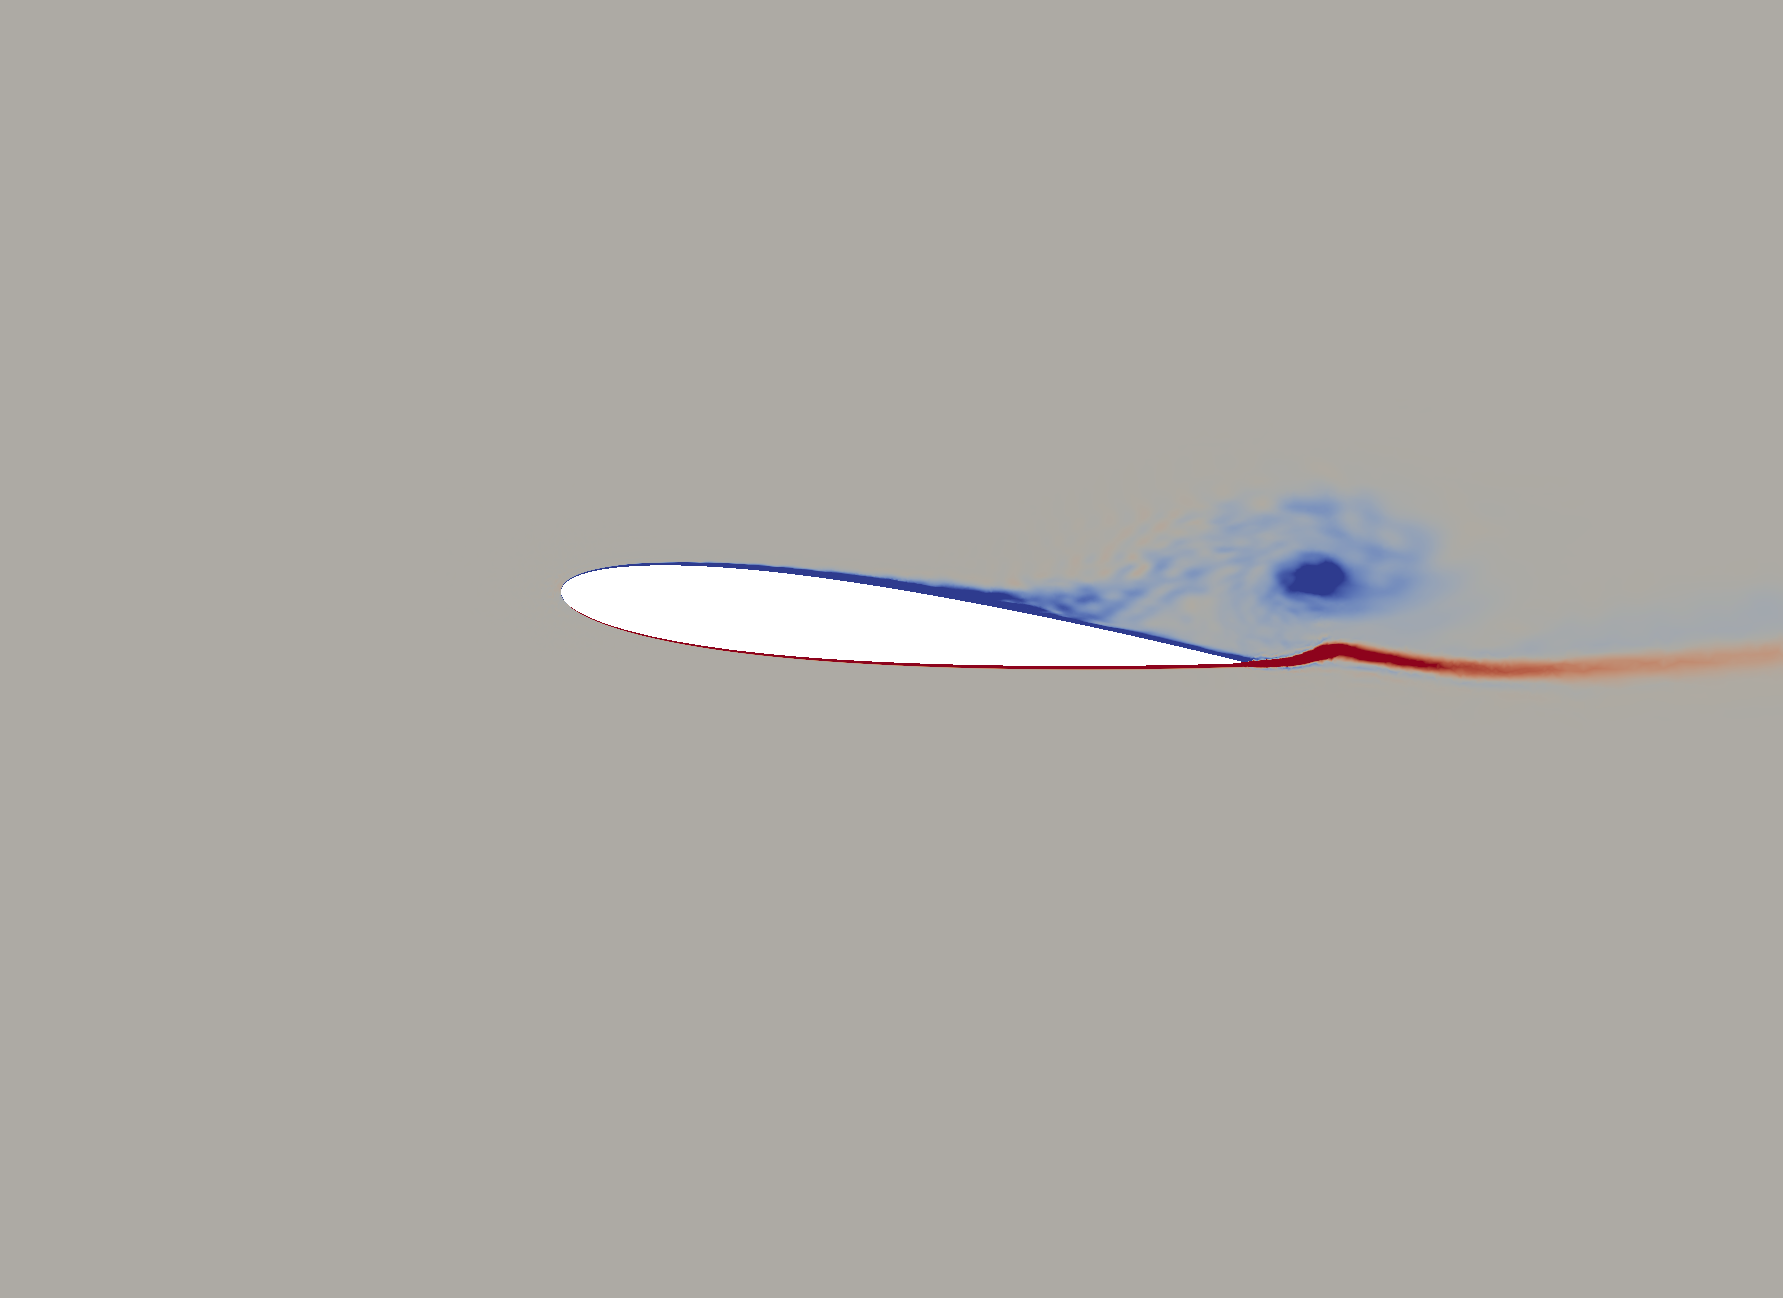
\includegraphics[width=1\textwidth]{figures/Vorticity_plots/Re_1m_1pt0/phase_345.png}
		\caption{$Re=1e6$, $\psi$ = $345^\circ$, $\tilde{t}=0.958$}
		\label{fig:Re_1m_1pt0_phi345}
	\end{subfigure}	
\caption{Spanwise vorticity at 8 different phases for $Re$=40,000 (left column), 200,000 (middle column) and 1,000,000 (right column) at $\mu_{sect}$ = 1.0}
\label{fig:vortScreen_1pt0}
\end{figure}


At $\psi$=$225^\circ$, the flow is separated near the leading edge for the lowest Reynolds number of $Re$=40,000 and the separated shear layer rolls up into an LEV, see Figure~\ref{fig:Re_200k_1pt0_phi225}.
For the other two higher Reynolds numbers, the flow remains attached.
Similarly, at $Re$=200,000 the separated shear layer rolls up into a smaller LEV at $\psi$=$240^\circ$, while for $Re$=1,000,000 this occurs at $\psi$=$270^\circ$ (see Figure \ref{fig:Re_1m_1pt0_phi270}).
As the Reynolds number increases the LEV is formed later in the cycle.
In summary, as the airfoil retreats vorticity accumulates around the airfoil and separated shear layer rolls up into a distinct vortex near the leading edge (i.e., an LEV) over the suction or upper side of the airfoil.

In subsequent phases, LEV is ejected into the outer flow and advects.
The flow on the suction or upper side reattaches as the leading edge vortex passes over the airfoil.
Flow also separates and reattaches on the pressure or lower side, e.g., see marginal flow separation at the trailing edge on the lower side in Fig \ref{fig:Re_40k_1pt0_phi225}.

It is important to note the differences in LEV evolution with different Reynolds number even though the overall trend of the LEV evolution is similar between different Reynolds number.
As already noted, the phase at which the LEV is formed changes with Reynolds number.
Further, the size and vertical position of the LEV also changes significantly with Reynolds number.
This aspect is discussed in Section \ref{sec:LEV}.

Figure \ref{fig:vortScreen_1pt2} shows the spanwise vorticity for the higher advance ratio of $\mu_{sect}$=1.2.
Again, 8 different phases over the retreating phase of the cycle are shown and the range is selected to be [-10,10]$\times U_\infty /C$.
As in the $\mu_{sect}=1.0$ case, at $\psi$=$195^\circ$ the flow over the airfoil is mostly attached in the $\mu_{sect}=1.2$ case.
As before, the boundary layer is much thicker for the lowest Reynolds number of $Re$=40,000 as compared to the other two higher Reynolds numbers.

At $\psi$=$225^\circ$, the flow is fully separated for the lowest Reynolds number of $Re$=40,000 and the separated shear layer is rolled up into an LEV, see Figure~\ref{fig:Re_40k_1pt2_phi225}.
Similarly, at $Re$=200,000 a smaller LEV is seen at $\psi$=$225^\circ$ (see Figure \ref{fig:Re_200k_1pt2_phi225}), while for $Re$=1,000,000, LEV is observed at $\psi$=$240^\circ$.
As before, as the Reynolds number increases the LEV is formed later in the cycle.
On the other hand, as the advance ratio increases it is formed earlier in the cycle (for a given Reynolds number).
For example, for $Re$=1,000,000, the LEV is formed at an earlier phase for $\mu_{sect}=1.2$ as compared to $\mu_{sect}=1.0$.
Again, as the airfoil retreats vorticity accumulates and shear layer rolls up into a distinct LEV over the suction or upper side of the airfoil.

In subsequent phases, LEV is ejected into the outer flow and advects while the flow reattaches.
However, at the higher advance ratio of $\mu_{sect}$=1.2 the LEV initially moves to the left past the (geometric) leading edge of the airfoil.
This is because at $\mu_{sect}$=1.2, the relative flow velocity becomes negative and a reversed flow condition is reached.
Again, it is important to note the differences in LEV evolution with different Reynolds number for the advance ratio of $\mu_{sect}=1.2$.
As already noted, the size, position and phase of formation of LEV changes significantly with Reynolds number.
This aspect is discussed further in Section \ref{sec:LEV}.

\begin{figure}[H]
	\centering
	
	\begin{subfigure}[b]{0.32\textwidth}
		\centering
		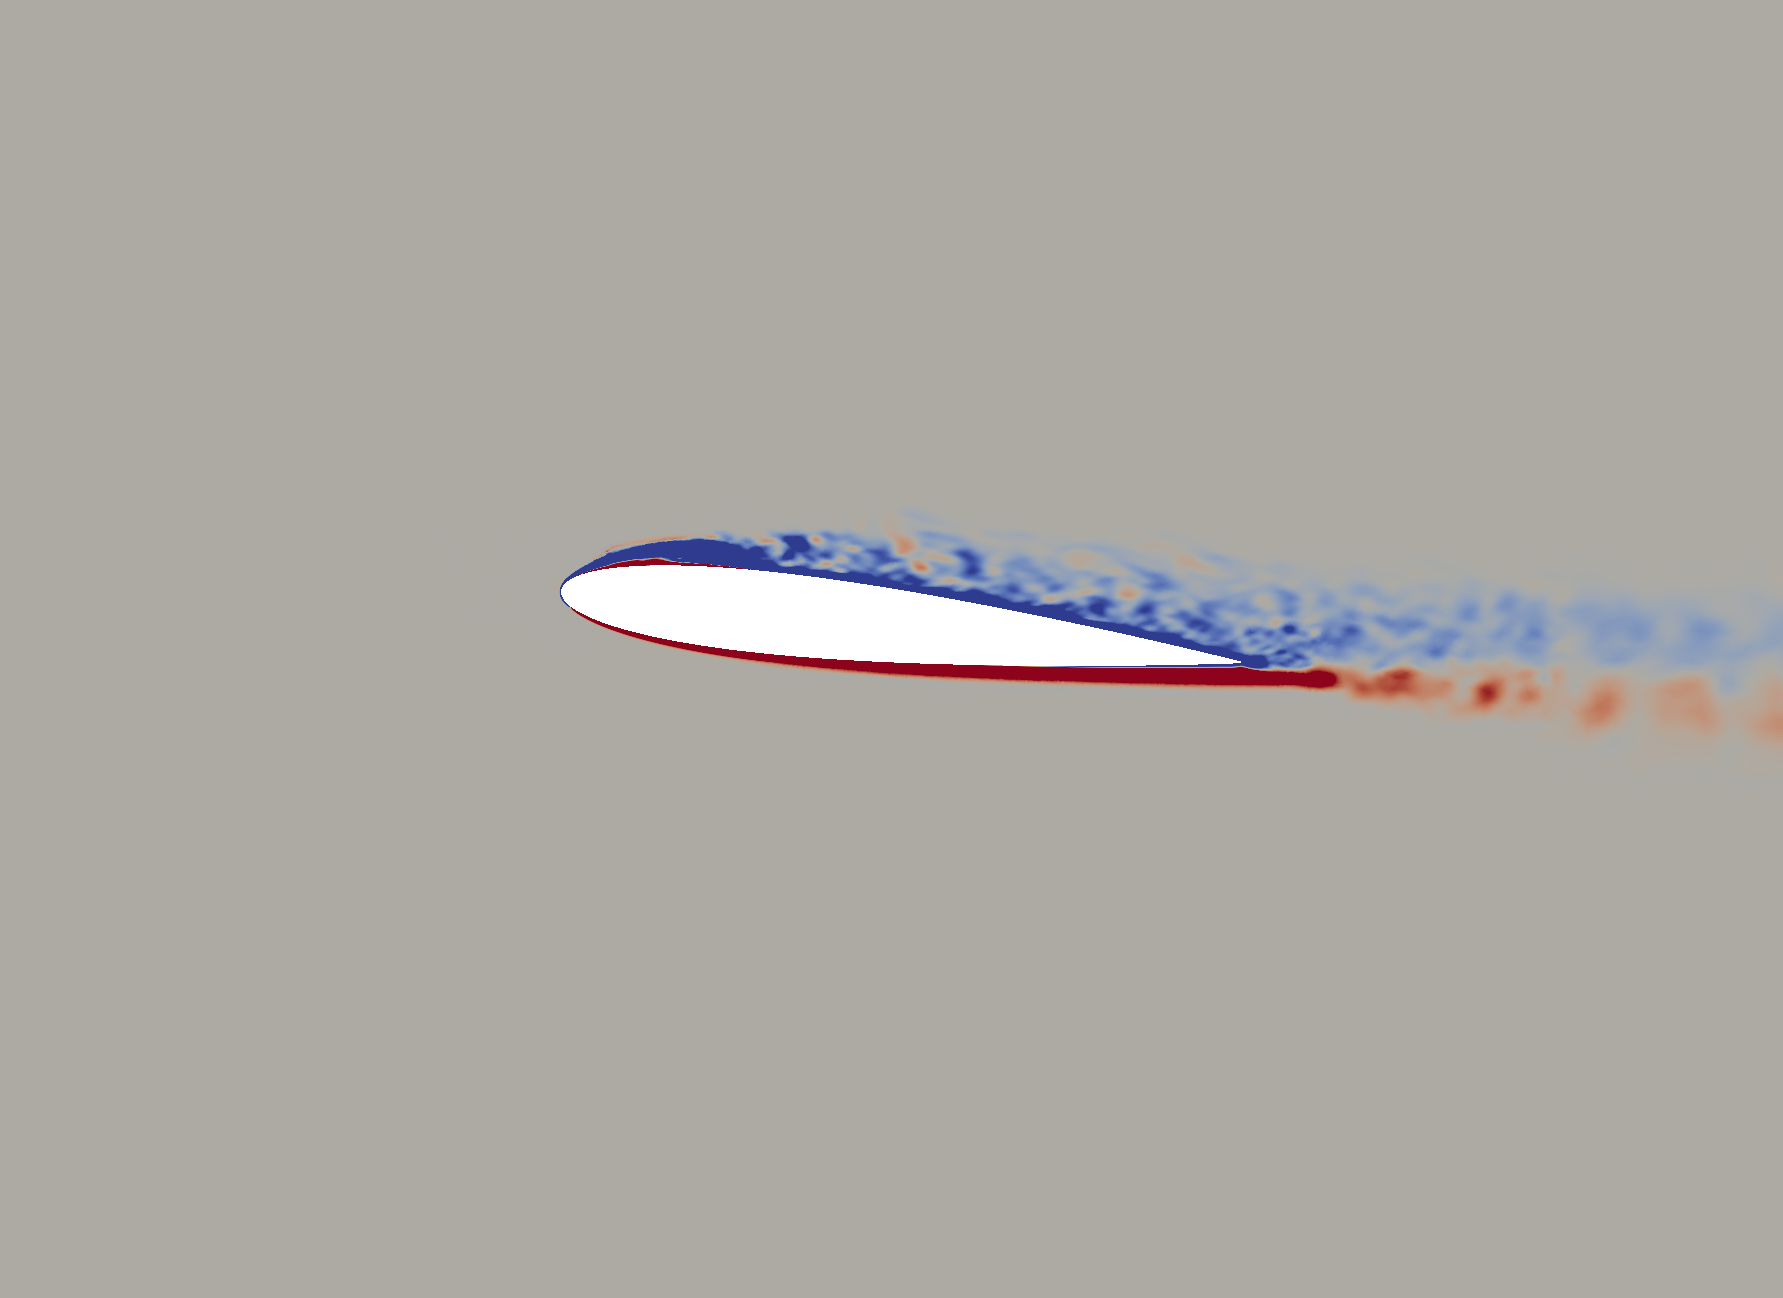
\includegraphics[width=1\textwidth]{figures/Vorticity_plots/Re_40k_1pt2/phase_195.png}
		\caption{$Re= 4e4$, $\psi$ = $195^\circ$, $\tilde{t}=0.542$}
		\label{fig:Re_40k_1pt2_phi195}
	\end{subfigure}
	\begin{subfigure}[b]{0.32\textwidth}
		\centering
		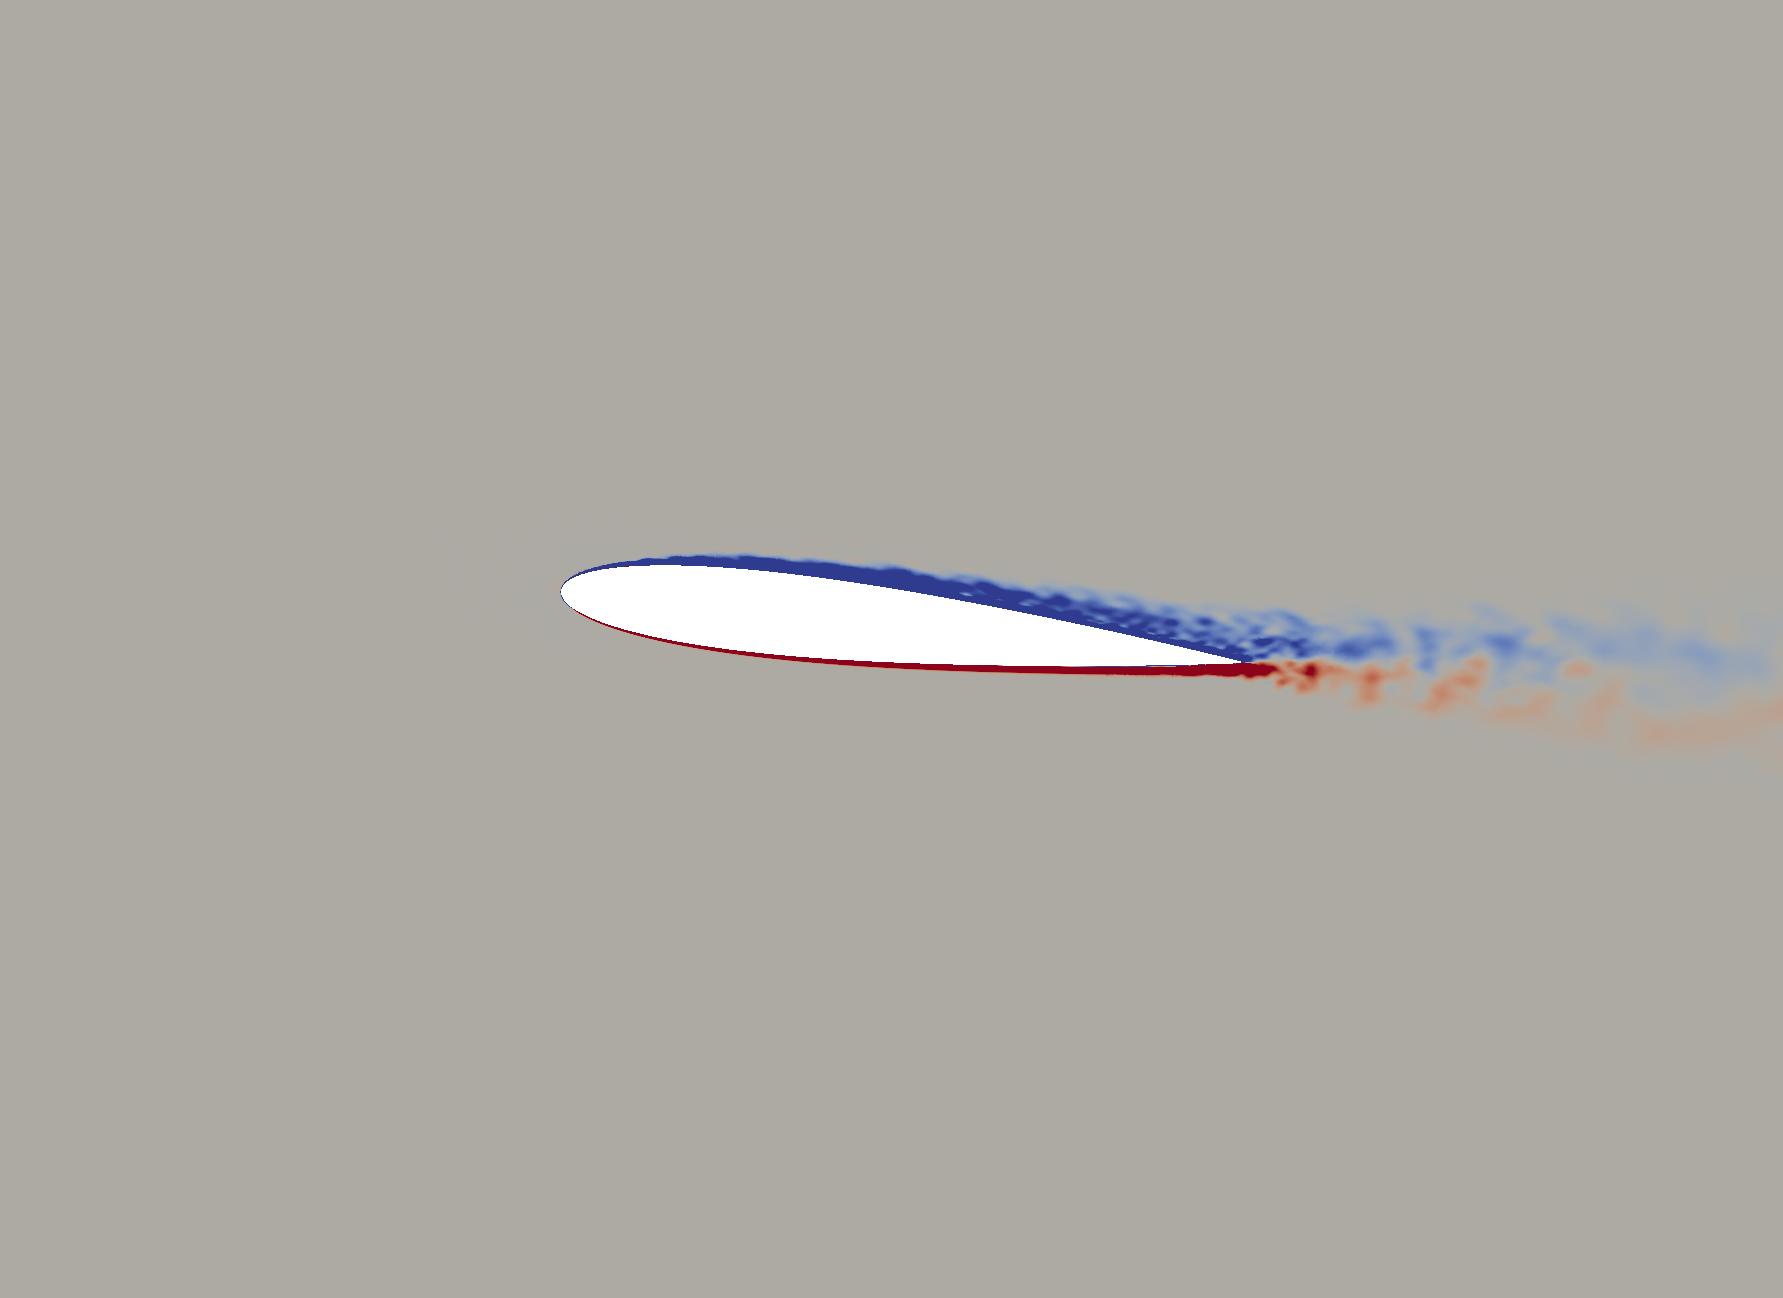
\includegraphics[width=1\textwidth]{figures/Vorticity_plots/Re_200k_1pt2/phase_195.png}
		\caption{$Re=2e5$, $\psi$ = $195^\circ$, $\tilde{t}=0.542$}
		\label{fig:Re_200k_1pt2_phi195}
	\end{subfigure}
	\begin{subfigure}[b]{0.32\textwidth}
		\centering
		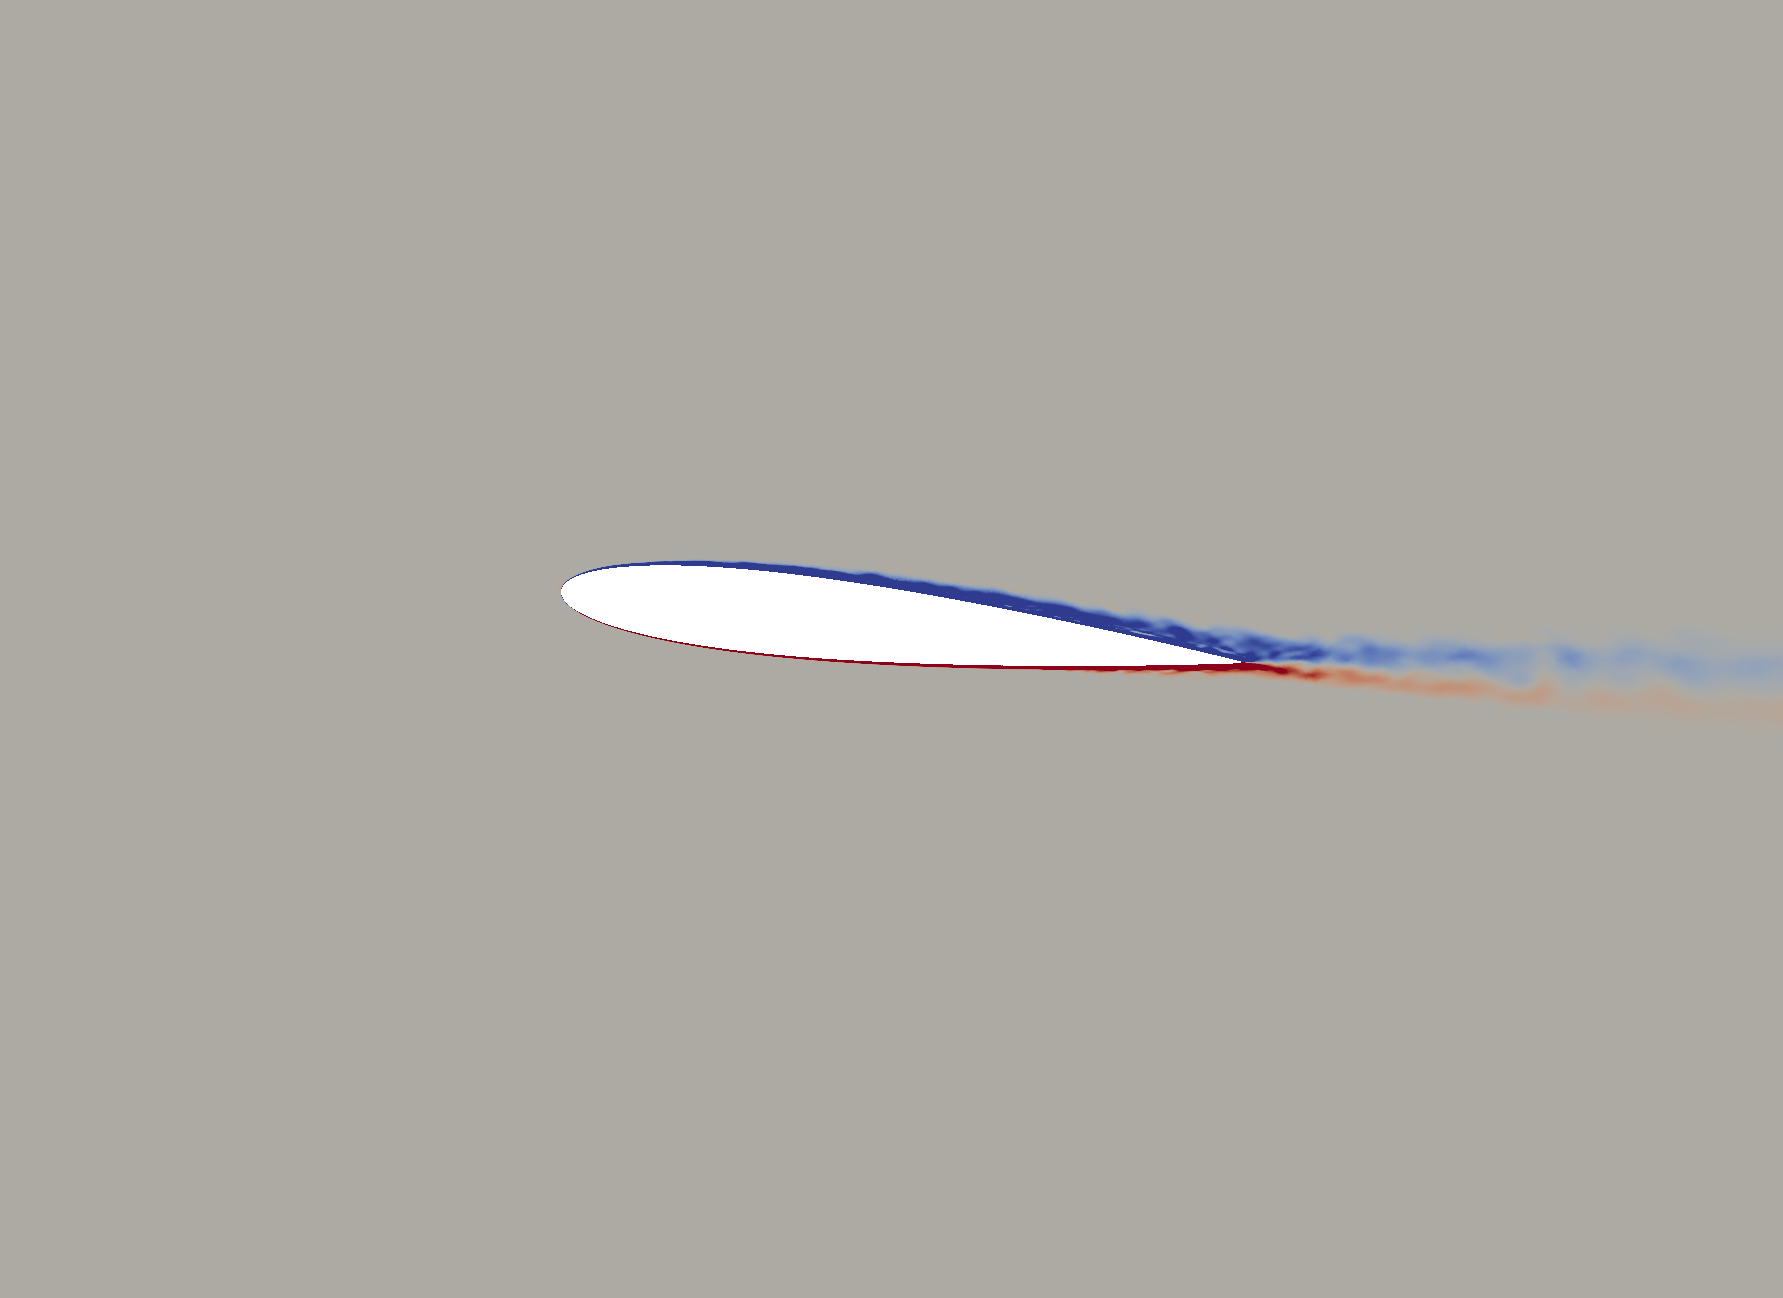
\includegraphics[width=1\textwidth]{figures/Vorticity_plots/Re_1m_1pt2/phase_195.png}
		\caption{$Re= 1e6$, $\psi$ = $195^\circ$, $\tilde{t}=0.542$}
		\label{fig:Re_1m_1pt2_phi195}
	\end{subfigure}
	
	\begin{subfigure}[b]{0.32\textwidth}
		\centering
		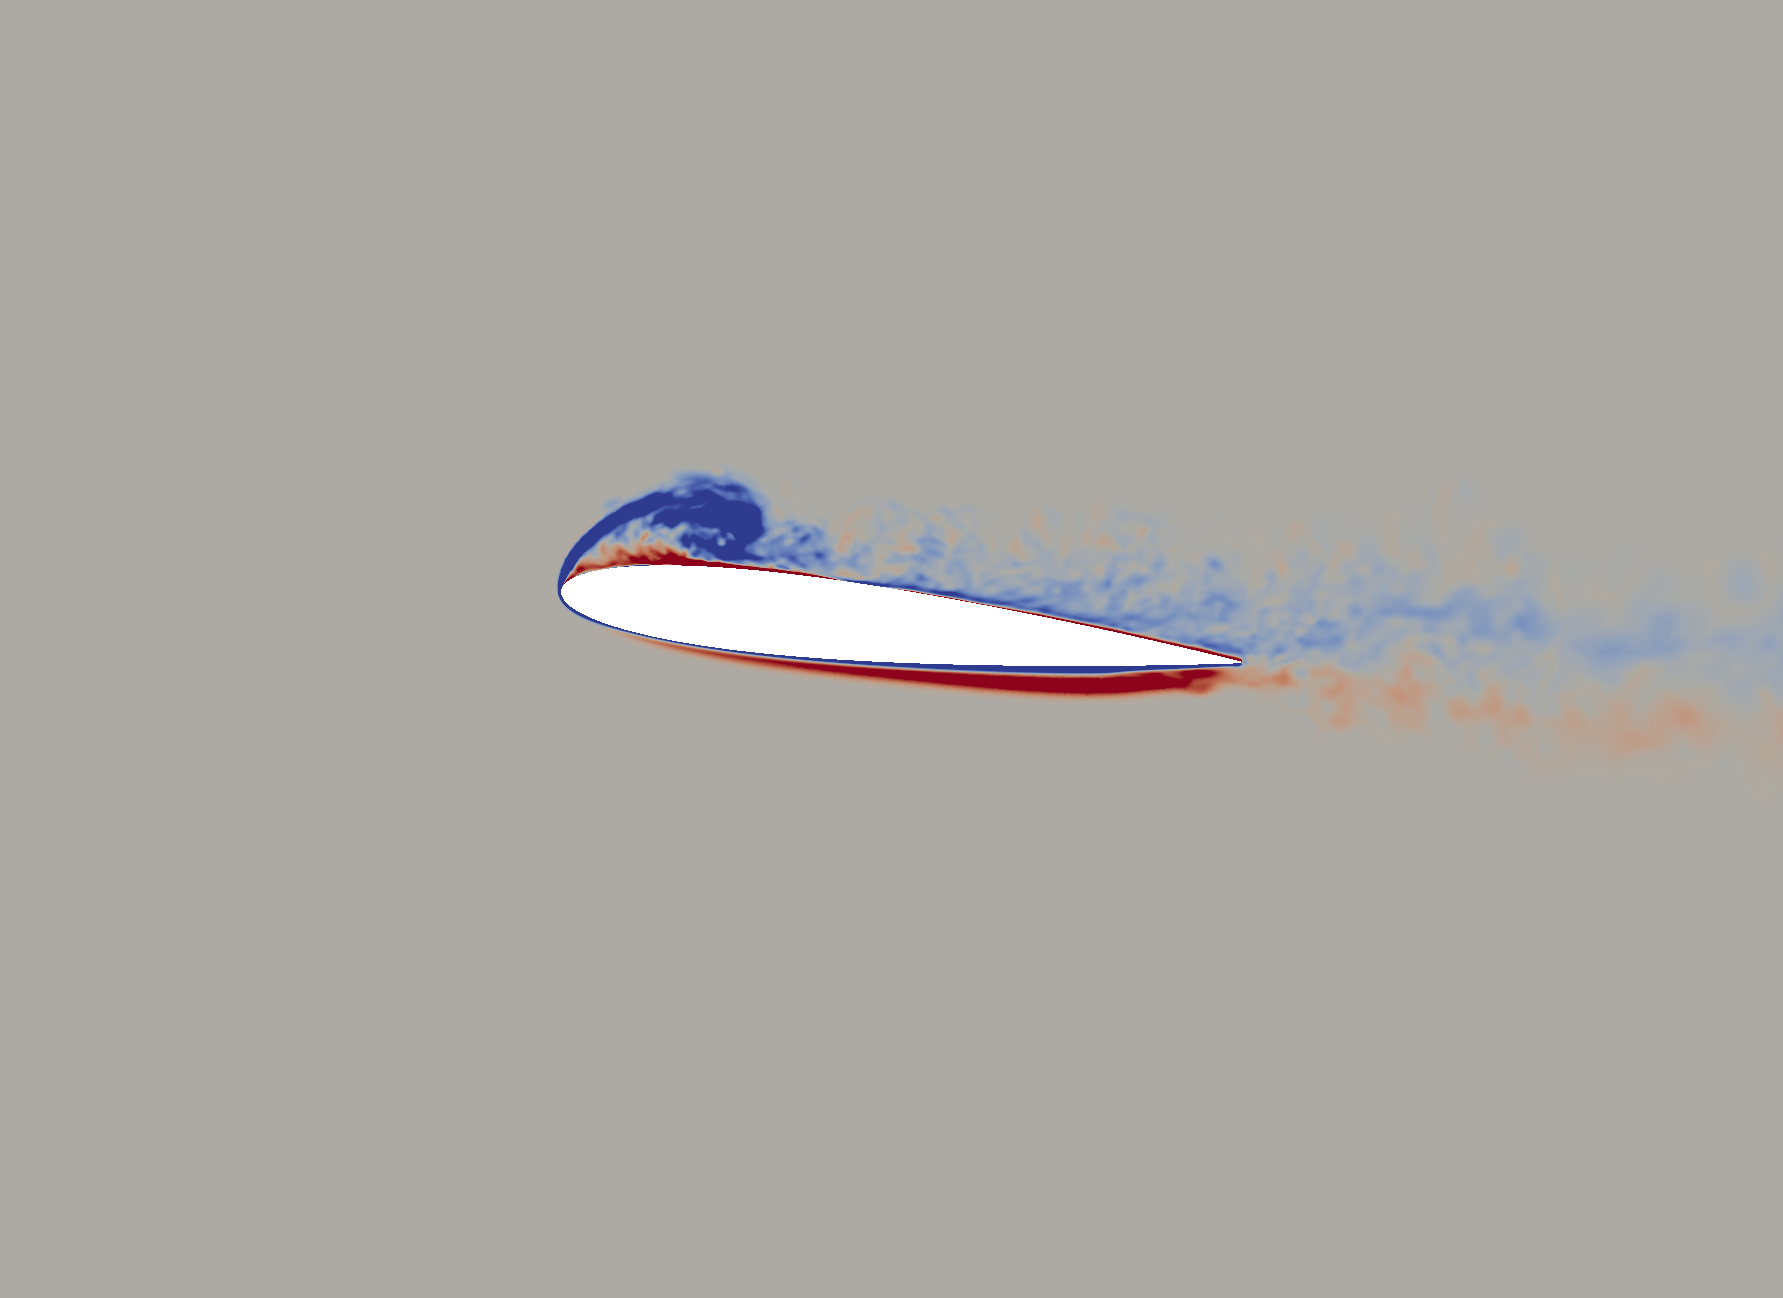
\includegraphics[width=1\textwidth]{figures/Vorticity_plots/Re_40k_1pt2/phase_225.png}
		\caption{$Re=4e4$, $\psi$ = $225^\circ$, $\tilde{t}=0.625$}
		\label{fig:Re_40k_1pt2_phi225}
	\end{subfigure}
	\begin{subfigure}[b]{0.32\textwidth}
		\centering
		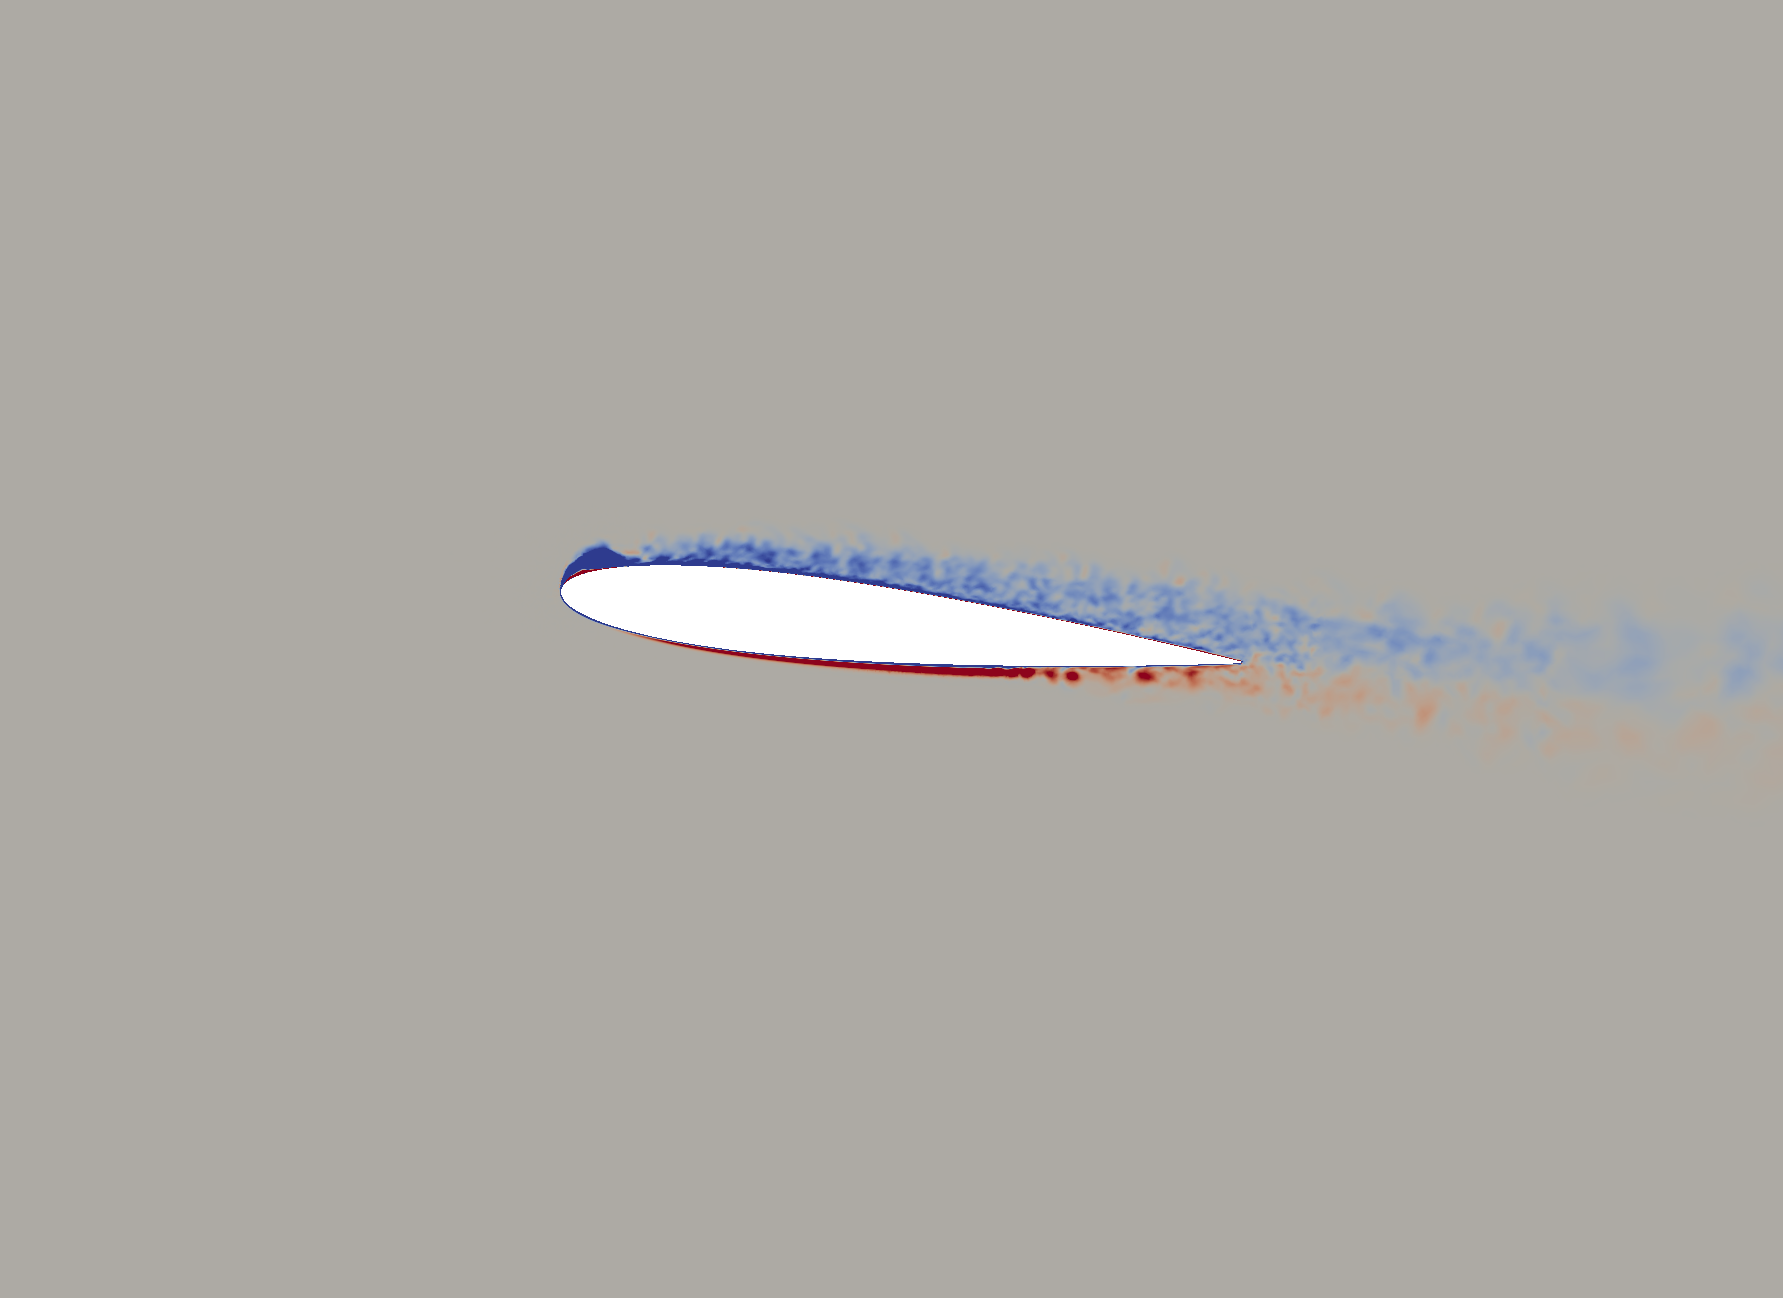
\includegraphics[width=1\textwidth]{figures/Vorticity_plots/Re_200k_1pt2/phase_225.png}
		\caption{$Re=2e5$, $\psi$ = $225^\circ$, $\tilde{t}=0.625$}
		\label{fig:Re_200k_1pt2_phi225}
	\end{subfigure}
	\begin{subfigure}[b]{0.32\textwidth}
		\centering
		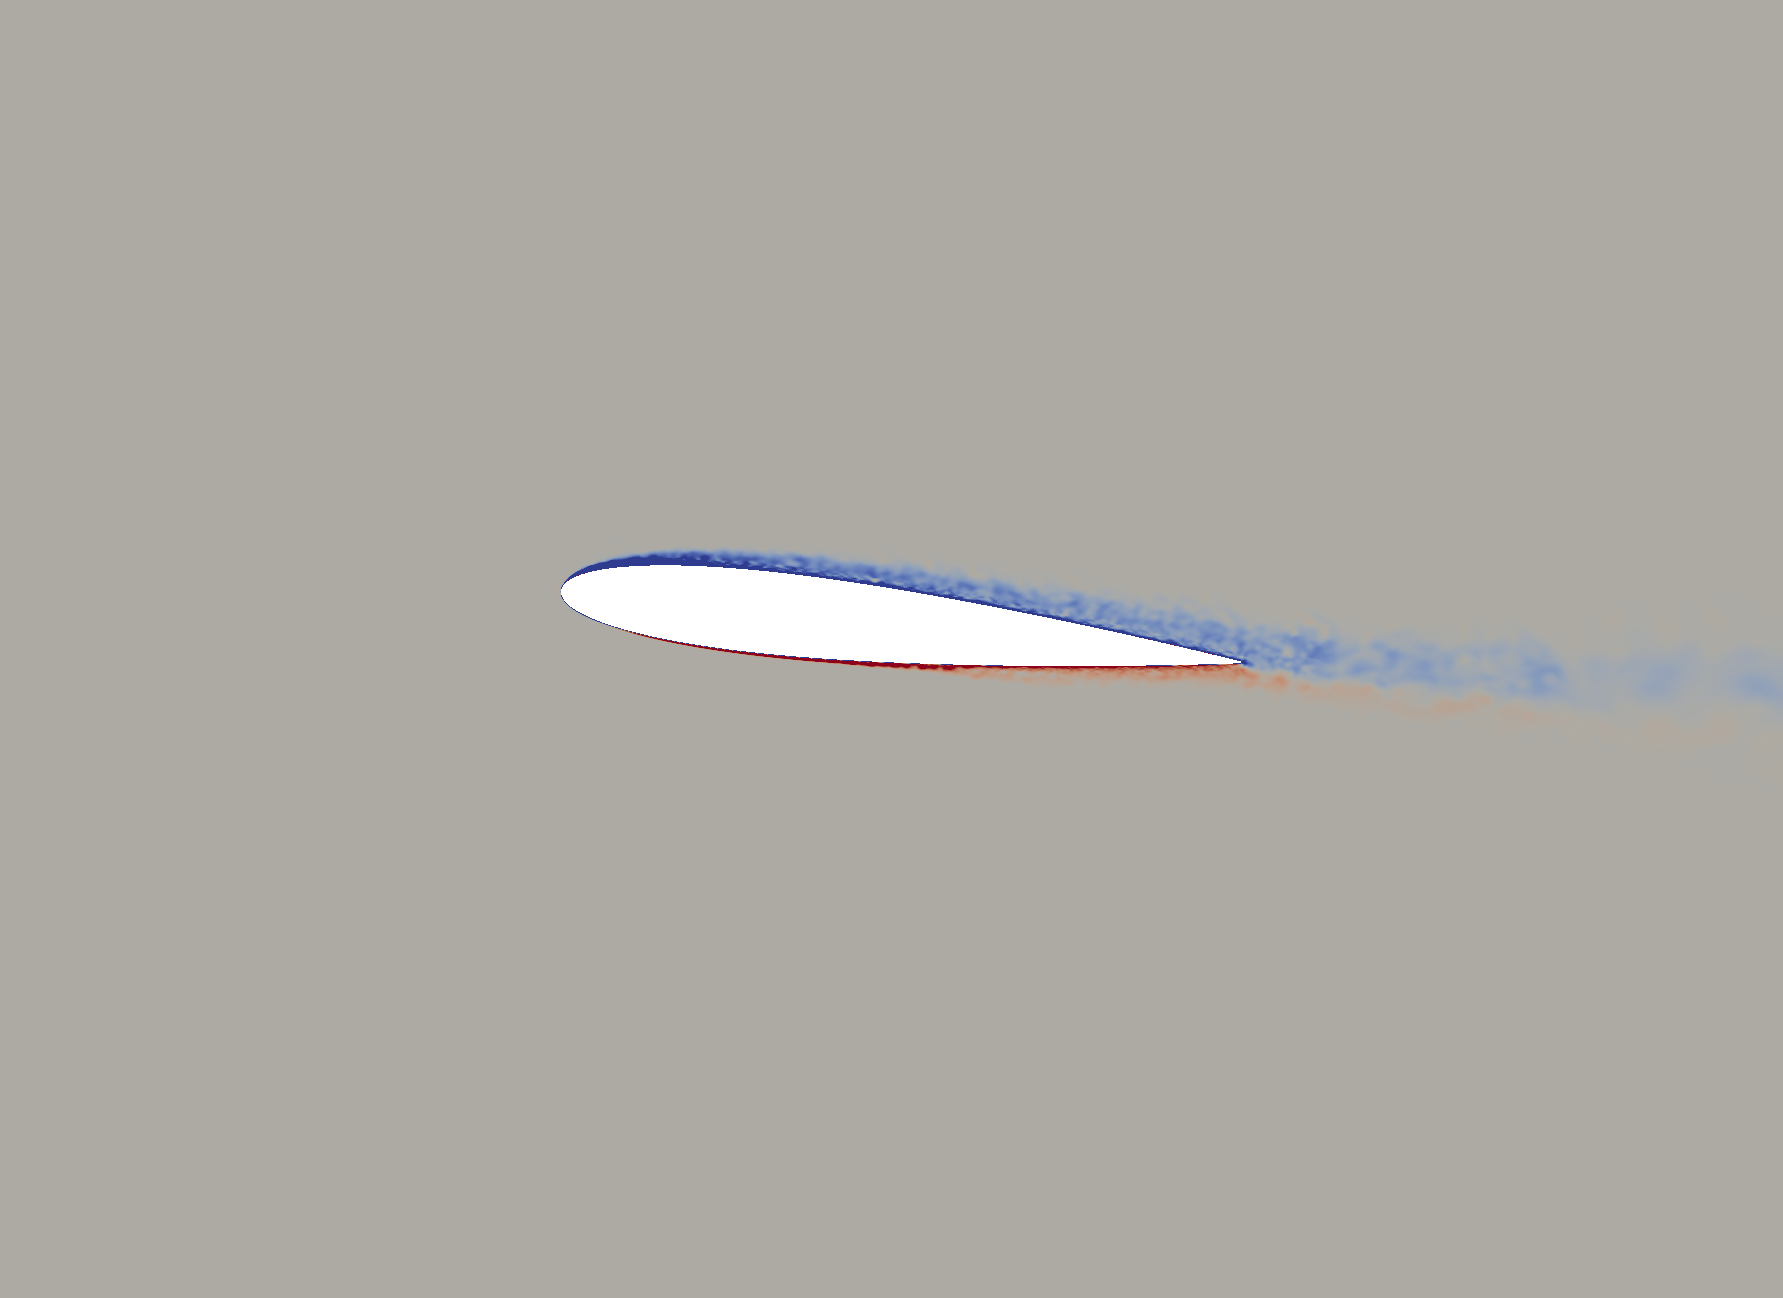
\includegraphics[width=1\textwidth]{figures/Vorticity_plots/Re_1m_1pt2/phase_225.png}
		\caption{$Re=1e6$, $\psi$ = $225^\circ$, $\tilde{t}=0.625$}
		\label{fig:Re_1m_1pt2_phi225}
	\end{subfigure}
	
	\begin{subfigure}[b]{0.32\textwidth}
		\centering
		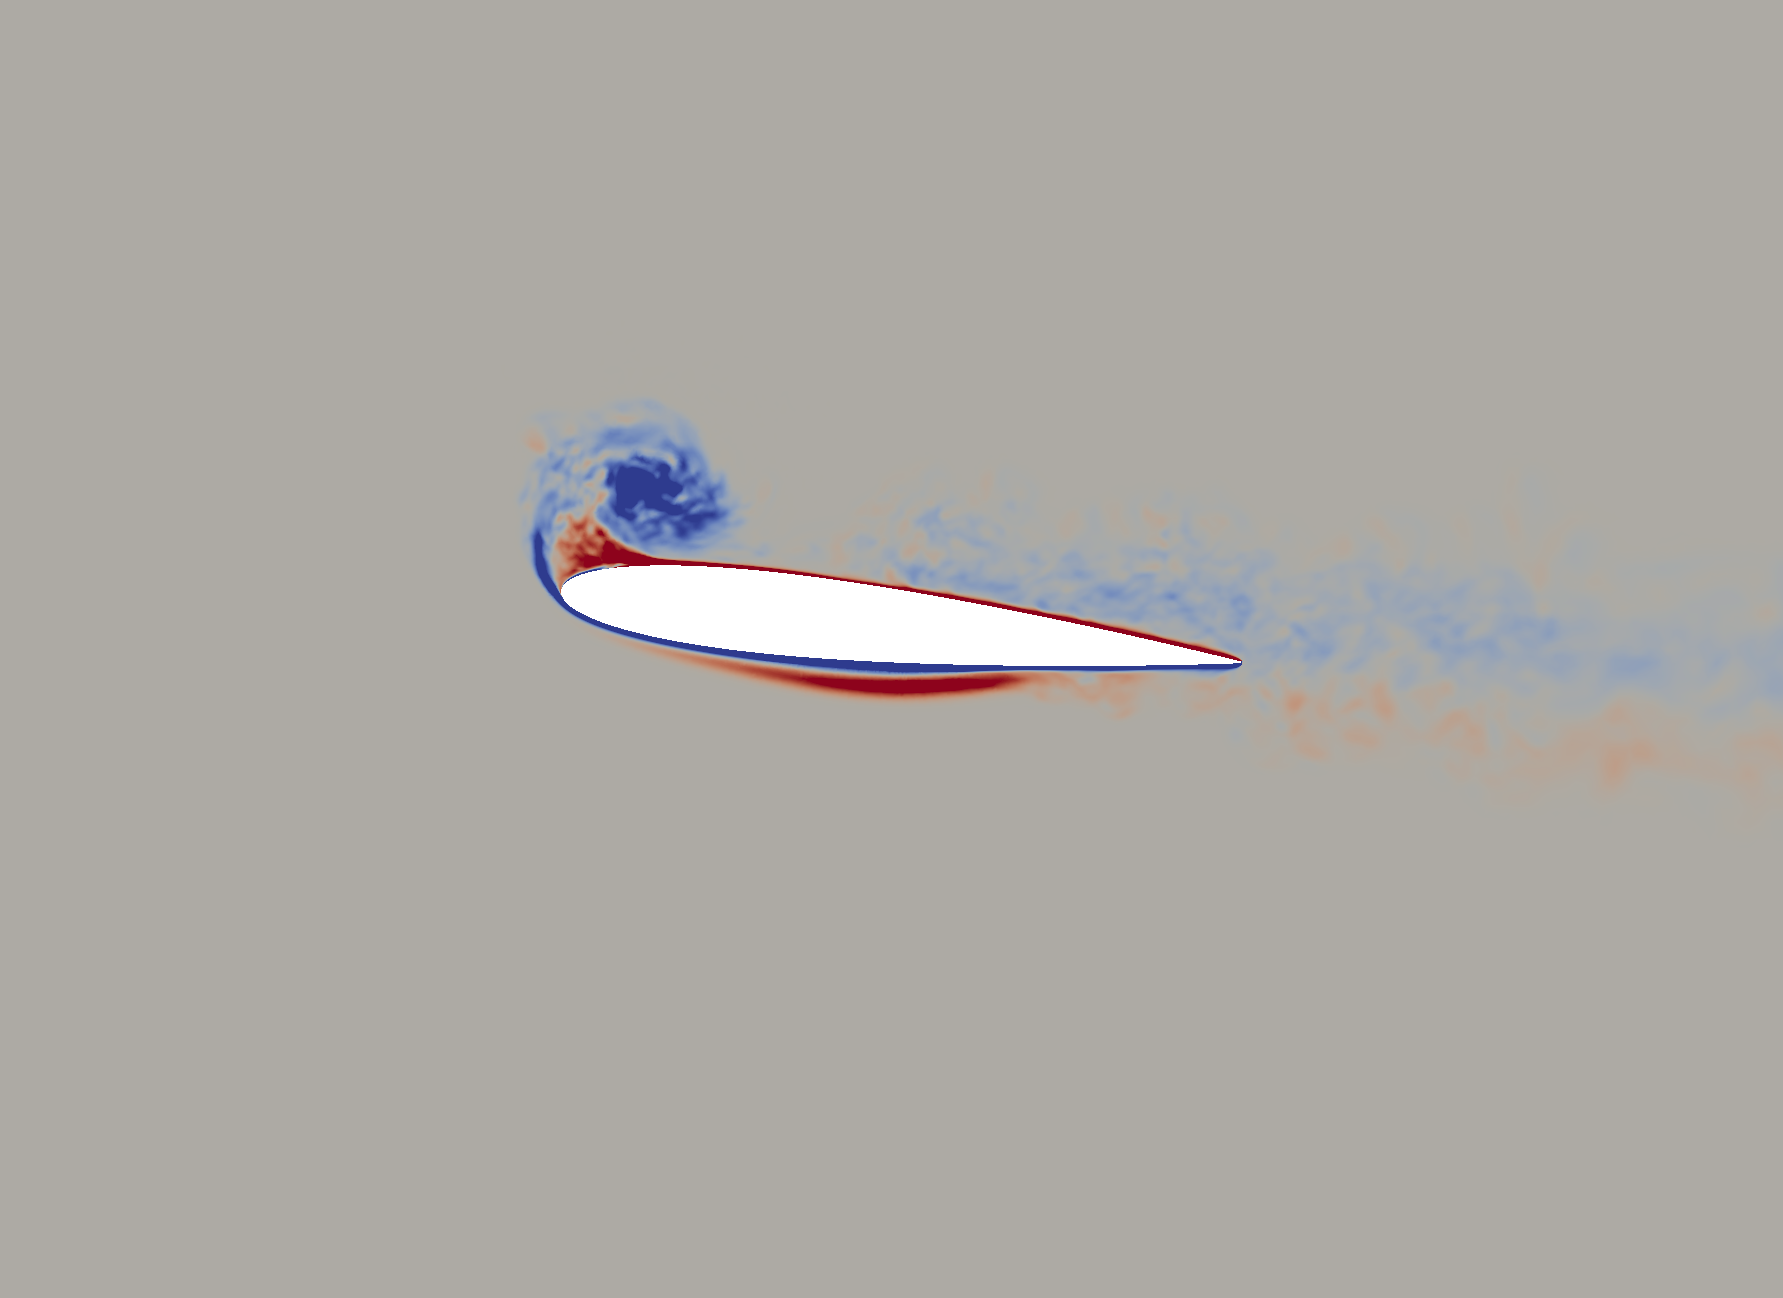
\includegraphics[width=1\textwidth]{figures/Vorticity_plots/Re_40k_1pt2/phase_240.png}
		\caption{$Re=4e4$, $\psi$ = $240^\circ$, $\tilde{t}=0.667$}
		\label{fig:Re_40k_1pt2_phi240}
	\end{subfigure}
	\begin{subfigure}[b]{0.32\textwidth}
		\centering
		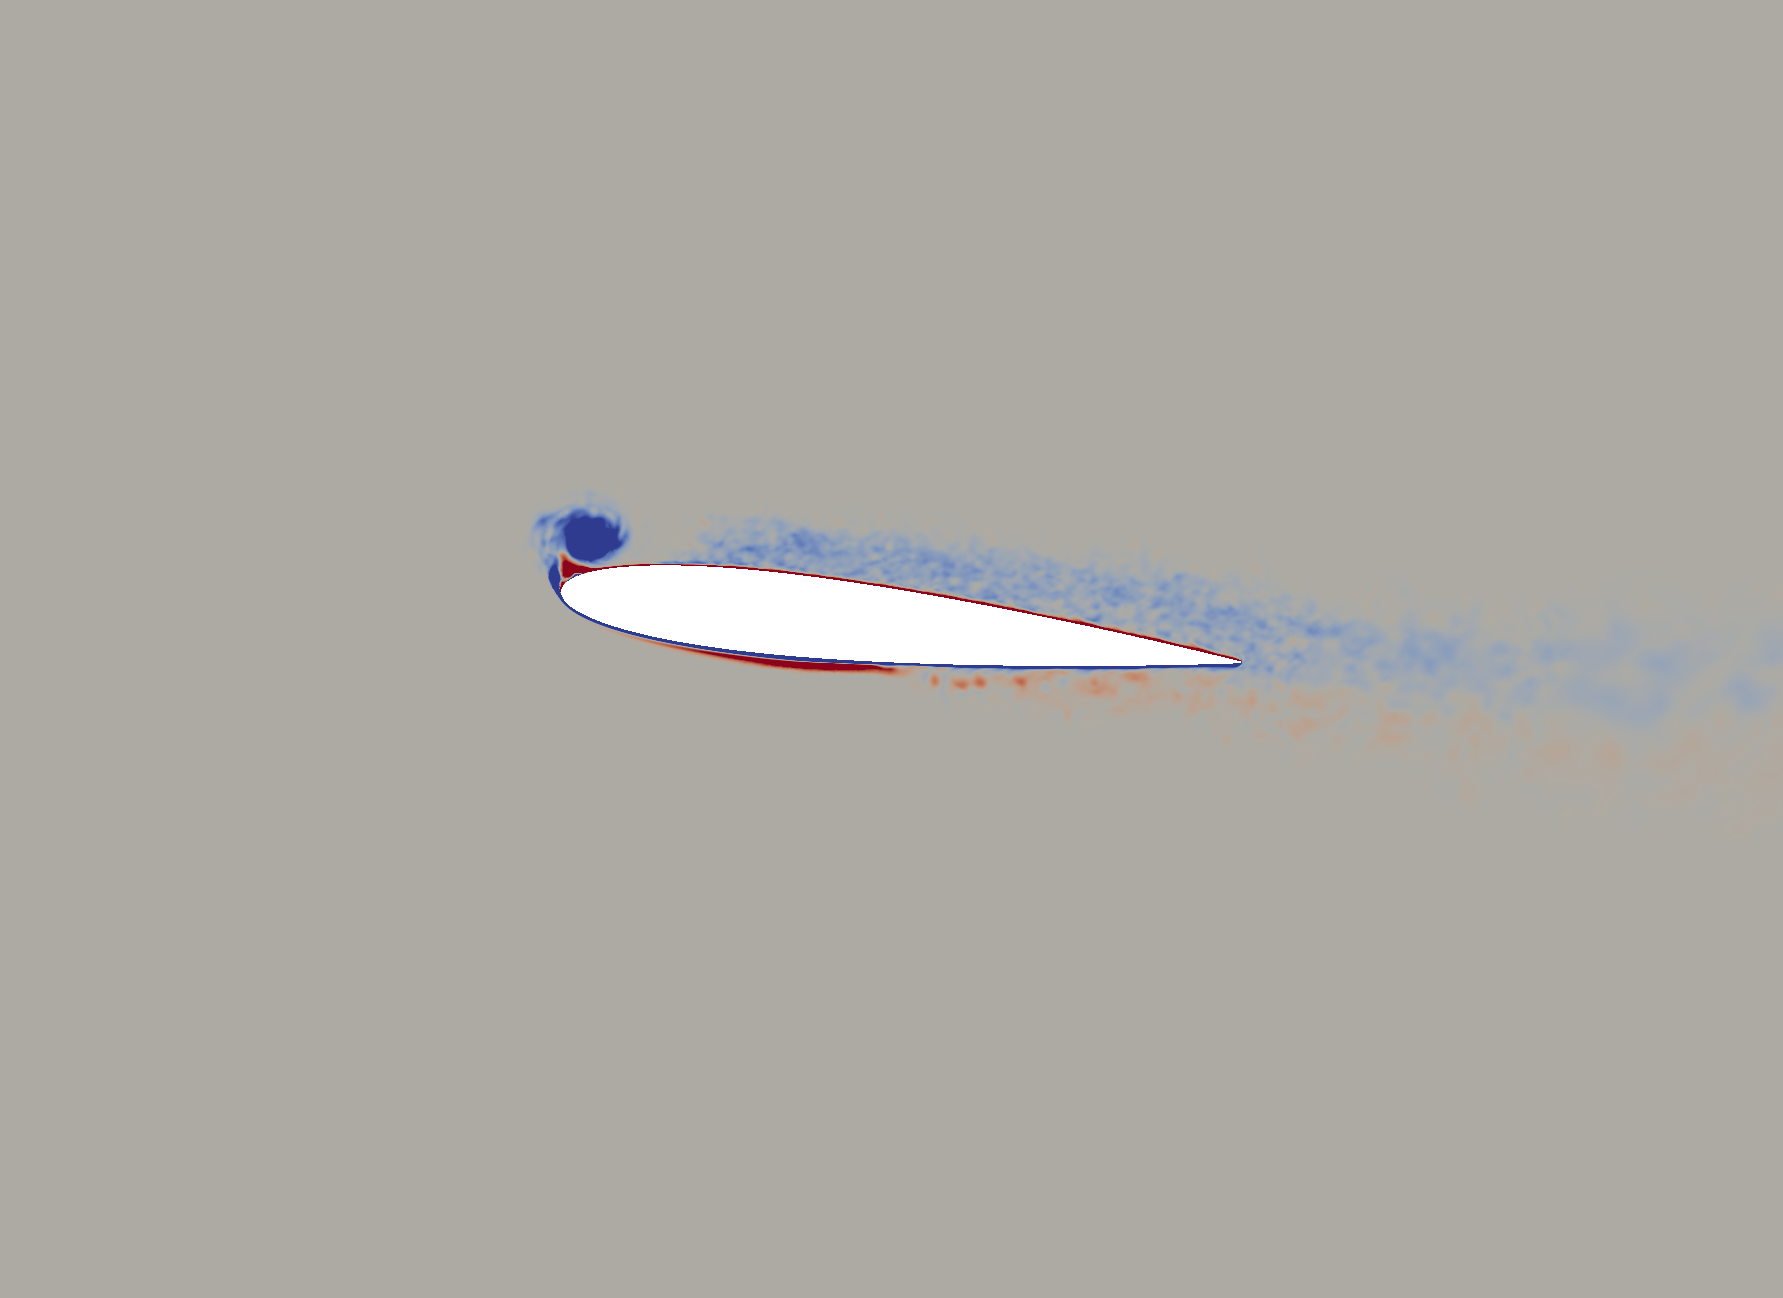
\includegraphics[width=1\textwidth]{figures/Vorticity_plots/Re_200k_1pt2/phase_240.png}
		\caption{$Re=2e5$, $\psi$ = $240^\circ$, $\tilde{t}=0.667$}
		\label{fig:Re_200k_1pt2_phi240}
	\end{subfigure}
	\begin{subfigure}[b]{0.32\textwidth}
		\centering
		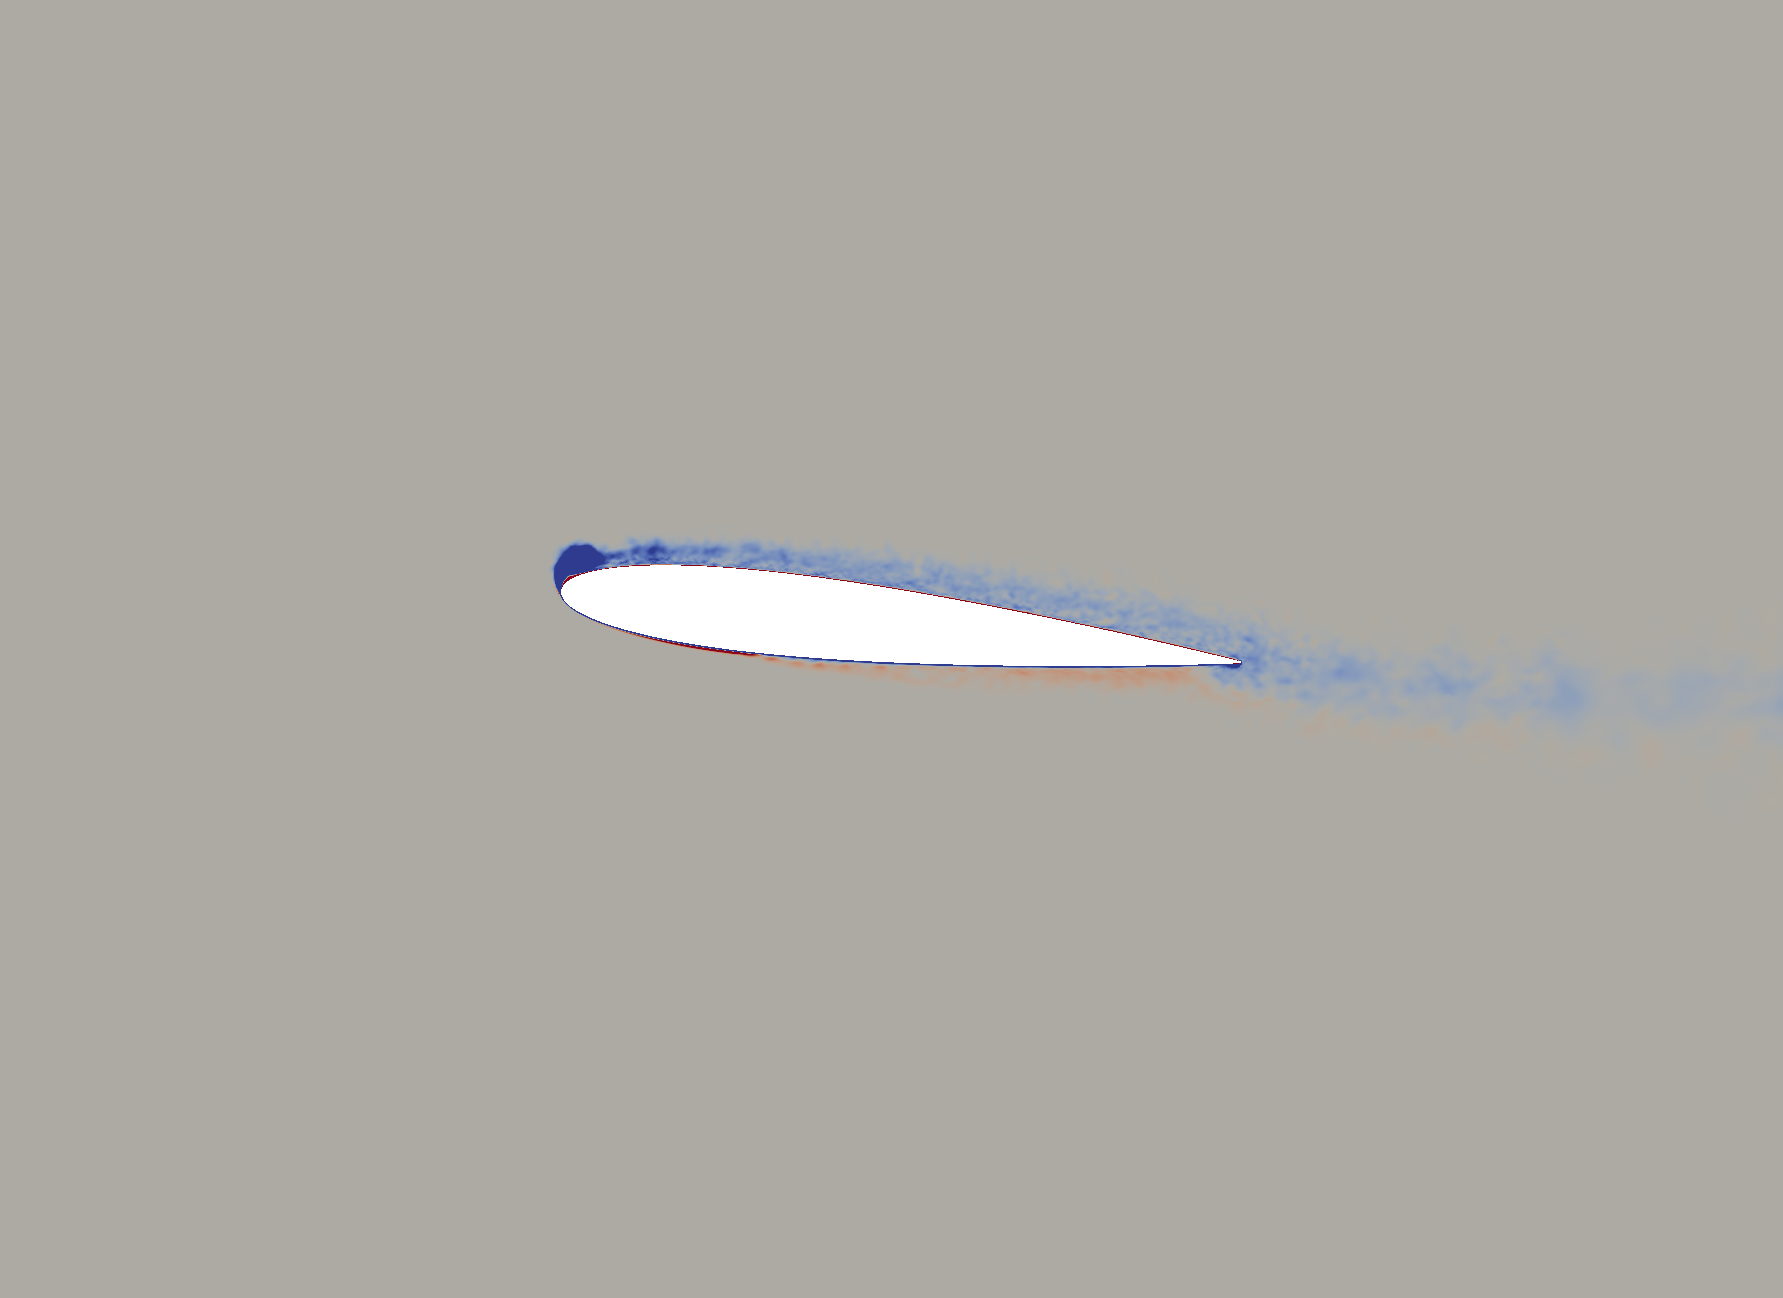
\includegraphics[width=1\textwidth]{figures/Vorticity_plots/Re_1m_1pt2/phase_240.png}
		\caption{$Re=1e6$, $\psi$ = $240^\circ$, $\tilde{t}=0.667$}
		\label{fig:Re_1m_1pt2_phi240}
	\end{subfigure}
	
	\begin{subfigure}[b]{0.32\textwidth}
		\centering
		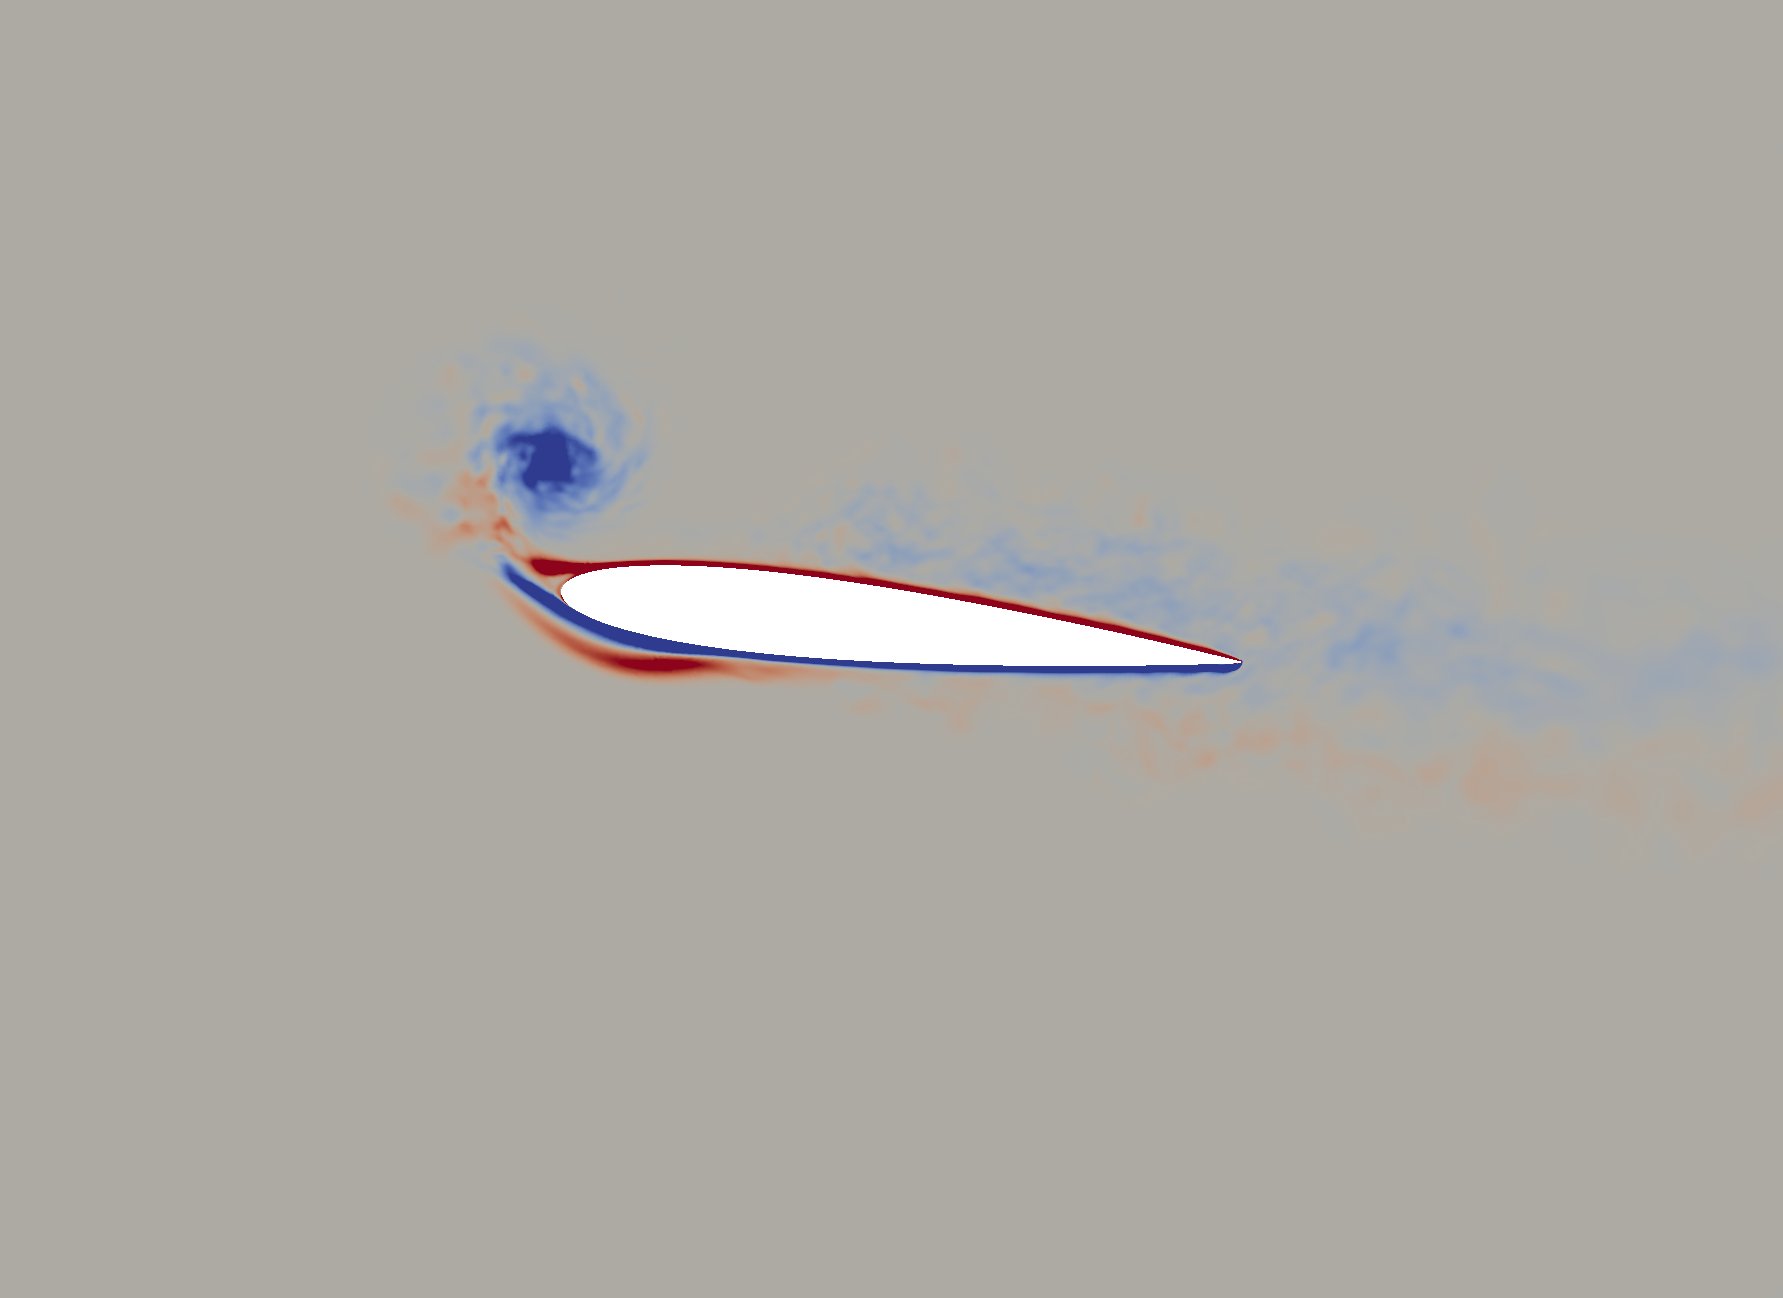
\includegraphics[width=1\textwidth]{figures/Vorticity_plots/Re_40k_1pt2/phase_255.png}
		\caption{$Re=4e4$, $\psi$ = $255^\circ$, $\tilde{t}=0.708$}
		\label{fig:Re_40k_1pt2_phi255}
	\end{subfigure}
	\begin{subfigure}[b]{0.32\textwidth}
		\centering
		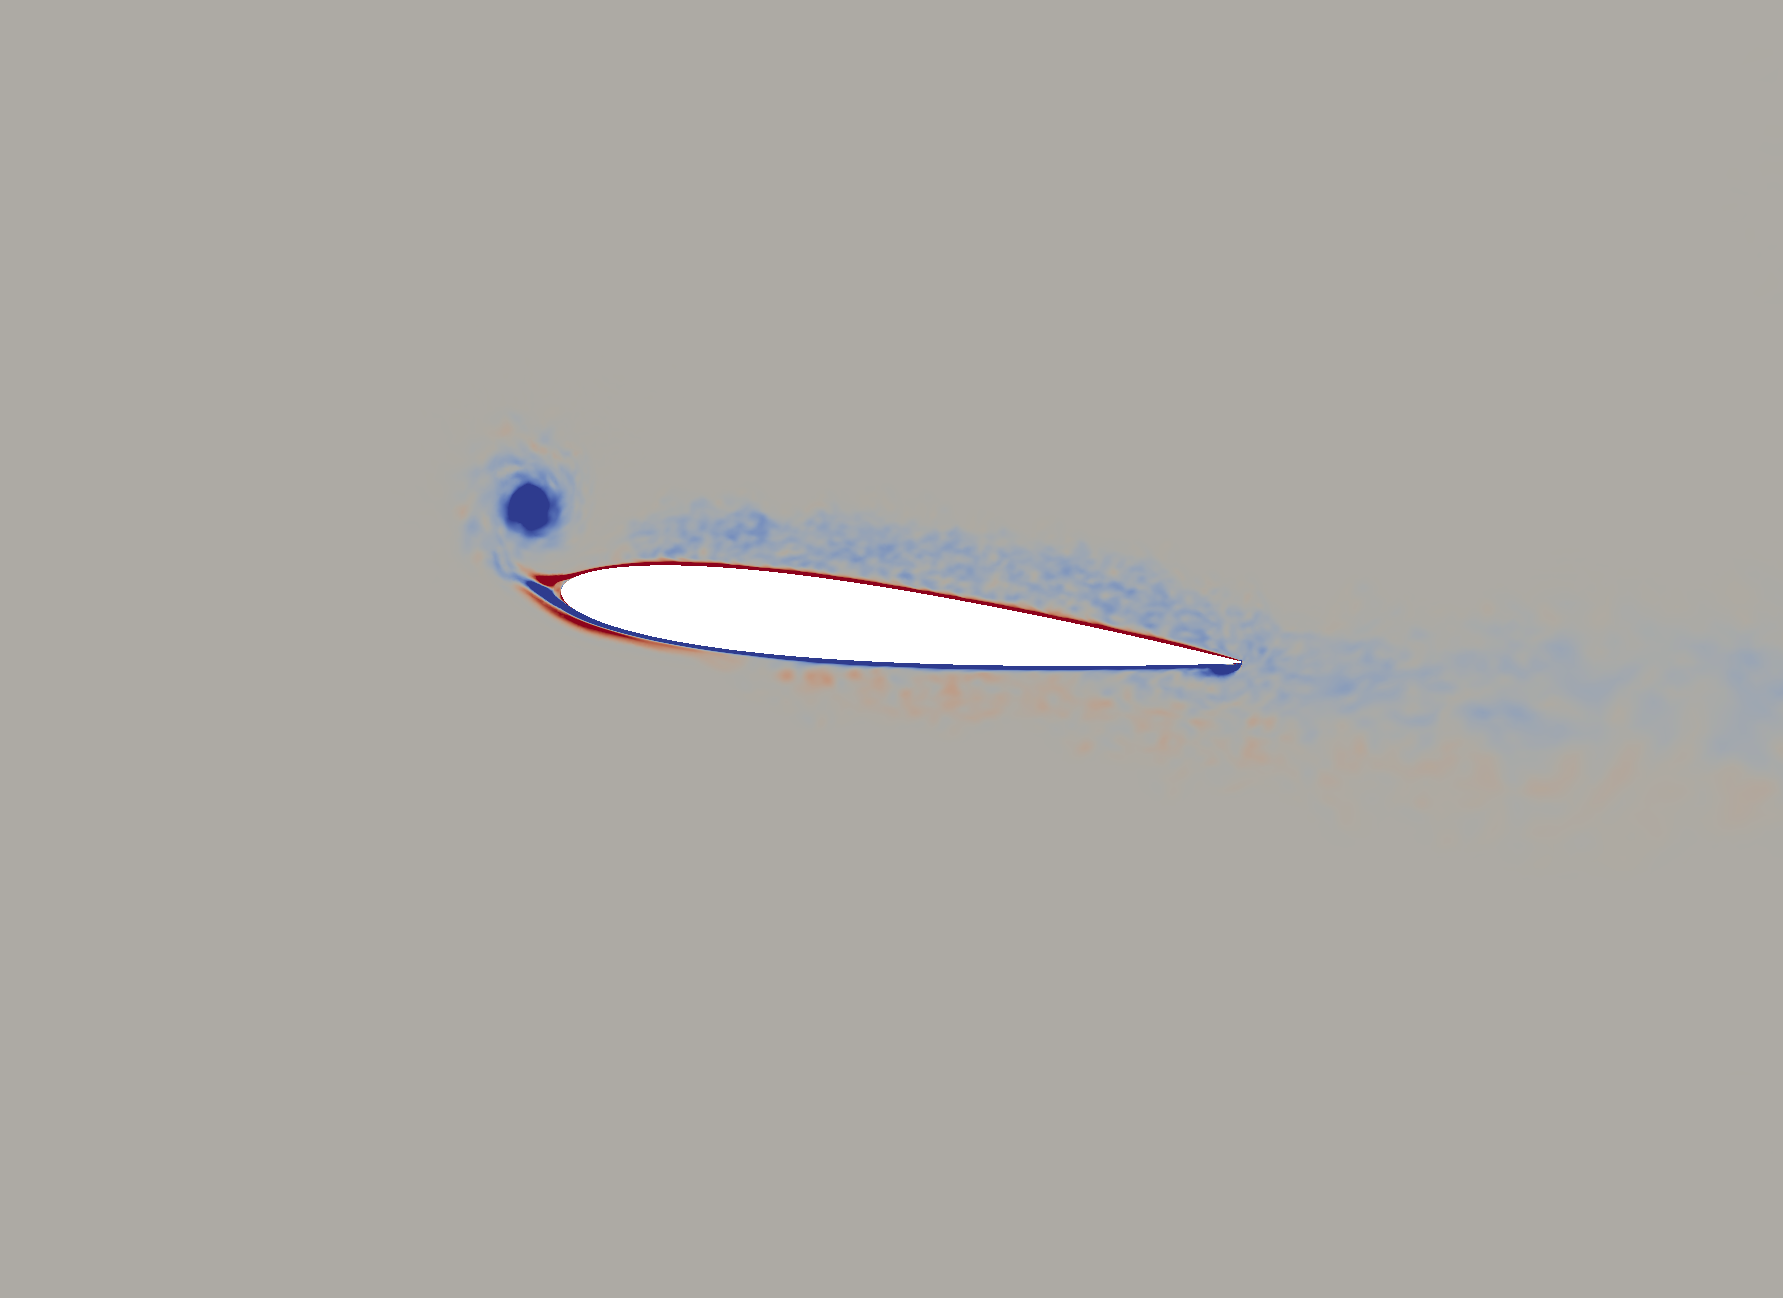
\includegraphics[width=1\textwidth]{figures/Vorticity_plots/Re_200k_1pt2/phase_255.png}
		\caption{$Re=2e5$, $\psi$ = $255^\circ$, $\tilde{t}=0.708$}
		\label{fig:Re_200k_1pt2_phi255}
	\end{subfigure}
	\begin{subfigure}[b]{0.32\textwidth}
		\centering
		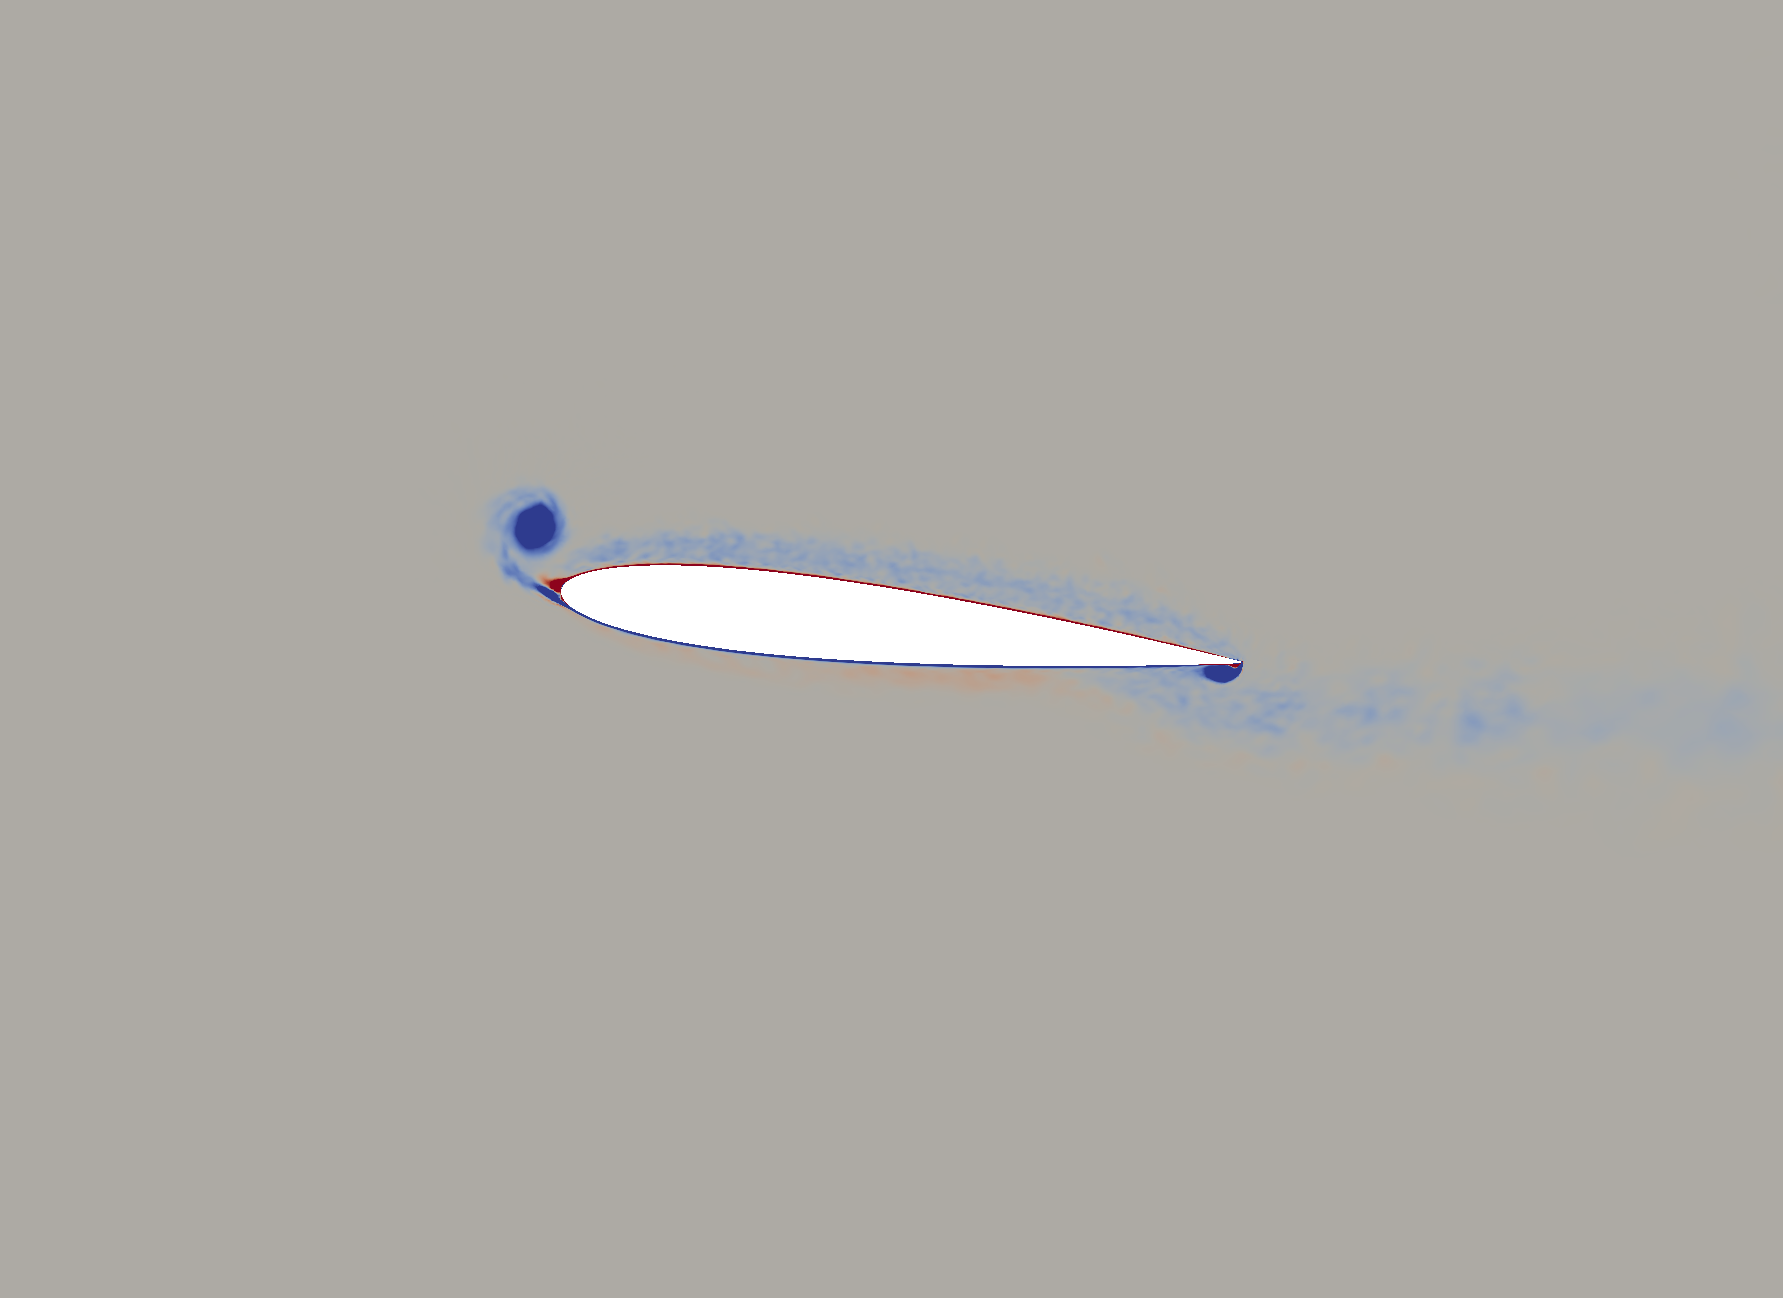
\includegraphics[width=1\textwidth]{figures/Vorticity_plots/Re_1m_1pt2/phase_255.png}
		\caption{$Re=1e6$, $\psi$ = $255^\circ$, $\tilde{t}=0.708$}
		\label{fig:Re_1m_1pt2_phi255}
	\end{subfigure}
	
	\caption{Spanwise vorticity at 8 different phases for $Re$=40,000 (left column), 200,000 (middle column) and 1,000,000 (right column) at $\mu_{sect}$ = 1.2}
%	\label{fig:vortScreen_1pt2}
\end{figure}


\begin{figure}[H]\ContinuedFloat
	\centering
	\begin{subfigure}[b]{0.32\textwidth}
		\centering
		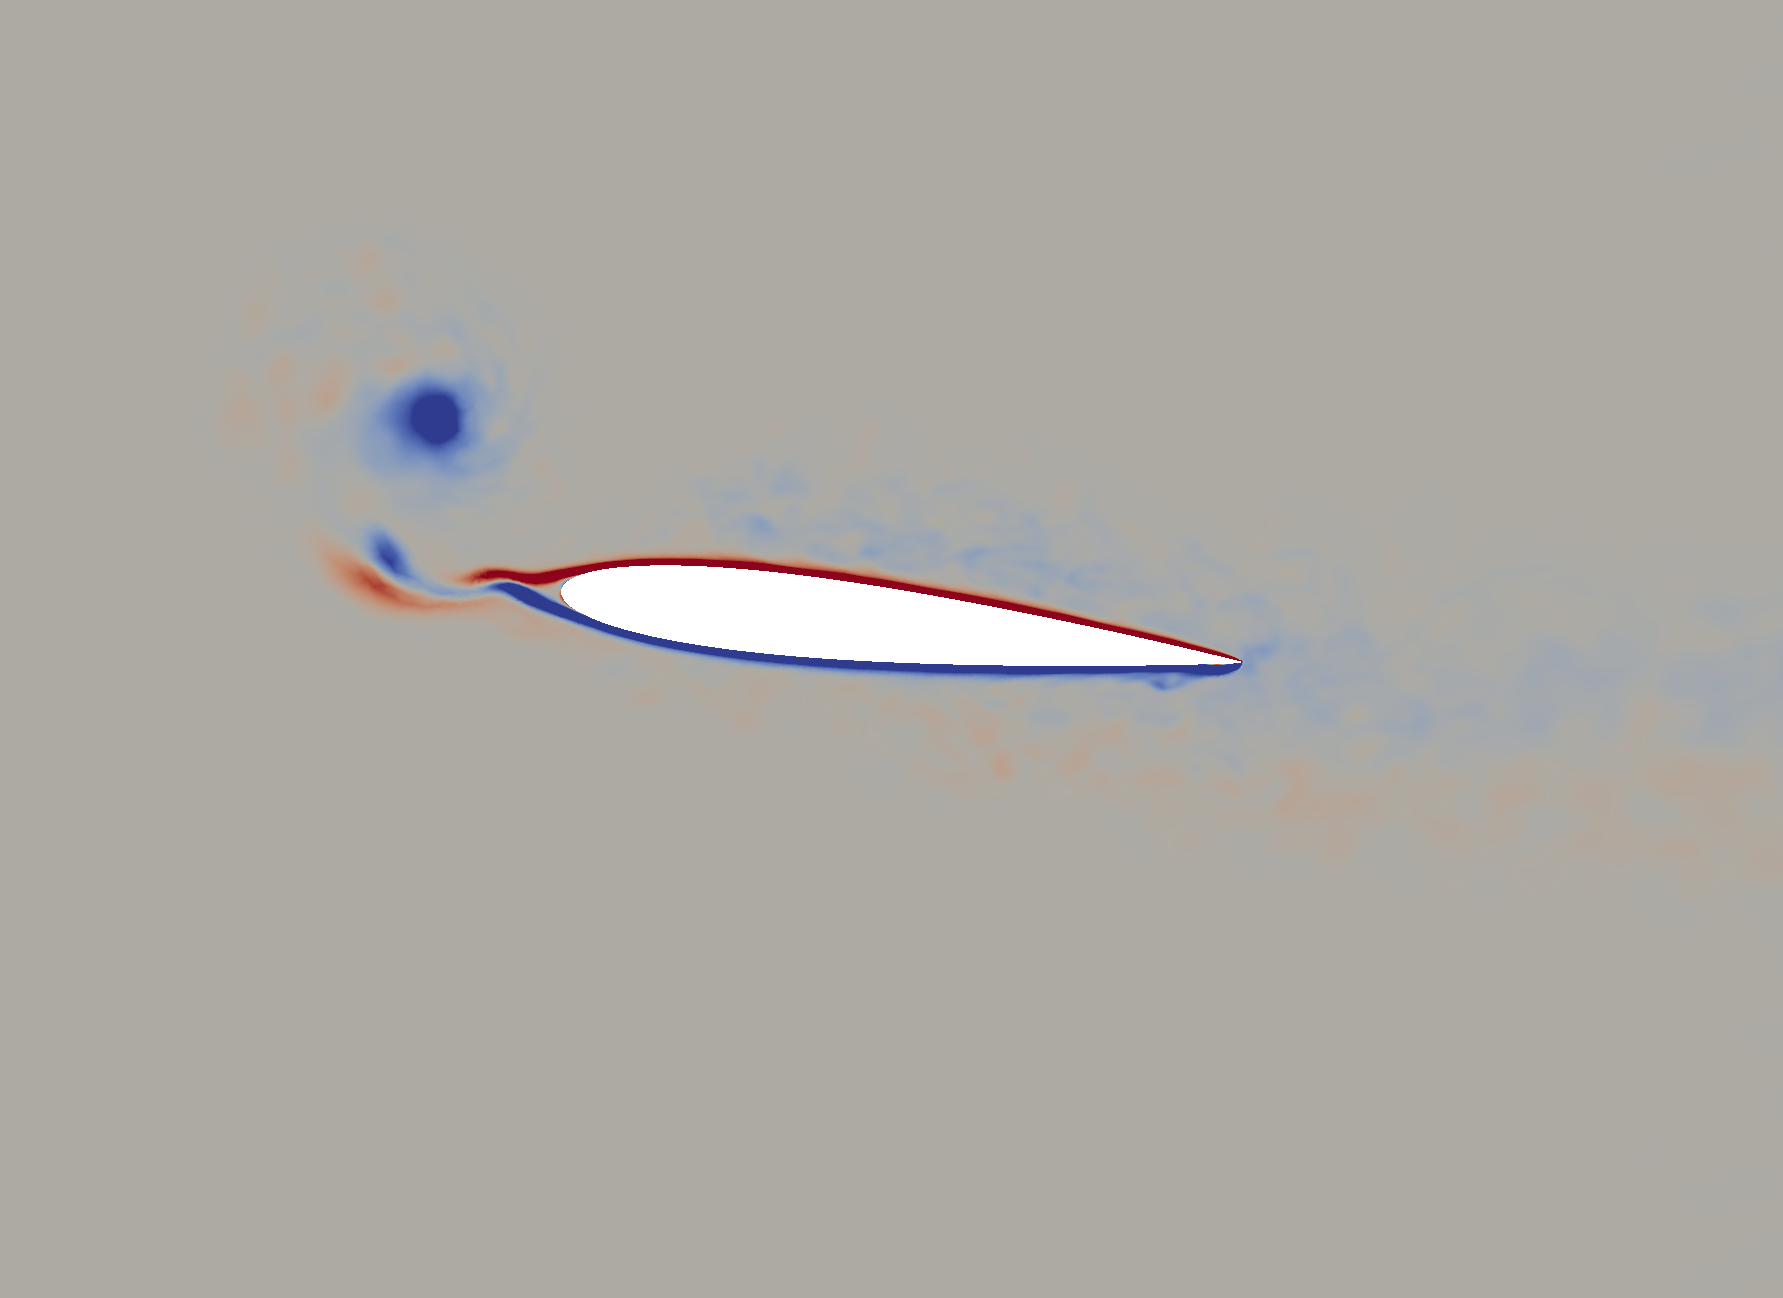
\includegraphics[width=1\textwidth]{figures/Vorticity_plots/Re_40k_1pt2/phase_270.png}
		\caption{$Re=4e4$, $\psi$ = $270^\circ$, $\tilde{t}=0.750$}
		\label{fig:Re_40k_1pt2_phi270}
	\end{subfigure}
	\begin{subfigure}[b]{0.32\textwidth}
		\centering
		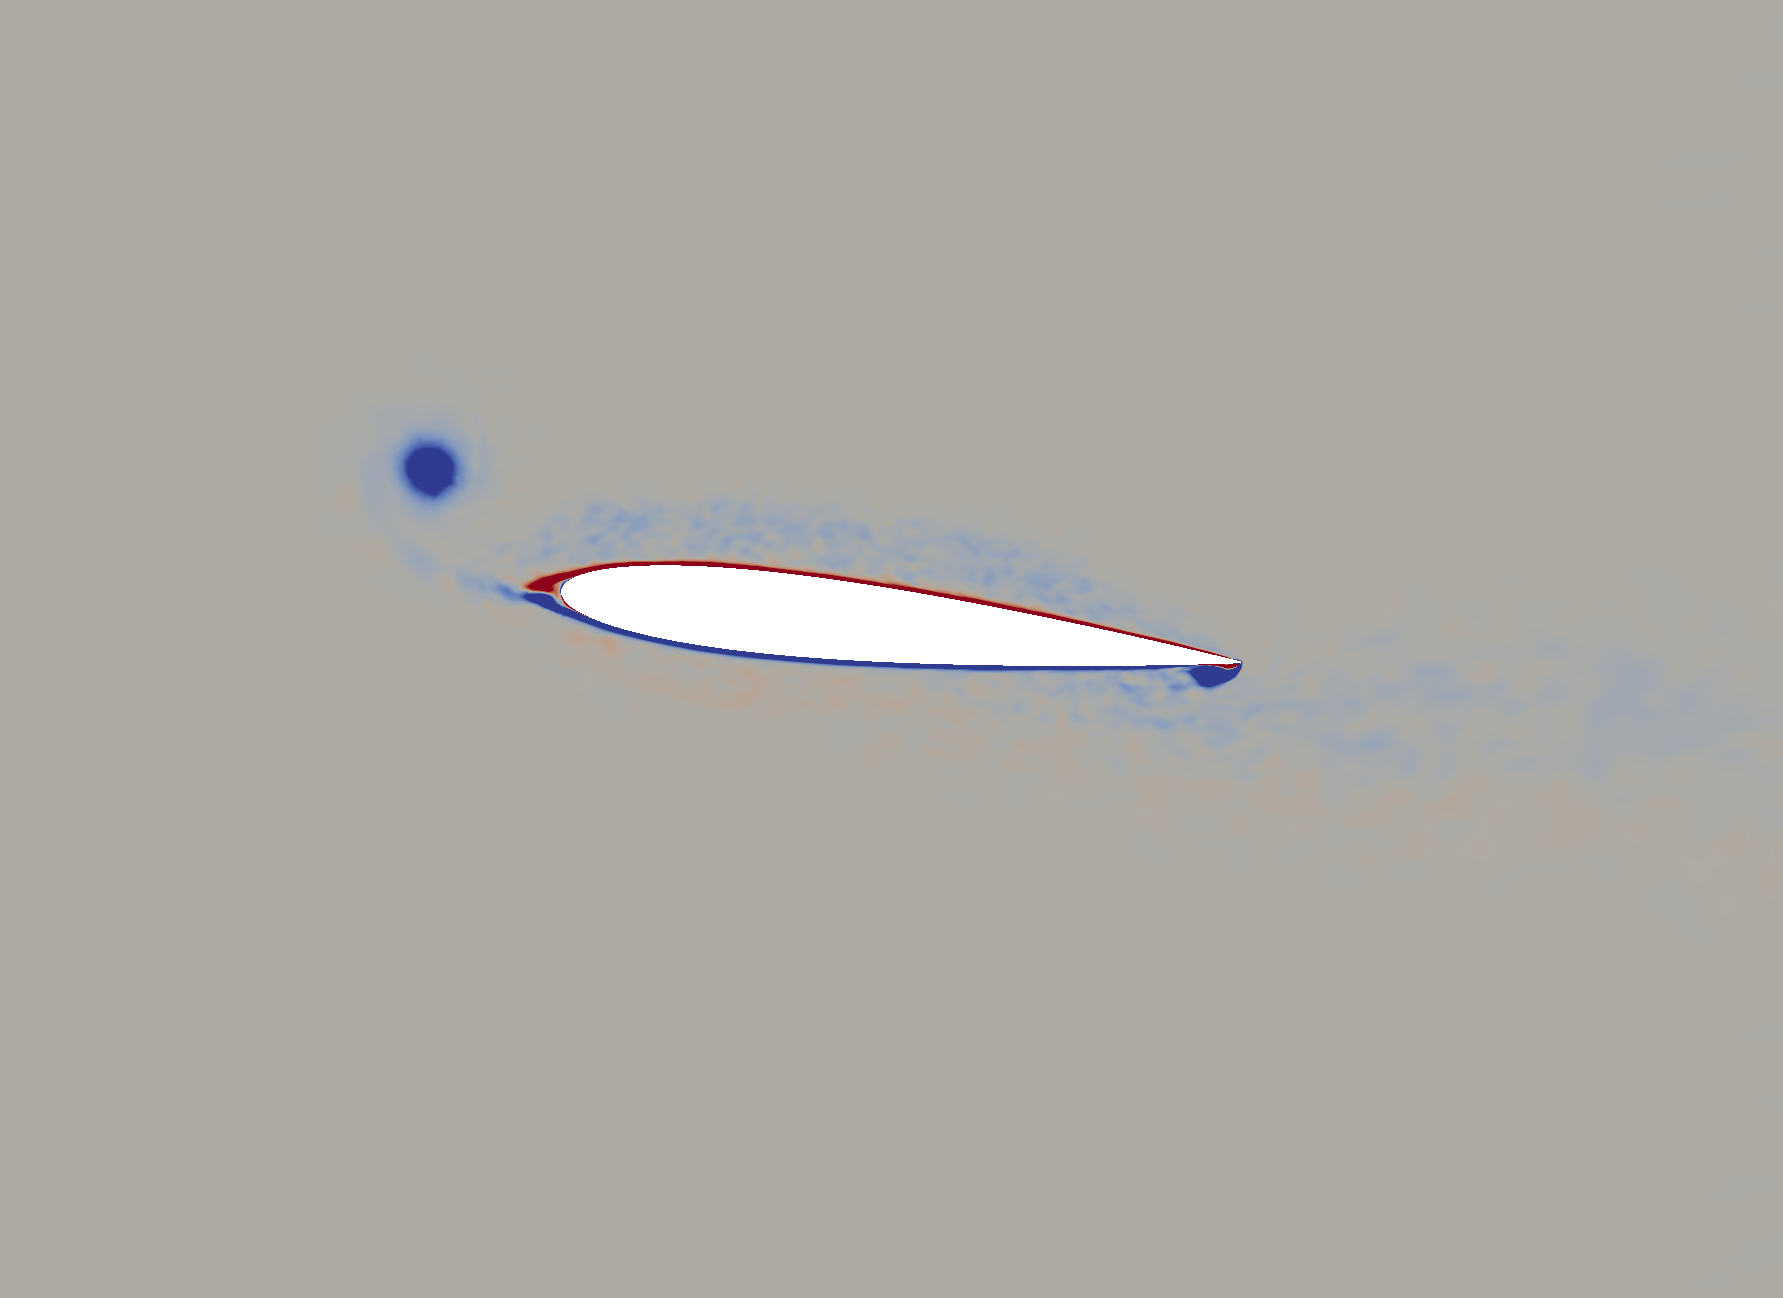
\includegraphics[width=1\textwidth]{figures/Vorticity_plots/Re_200k_1pt2/phase_270.png}
		\caption{$Re=2e5$, $\psi$ = $270^\circ$, $\tilde{t}=0.750$}
		\label{fig:Re_200k_1pt2_phi270}
	\end{subfigure}
	\begin{subfigure}[b]{0.32\textwidth}
		\centering
		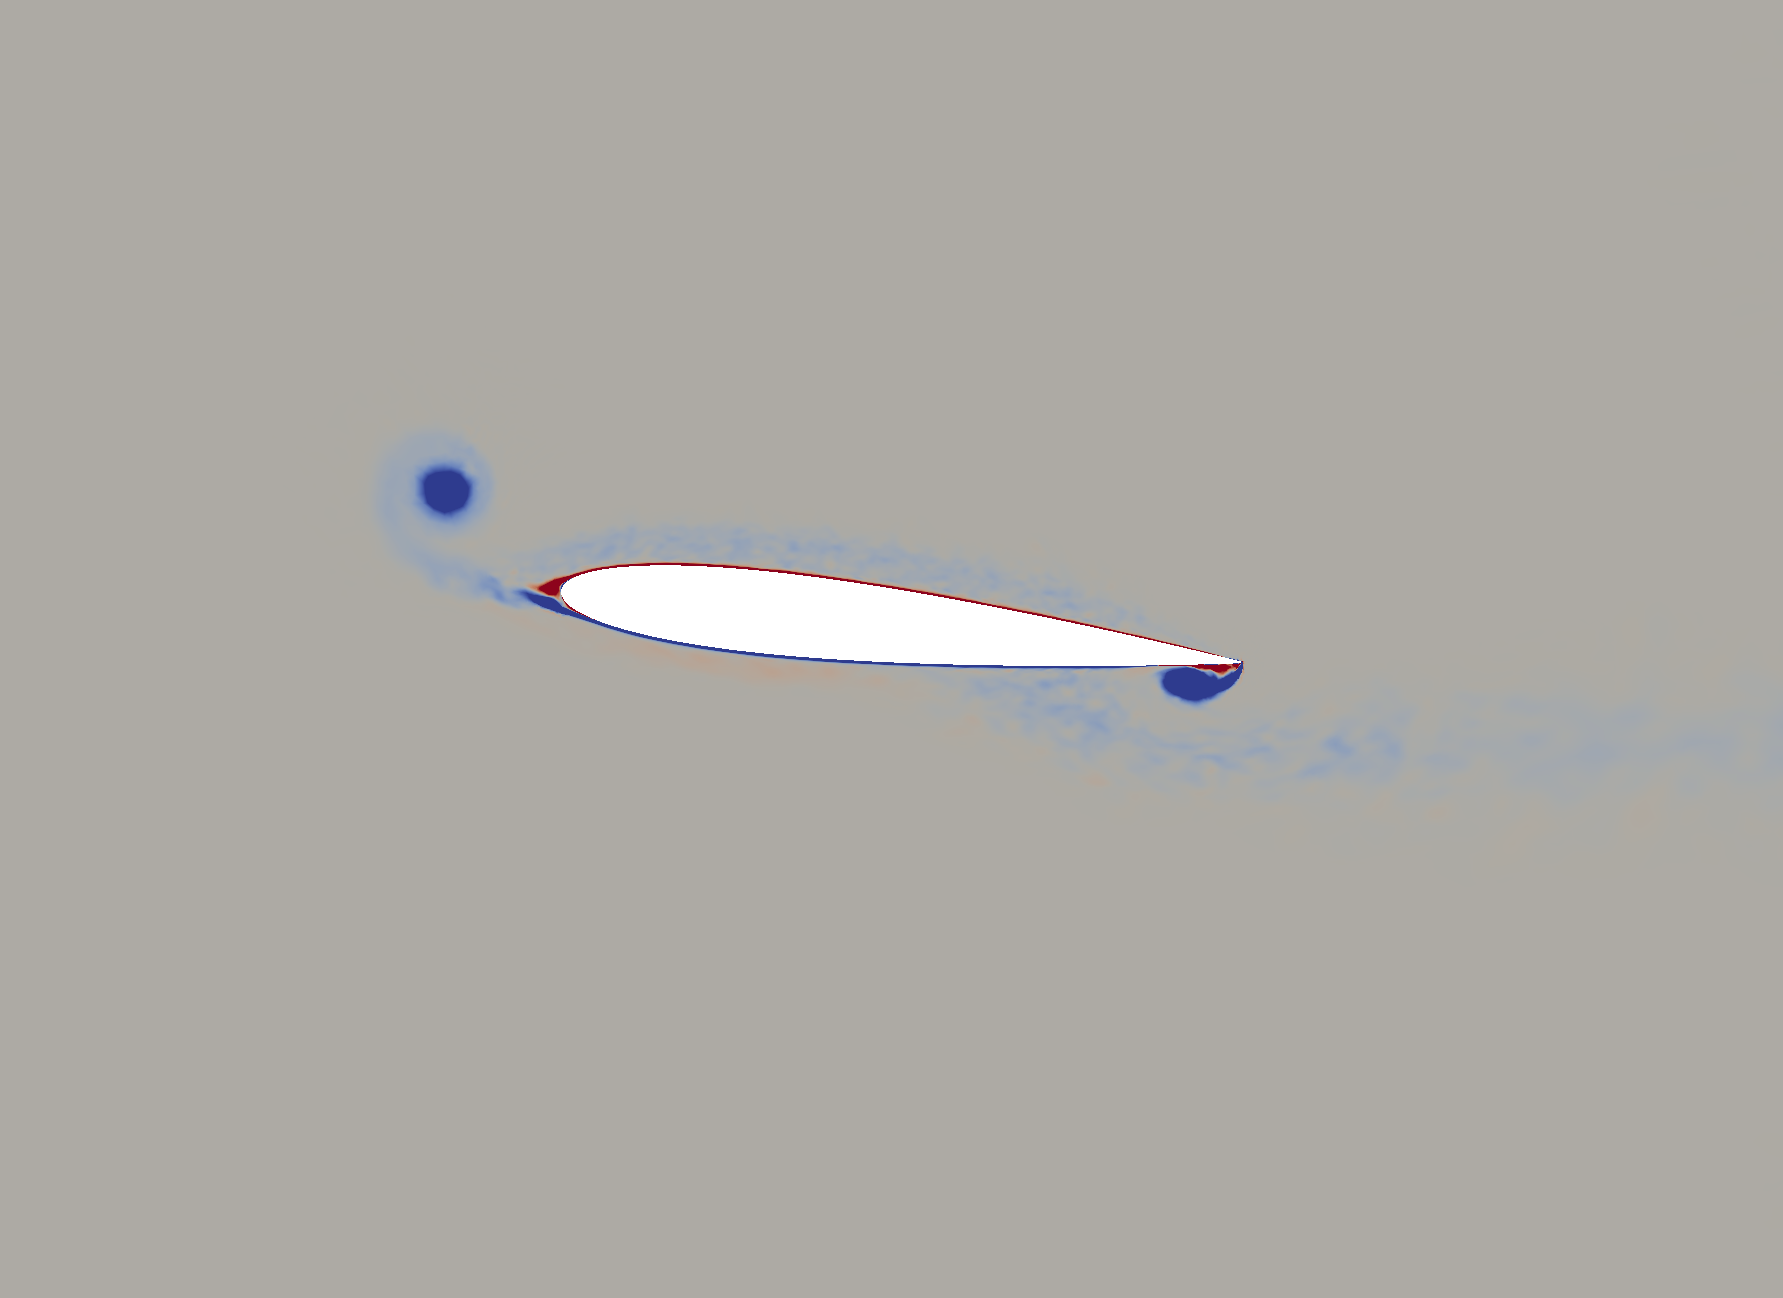
\includegraphics[width=1\textwidth]{figures/Vorticity_plots/Re_1m_1pt2/phase_270.png}
		\caption{$Re=1e6$, $\psi$ = $270^\circ$, $\tilde{t}=0.750$}
		\label{fig:Re_1m_1pt2_phi270}
	\end{subfigure}
	
	\begin{subfigure}[b]{0.32\textwidth}
		\centering
		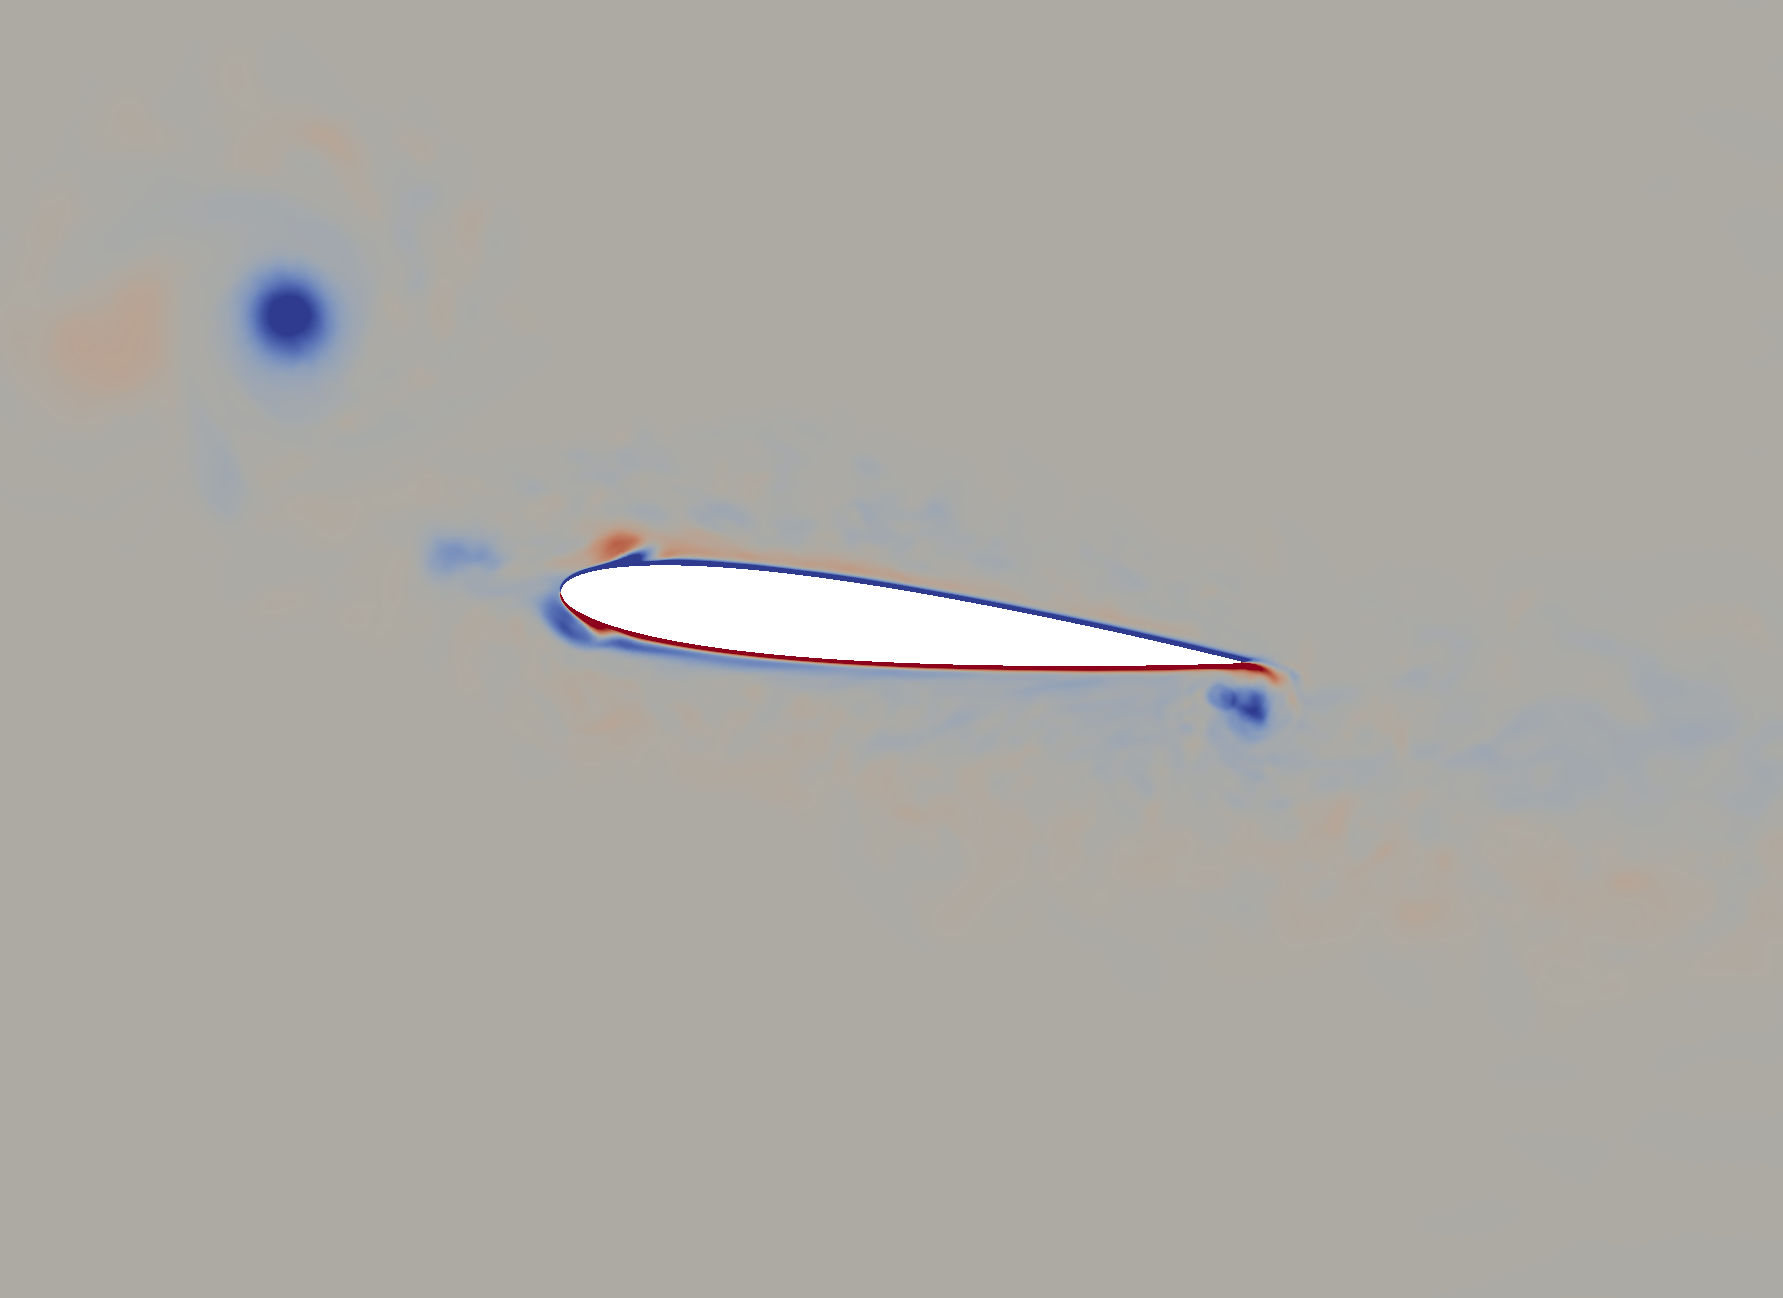
\includegraphics[width=1\textwidth]{figures/Vorticity_plots/Re_40k_1pt2/phase_315.png}
		\caption{$Re=4e4$, $\psi$ = $315^\circ$, $\tilde{t}=0.875$}
		\label{fig:Re_40k_1pt2_phi315}
	\end{subfigure}
	\begin{subfigure}[b]{0.32\textwidth}
		\centering
		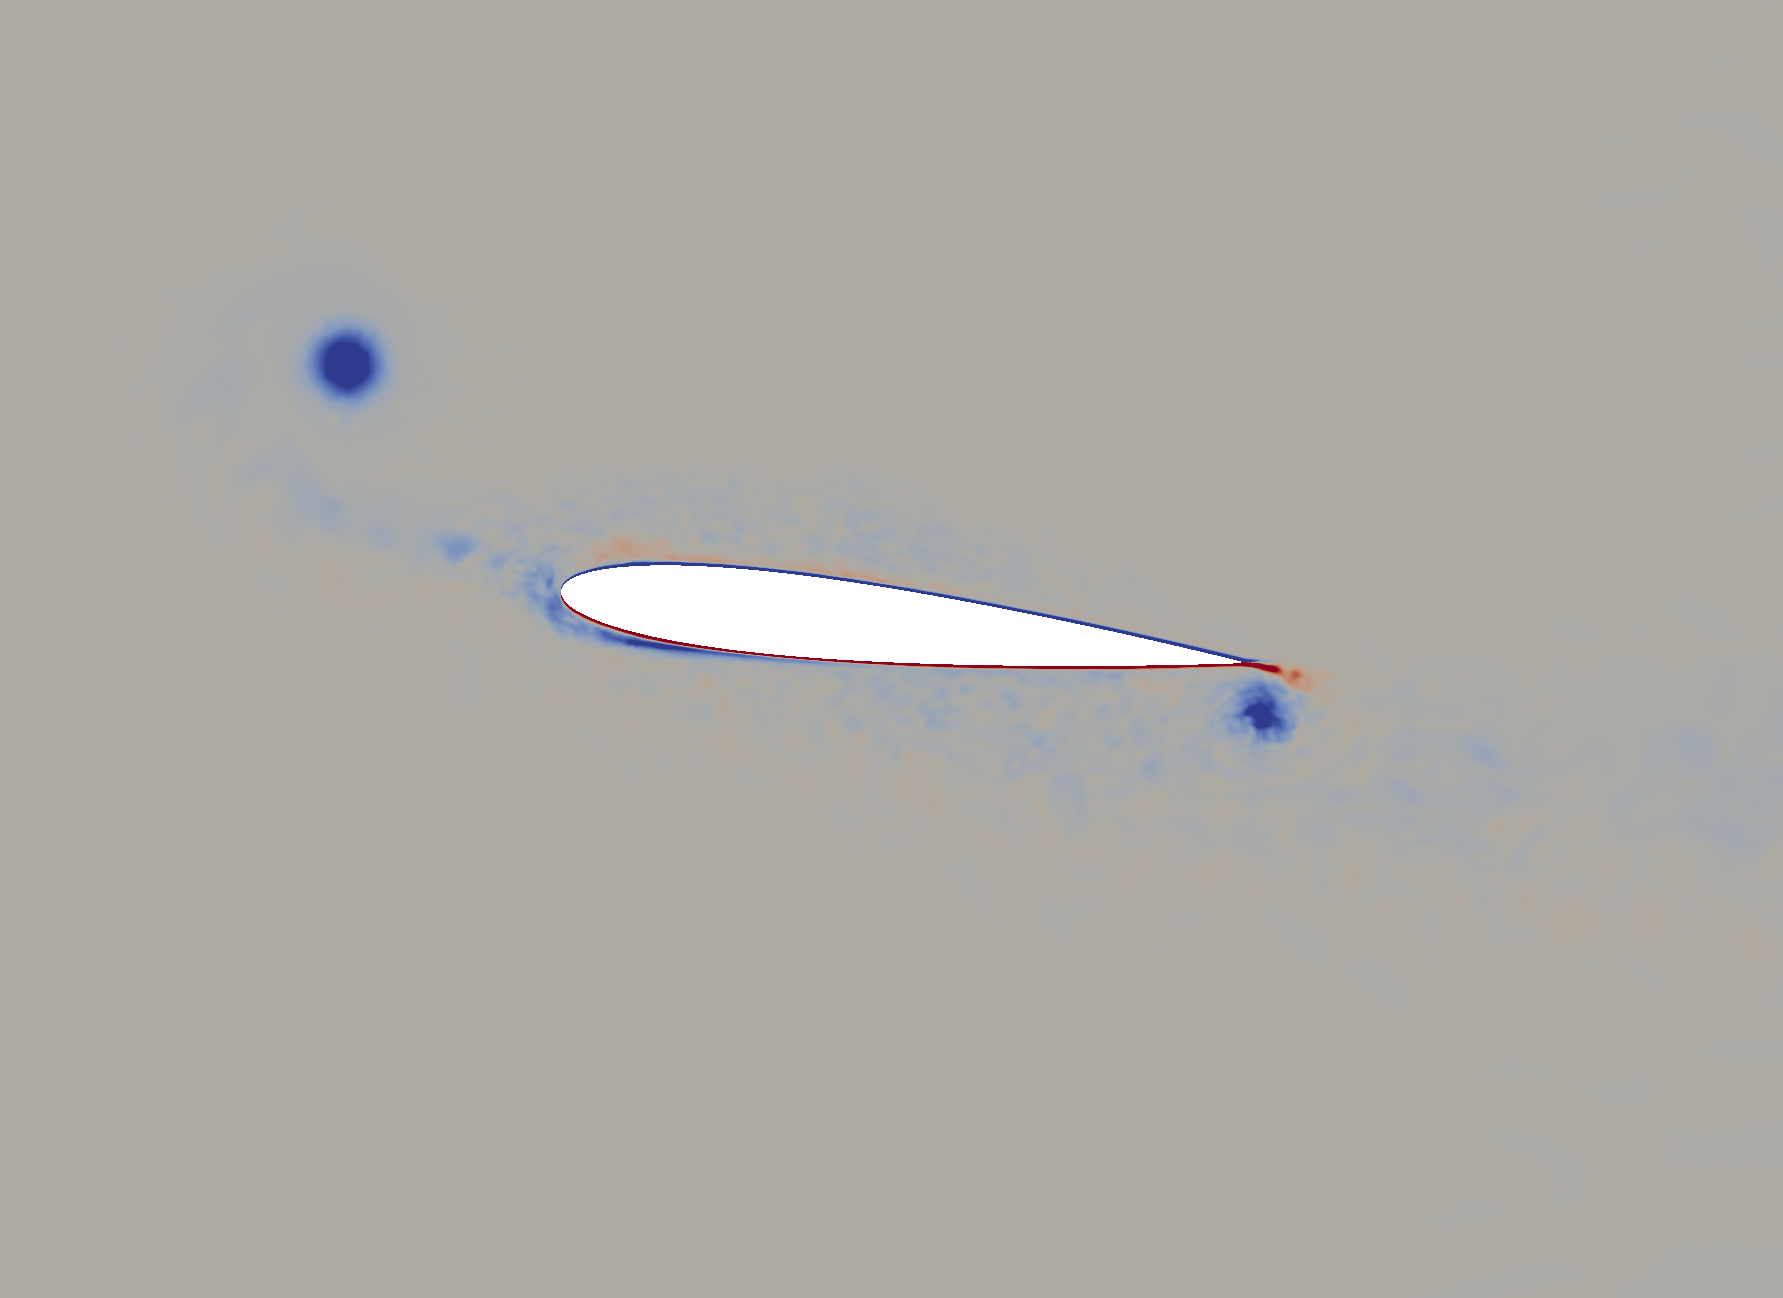
\includegraphics[width=1\textwidth]{figures/Vorticity_plots/Re_200k_1pt2/phase_315.png}
		\caption{$Re=2e5$, $\psi$ = $315^\circ$, $\tilde{t}=0.875$}
		\label{fig:Re_200k_1pt2_phi315}
	\end{subfigure}
	\begin{subfigure}[b]{0.32\textwidth}
		\centering
		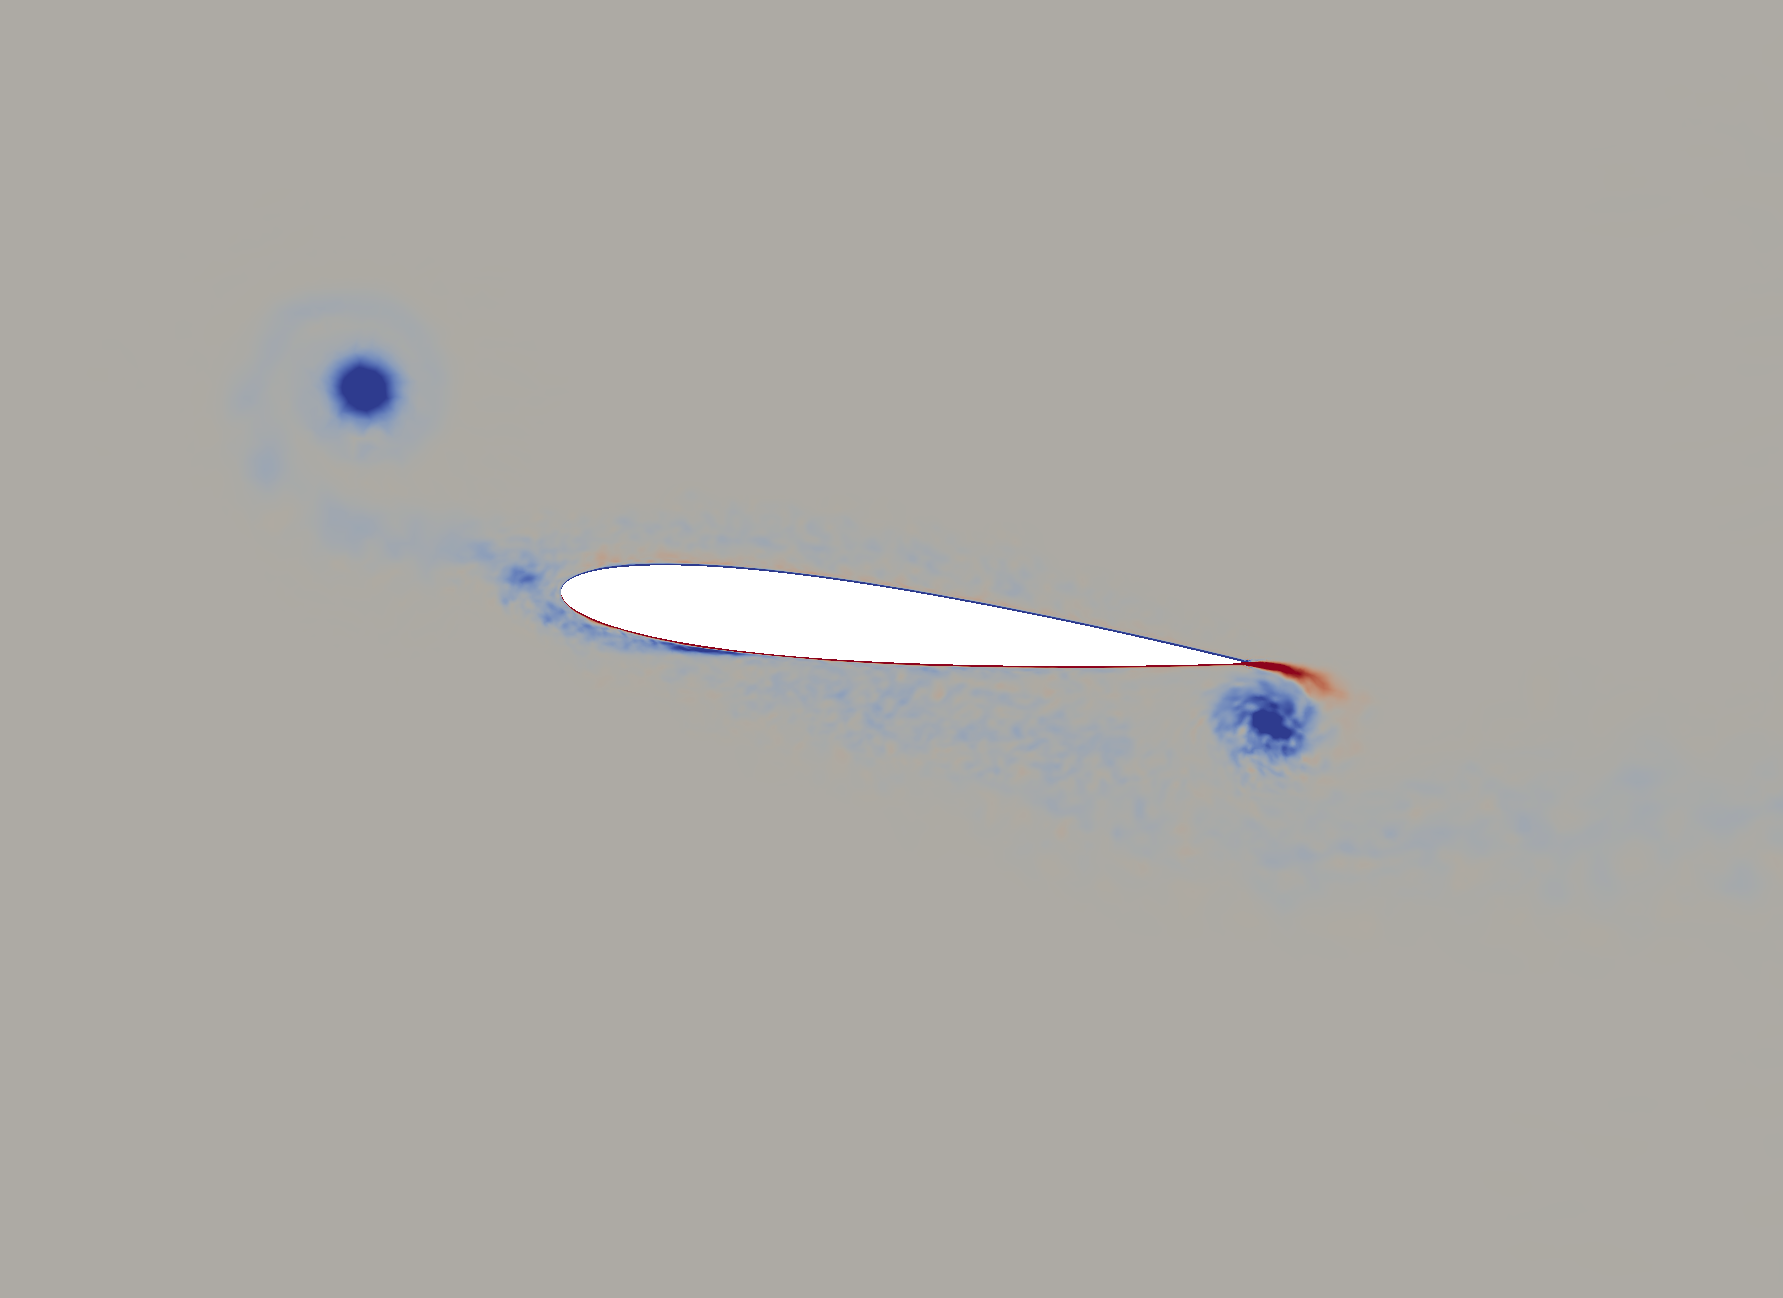
\includegraphics[width=1\textwidth]{figures/Vorticity_plots/Re_1m_1pt2/phase_315.png}
		\caption{$Re=1e6$, $\psi$ = $315^\circ$, $\tilde{t}=0.875$}
		\label{fig:Re_1m_1pt2_phi315}
	\end{subfigure}
	
	\begin{subfigure}[b]{0.32\textwidth}
		\centering
		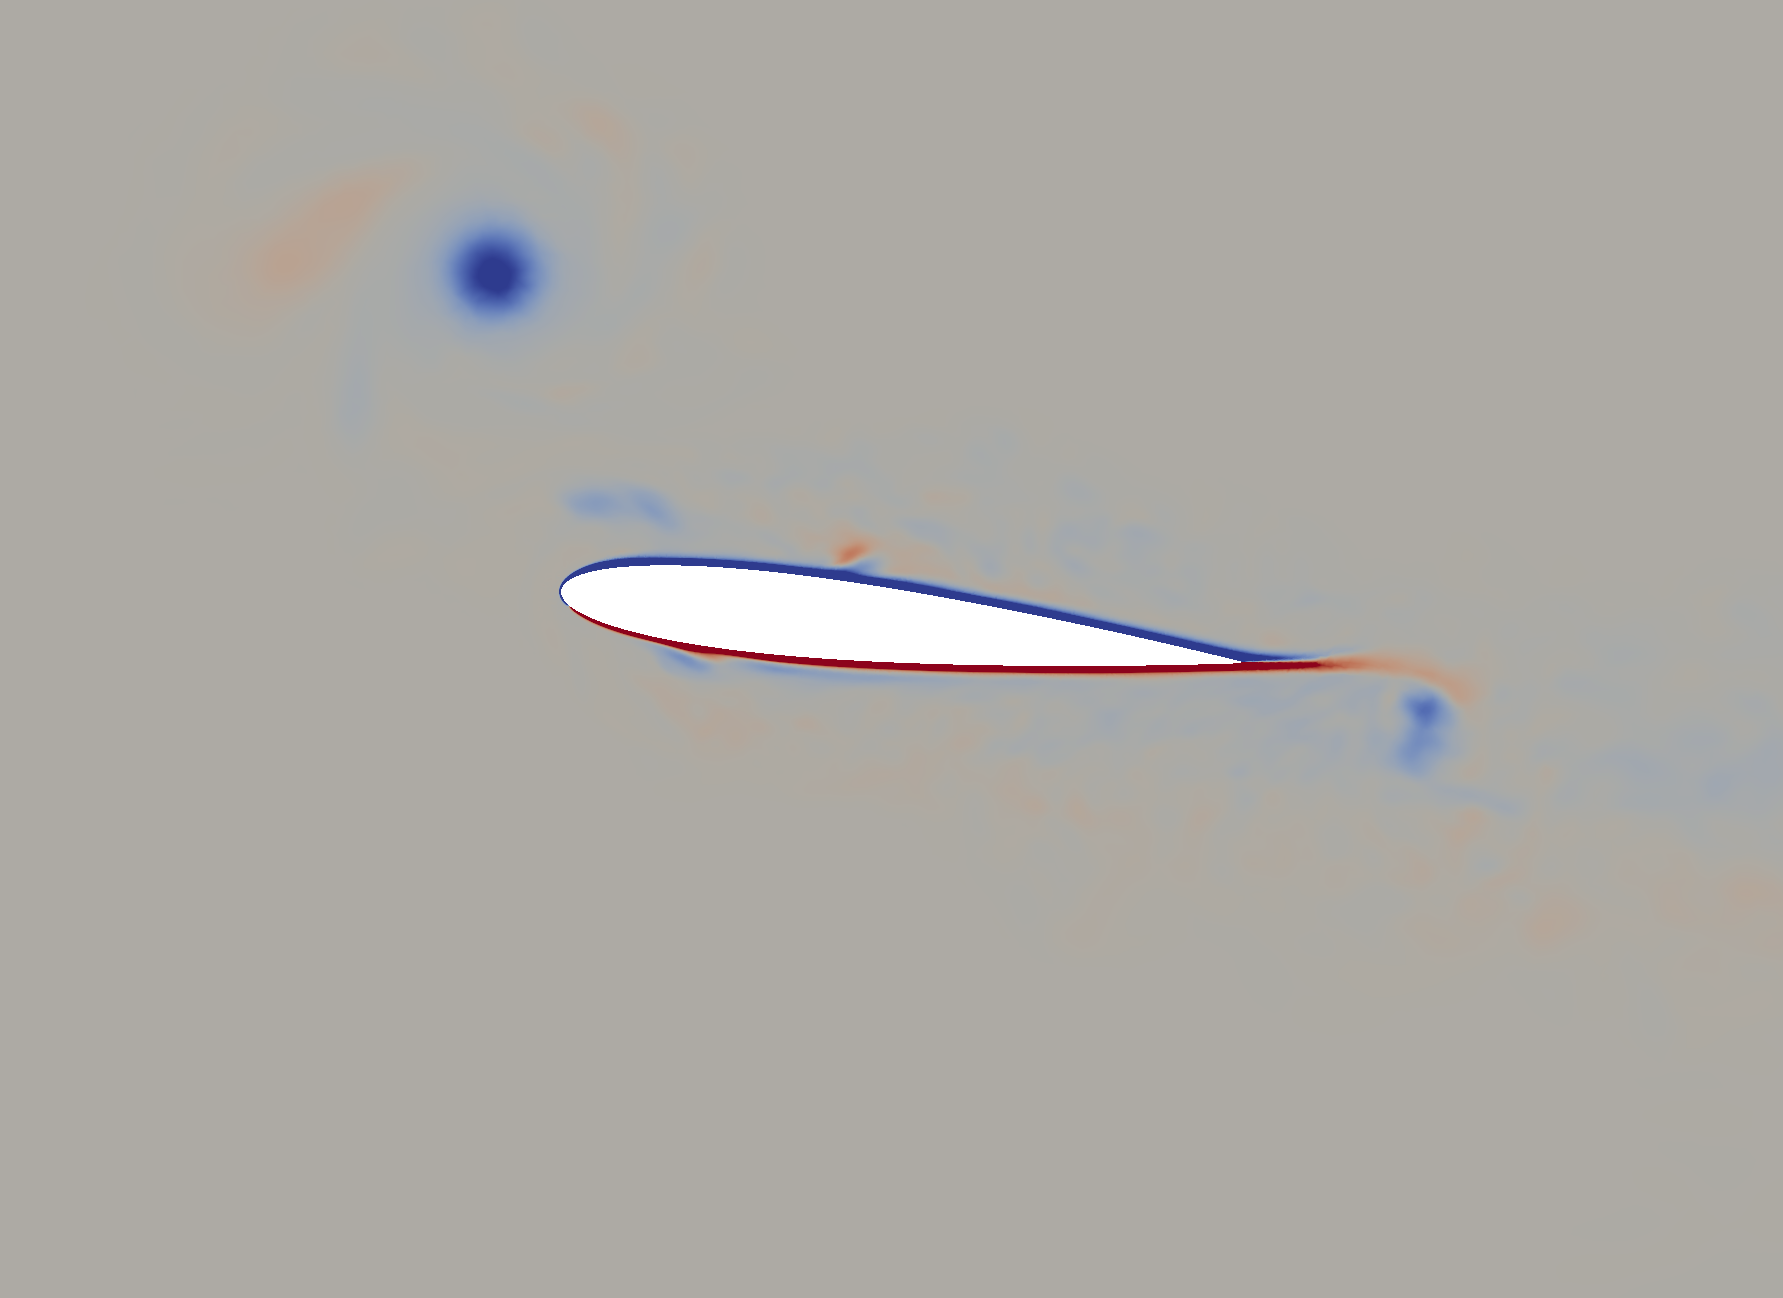
\includegraphics[width=1\textwidth]{figures/Vorticity_plots/Re_40k_1pt2/phase_330.png}
		\caption{$Re=4e4$, $\psi$ = $330^\circ$, $\tilde{t}=0.917$}
		\label{fig:Re_40k_1pt2_phi330}
	\end{subfigure}
	\begin{subfigure}[b]{0.32\textwidth}
		\centering
		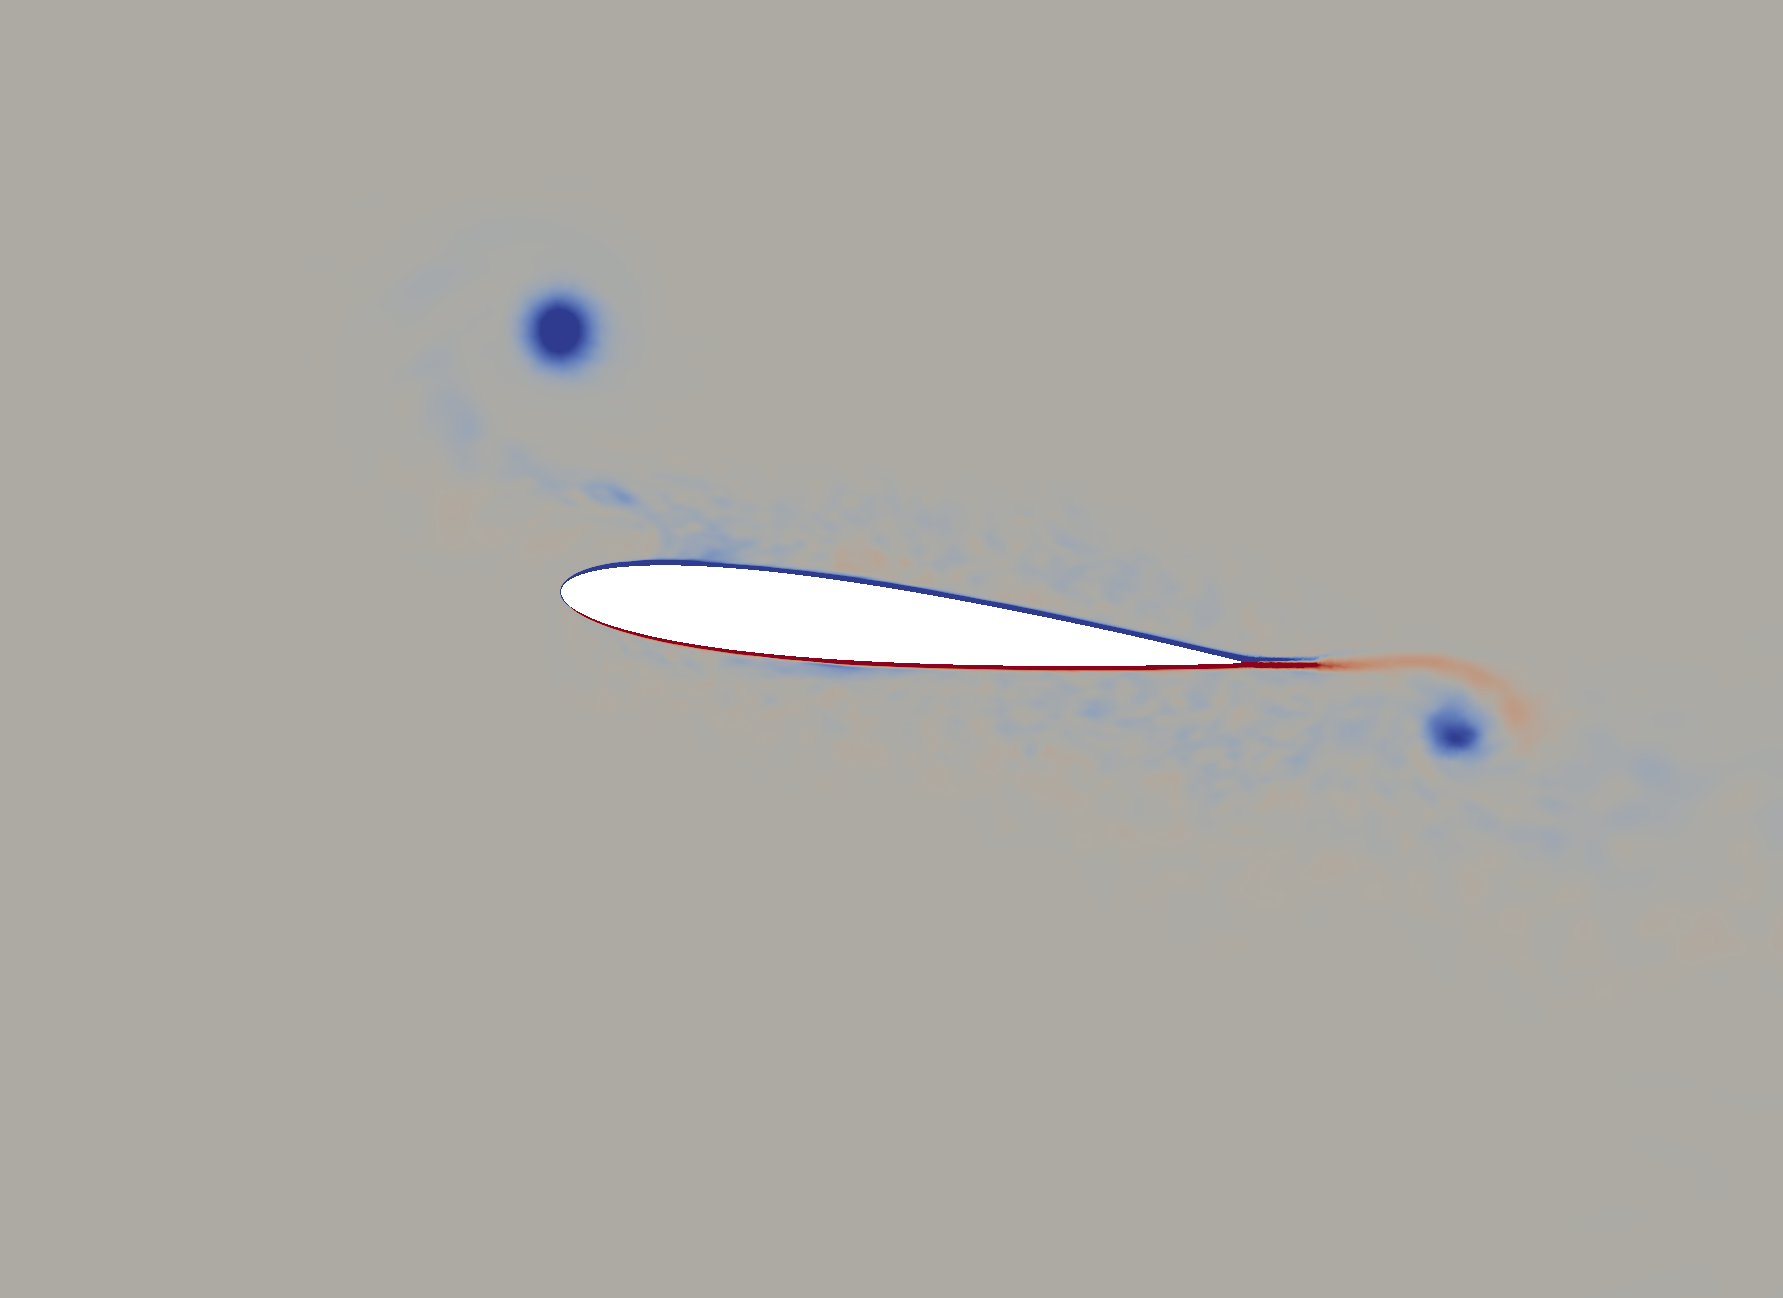
\includegraphics[width=1\textwidth]{figures/Vorticity_plots/Re_200k_1pt2/phase_330.png}
		\caption{$Re=2e5$, $\psi$ = $330^\circ$, $\tilde{t}=0.917$}
		\label{fig:Re_200k_1pt2_phi330}
	\end{subfigure}
	\begin{subfigure}[b]{0.32\textwidth}
		\centering
		\includegraphics[width=1\textwidth]{figures/Vorticity_plots/Re_1m_1pt2/phase_330.png}
		\caption{$Re=1e6$,$\psi$ = $330^\circ$, $\tilde{t}=0.917$}
		\label{fig:Re_1m_1pt2_phi330}
	\end{subfigure}	
	\begin{subfigure}[b]{0.32\textwidth}
		\centering
		\includegraphics[width=1\textwidth]{figures/Vorticity_plots/Re_40k_1pt2/phase_345.png}
		\caption{$Re=4e4$, $\psi$ = $345^\circ$, $\tilde{t}=0.958$}
		\label{fig:Re_40k_1pt2_phi345}
	\end{subfigure}
	\begin{subfigure}[b]{0.32\textwidth}
		\centering
		\includegraphics[width=1\textwidth]{figures/Vorticity_plots/Re_200k_1pt2/phase_345.png}
		\caption{$Re=2e5$, $\psi$ = $345^\circ$, $\tilde{t}=0.958$}
		\label{fig:Re_200k_1pt2_phi345}
	\end{subfigure}
	\begin{subfigure}[b]{0.32\textwidth}
		\centering
		\includegraphics[width=1\textwidth]{figures/Vorticity_plots/Re_1m_1pt2/phase_345.png}
		\caption{$Re=1e6$,$\psi$ = $345^\circ$, $\tilde{t}=0.958$}
		\label{fig:Re_1m_1pt2_phi345}
	\end{subfigure}
	
	\caption{Spanwise vorticity at 8 different phases for $Re$=40,000 (left column), 200,000 (middle column) and 1,000,000 (right column) at $\mu_{sect}$ = 1.2}
	\label{fig:vortScreen_1pt2}
\end{figure}

\subsection{LEV Evolution}
\label{sec:LEV}

%TODO: Use pics from presentation

LEV detection and tracking is performed using the procedure developed in this work, see Section \ref{sec:LEV_detect_track}. LEV position with respect to the leading edge of the airfoil is presented in Figure~\ref{fig:LEV_location_LE_airfoil}.
In the $\mu_{sect}=1.0$ case, the initial position of the LEV (i.e., position at formation) gets closer to the leading edge as the Reynolds number is increased.
Further, LEV remains closest to the airfoil over the cycle for the highest Reynolds number of $Re$=1,000,000 (i.e., note the vertical position of the LEV).
On the other hand, LEV initially moves to the left (towards the geometric leading edge) from its initial position for the lowest Reynolds number of $Re$=40,000.
In the $\mu_{sect}=1.2$ case also, similar trends are observed.
However, at the higher advance ratio the LEV initially moves to the left past the geometric leading edge for each Reynolds number.
This is expected since the relative flow velocity becomes negative (or a reversed flow condition is obtained) at $\mu_{sect}=1.2$.

Figure \ref{fig:LEV_size} presents the size or core radius ($r_c$) of the LEV for all six cases.
We note that in simulations the data was recorded at every $\Delta \psi = 15^\circ$ starting at $\psi$=$15^\circ$.
For each case the LEV is formed at about $\tilde{t}=0.6$ or later.
The LEV size is higher for the lowest Reynolds number of $Re$=40,000 for both advance ratios of $\mu_{sect}$=1.0 and 1.2.
This is expected since the boundary layer is thicker for $Re$=40,000 and the resulting separated shear layer rolls up into a larger LEV.
The LEV size is very similar for the other two higher Reynolds numbers at $\mu_{sect}$=1.0 and 1.2.
In the $\mu_{sect}$=1.0 case, the LEV increases in size till about $\tilde{t}=0.75$ to 0.8 and subsequently seem to plateau or increase in size relatively slowly.
Towards the end of the cycle, the LEV size is predicted to be about 8\% of the chord for $Re$=40,000 at $\mu_{sect}$=1.0, and about 6\% for $Re$=200,000 and 1,000,000 at $\mu_{sect}$=1.0.
In the $\mu_{sect}$=1.2 case, the LEV increases in size throughout the cycle and towards the end of the cycle reaches about a similar size as the $\mu_{sect}$=1.0 case for each Reynolds number. Note that such a quantification of LEV evolution, based on feature/vortex detection and tracking procedure, is also useful for feature-based adaptivity, which is discussed in Section \ref{sec:feature_based_strat}.

\begin{figure}[H]
	\begin{subfigure}{0.5\textwidth}
		\includegraphics[width=1\textwidth]{figures/LEV_size_lambda_1pt0.png}
		\caption{$\mu_{sect} = 1.0$}
		\label{fig:LEV_size_lambda_1p0}
	\end{subfigure}
 	\begin{subfigure}{0.5\textwidth}
	\includegraphics[width=1\textwidth]{figures/LEV_size_lambda_1pt2.png}
	\caption{$\mu_{sect} = 1.2$}
	\label{fig:LEV_size_lambda_1p2}
	\end{subfigure}
 	\caption{LEV evolution: LEV size for $Re$=40,000 (green line with open triangles), 200,000 (red line with closed circles) and 1,000,000 (blue line with open circles) at $\mu_{sect}$=1.0 and 1.2}
 	\label{fig:LEV_size}
\end{figure}




%TODO: indicate we consider Re=40k and 200k for adaptive LES and carefully investigate mesh convergence. this was done for cost savings since LEV exhibits a similar behavior for Re=200k and Re=1m cases.

\begin{figure}[H]
	\begin{subfigure}{0.5\textwidth}
		\includegraphics[width=1\textwidth]{figures/LEV_location_lambda_1pt0}
		\caption{$\mu_{sect} = 1.0$}
		\label{fig:LEV_location_lambda_1p0}
	\end{subfigure}
	\begin{subfigure}{0.5\textwidth}
		\includegraphics[width=1\textwidth]{figures/LEV_location_lambda_1pt2}
		\caption{$\mu_{sect} = 1.2$}
		\label{fig:LEV_location_lambda_1p2}
	\end{subfigure}
 	\caption{LEV evolution: LEV position (with respect to the leading edge of the airfoil) for $Re$=40,000 (green line with open triangles), 200,000 (red line with closed circles) and 1,000,000 (blue line with open circles) at $\mu_{sect}$=1.0 and 1.2}
	\label{fig:LEV_location_LE_airfoil}
\end{figure}

In Figure \ref{fig:LEV_delta_x}, the horizontal displacement of the LEV with respect to the ground is presented.
The displacement is taken about the initial position when the LEV is formed, i.e., the displacement is zero at the initial position.
Again, as the Reynolds number increases the LEV is formed later in the cycle (for a given advance ratio) while as the advance ratio increases it is formed earlier in the cycle (for a given Reynolds number).

An important aspect to note in Figure \ref{fig:LEV_delta_x} is that the horizontal displacement of the LEV follows a straight line for each case and is parallel among all cases.
The slope of the horizontal displacement in each case is remarkably close to the free-stream velocity, i.e., the LEV is advected in the horizontal direction at the free-stream velocity.

\begin{figure}[H]
	\begin{subfigure}{0.5\textwidth}
		\includegraphics[width=1\textwidth]{figures/LEV_deltax_lambda_1pt0.png}
		\caption{$\mu_{sect} = 1.0$}
		\label{fig:LEV_deltax_lambda_1p0}
	\end{subfigure}
	\begin{subfigure}{0.5\textwidth}
		\includegraphics[width=1\textwidth]{figures/LEV_deltax_lambda_1pt2.png}
		\caption{$\mu_{sect} = 1.2$}
		\label{fig:LEV_deltax_lambda_1p2}
	\end{subfigure}
	\caption{LEV evolution: LEV displacement (in the horizontal direction) for $Re$=40,000 (green line with open triangles), 200,000 (red line with closed circles) and 1,000,000 (blue line with open circles) at $\mu_{sect}$=1.0 and 1.2}
	\label{fig:LEV_delta_x}
\end{figure}

\label{sec:baseline_results}

\section{Overview of Adaptive Strategies}

In this section, we focus on the low Reynolds number case of $Re=40,000$ at an angle of attack of $\alpha=6^\circ$ and advance ratio of $\mu_{sect}=1.2$. We explore three different adaptation strategies for mesh adaptation based on the VMS-based estimated error. 

The first strategy we employ is error estimator based zonal refinement/adaptation. 
In this strategy, we obtain an initial solution on a baseline mesh for the problem at hand. The VMS-based error estimator is then applied to the solution corresponding to this mesh, and based on the estimated error, the mesh is refined by a factor of 2 in particular zones where high error values are found. Estimated error for this adapted mesh is then calculated, and the mesh is again refined by a factor of 2 in zones of high error. This process is repeated till it is computationally feasible, or a convergence is reached.

The second strategy we employ is fully automated mesh adaptation based on the VMS-based error estimator. In this strategy, the estimated error and a specified target error are used to compute the desired mesh size or resolution in a local fashion, i.e., at every mesh vertex. We refer to this as the nodal size field, and the mesh is refined or coarsened based on this nodal size field. 

The third strategy is to employ feature-based refinement/adaptation. This allows for refinement around dominant flow features and also along the path/trajectory of such features, for example, the paths of leading and trailing edge vortices (LEV and TEV) over a surging cycle using vortex tracking. By running an initial simulation, we can get information on the approximate path that a certain feature will follow, estimate the error along this path, and perform refinement/adaptation along this path. 

Further details and applications of these three strategies are included in the following sections.

\subsection{Zonal Refinement/Adaptation}
In this strategy, an initial solution is obtained on an initial mesh with a set of canonical refinement zones that are usually used for a flow over an airfoil. We refer to this mesh as M0\_nz25, see Figure \ref{fig:M0_mesh}. In-plane mesh sizes are indicated in the figure. The initial mesh spacing/resolution on the surface of the airfoil in the streamwise and spanwise directions is set to be below 75 and 40 in wall units, respectively.
Here nz25 refers to the number of spanwise extruded layers (i.e., 25) used in this mesh. 
As mentioned before, the VMS-based error estimator is applied to phase-averaged data, and the maximum error value over multiple phases (i.e., at 24 equispaced phases over the surging cycle), and over the spanwise direction, is selected to represent the element-level local error within the airfoil plane/section throughout the surging cycle. 
The element-level error estimated on this mesh is shown in Figure \ref{fig:M0_err_plot}. 
We can see that higher errors are observed primarily in the regions traversed by the LEV through the surging cycle, as well as in the wake of the airfoil. 
Higher errors are also observed close to the airfoil surface and in the boundary layer region.

Based on the estimated error, the mesh is refined by a factor of 2 in zones where high error values are found, including in the boundary layer mesh (i.e., along the streamwise direction). 
The spanwise resolution is also refined by a factor of 2 (i.e., the number of layers in the spanwise direction is doubled). 
This adapted mesh is shown in Figure \ref{fig:Mza1_mesh} and the estimated error on it is shown in Figure \ref{fig:Mza1_err_plot}. It is referred to as the Mza1\_nz50 mesh (where za is short for zonal adaptation and 1 in za1 denotes the first iteration of mesh adaptation).
%It is observed that the error has approximately reduced by a factor of 4 in the Mza1\_nz50 mesh as compared to the M0 mesh.
It is observed that the error has reduced in the Mza1\_nz50 mesh as compared to the M0 mesh
These meshes, M0\_nz25 and Mza1\_nz50, consist of 774,525 and 2,874,300 elements, respectively.

%Zonal refinements are added to the Mza1 mesh in regions of high error, and the mesh is refined further by a factor of 2 in these zones, along with the boundary layer mesh in the streamwise direction, and the number of layers in the spanwise direction is doubled.  This mesh, which is referred to as Mza2, is shown in Figure \ref{fig:Mza2_mesh}. Again, we observe that the error has reduced by a factor of 4 in the Mz\_a2 mesh as compared to Mz\_a1 mesh.

%The number of elements for each mesh is presented in Table \ref{table:mesh_zonal_summary}.


% \begin{table}[H]
% 	\centering
% 	\caption{Summary of zonal refinement based meshes}
% 	\label{table:mesh_zonal_summary}
% 	\begin{tabular}{|l|c|c|c|c|c|}
% 		\hline
% 		Mesh case  & No. of elements\\
% 		\hline
% 		\hline
% 		M0\_nz25 & 774,525 \\
% 		\hline
% 		Mza1\_nz50 &  2,874,300 \\
% 		\hline
% %		Mz\_a2 & 14,329,200 \\
% %		\hline
% 	\end{tabular}
	
% \end{table}

A comparison of different adaptive strategies/adapted meshes is provided in Section \ref{sec:results_adapt}.

\begin{figure}[H]
\centering
\begin{subfigure}[b]{0.475\textwidth}
\centering
\includegraphics[width=1\textwidth]{figures/adapt_strat/M0_mesh.png}
\caption{M0\_nz25 mesh}
\label{fig:M0_mesh}
\end{subfigure}
\begin{subfigure}[b]{0.475\textwidth}
\centering
\includegraphics[width=1\textwidth]{figures/adapt_strat/M0_error.png}
\caption{M0\_nz25 error field}
\label{fig:M0_err_plot}
\end{subfigure}
\begin{subfigure}[b]{0.475\textwidth}
\centering
\includegraphics[width=1\textwidth]{figures/adapt_strat/Mza1_mesh.png}
\caption{Mza1\_nz50 mesh}
\label{fig:Mza1_mesh}
\end{subfigure}
\begin{subfigure}[b]{0.475\textwidth}
\centering
\includegraphics[width=1\textwidth]{figures/adapt_strat/Mza1_error.png}
\caption{Mza1\_nz50 error field}
\label{fig:Mza1_err_plot}
\end{subfigure}
%\begin{subfigure}[b]{0.475\textwidth}
%\centering
%\includegraphics[width=1\textwidth]{figures/adapt_strat/Mza2_mesh.png}
%\caption{Mz\_a2 mesh}
%\label{fig:Mza2_mesh}
%\end{subfigure}
%\begin{subfigure}[b]{0.475\textwidth}
%\centering
%\includegraphics[width=1\textwidth]{figures/adapt_strat/Mza2_error_plot.png}
%\caption{Mz\_a2 error field}
%\label{fig:Mza2_err_plot}
%\end{subfigure}
\caption{Meshes and estimated error fields for zonal-based strategy}
\end{figure}



\subsection{Nodal Size Field-based Adaptation}
In this adaptive strategy, the VMS-based error is calculated on the initial mesh. Based on the estimated error, a nodal size field is calculated using the following equation \cite{zhang19}

\begin{equation}
\frac{e_k}{\tilde{e}_k} = \left(\frac{h_{old}}{h_{new}}\right)^{m+N/2} 
\label{eq:diez}
\end{equation}

Here, $e_k$ is the measured local error (in the $\HOne$-seminorm) at an element $k$, $\tilde{e}_k$ is the target error for an element specified by the user, $m$ is the polynomial order of the approximation space (i.e., $m=1$ for the linear finite elements used currently) , and $N$ is the number of spatial dimensions. $h_{old}$ is current size of the element, and $h_{new}$ is the desired new mesh size.
This new mesh size at the element level is assembled at the node/vertex level to perform mesh adaptation.

\begin{figure}[H]
\centering

\begin{subfigure}[b]{0.475\textwidth}
\centering
\includegraphics[width=1\textwidth]{figures/adapt_strat/h_adapt1_mesh.png}
\caption{Ms\_a1 mesh}
\label{fig:h_adapt1_mesh}
\end{subfigure}
\begin{subfigure}[b]{0.475\textwidth}
\centering
\includegraphics[width=1\textwidth]{figures/adapt_strat/h_adapt1_error_plot.png}
\caption{Ms\_a1 error field}
\label{fig:h_adapt1_error_plot}
\end{subfigure}

\caption{Mesh and estimated error for size-based refinement strategy (Ms\_a1)}
\end{figure}

For the surging airfoil case, M0 is used as the initial mesh (Figure \ref{fig:M0_mesh}) and the corresponding error estimated on M0 mesh (Figure \ref{fig:M0_err_plot}) is used to calculate $h_{new}$. The mesh refinement is controlled to have a maximum refinement and maximum coarsening of a factor of 2 to avoid excessive refinement or coarsening in a local region. The mesh obtained using this strategy is shown in Figure \ref{fig:h_adapt1_mesh}. Note that in terms of mesh resolution, this mesh compares best against Mz\_a1 from zonal refinement strategy. This mesh consists of 2,859,450 elements, which is comparable to 2,874,300 elements for the Mz\_a1 mesh. The major differences between the two meshes is that Mz\_a1 maintains the same mesh size in various zones, whereas the Ms\_a1 mesh is patchy, i.e., a uniform refinement is not maintained within regions of interest.
The corresponding estimated error for this mesh is shown in Figure \ref{fig:h_adapt1_error_plot}. Comparing the estimated error to Mz\_a1 mesh, higher error values are observed for Ms\_a1 in the LEV region, as well as in the wake of the airfoil. A more thorough comparison of results is mentioned in Section \ref{sec:results_adapt}.


\subsection{Feature-based Refinement/Adaptation}
In this strategy, mesh refinement is applied around the dominant flow features of interest.
In the current surging airfoil case, LEV is the dominant flow feature. 
Using vortex detection and tracking (see Section \ref{sec:LEV_detect_track}), LEV evolution (path and size) is determined using an initial mesh (M0\_nz25 in this case). 
Based on this a refinement zone is added around the path of the LEV.
In such a feature-based refinement, VMS-based estimated error is used to set the mesh size in the refinement zone(s) around the dominant feature(s). 
In addition, estimated error is also used to refine the mesh around the airfoil (e.g., in a similar fashion as the error-based zonal refinement discussed earlier). 
This is done to accurately resolve the flow near the airfoil including the boundary layer region that plays a direct role in the formation of LEV.

In summary, the mesh around the LEV path is refined by a factor of 2. In addition, the boundary layer mesh is refined by a factor of 2 in the streamwise direction, and again, the number of layers in the spanwise direction are doubled as compared to M0\_nz25.
The resulting mesh resolution on the surface of the airfoil in the streamwise and spanwise directions is below 40 and 25 in wall units, respectively, i.e., same as the previous cases.
This adapted mesh is referred to as the Mfa1\_nz50 mesh (where fa is short for feature-based adaptation and 1 in fa1 denotes the first iteration of mesh adaptation). 
This mesh is shown in Figure \ref{fig:FB_mesh} and the estimated error on it is shown in Figure \ref{fig:FB_error_plot}.
M0\_nz0 mesh and error field are shown again to compare against Mfa1\_nz50.
Mfa1\_nz50 contains 2,777,750 elements, which is comparable to both Mza1\_nz50 and Msa1\_nz50 meshes.

Error values are similar to those obtained on the Mza1\_nz50 mesh, i.e., near the airfoil surface, in the LEV path, and in the wake, since mesh resolution in crucial regions is similar between the Mfa1\_nz50 and Mza1\_nz50 meshes, while estimated error is higher on the Msa1\_nz50 mesh.
%Error values are lower as compared to Msa1\_nz50, since a uniform mesh size is maintained, as opposed to Msa1\_nz50, where the mesh size is patchy.
A more detailed comparison of different adaptive strategies/adapted meshes is provided in Section \ref{sec:results_adapt}.

\begin{figure}[H]
\centering
\begin{subfigure}[b]{0.475\textwidth}
\centering
\includegraphics[width=1\textwidth]{figures/adapt_strat/M0_mesh.png}
\caption{M0\_nz25 mesh}
\label{fig:M0_mesh_fa}
\end{subfigure}
\begin{subfigure}[b]{0.475\textwidth}
\centering
\includegraphics[width=1\textwidth]{figures/adapt_strat/M0_error.png}
\caption{M0\_nz25 error field}
\label{fig:M0_err_plot_fa}
\end{subfigure}
\begin{subfigure}[b]{0.475\textwidth}
\centering
\includegraphics[width=1\textwidth]{figures/adapt_strat/Mfa1_mesh.png}
\caption{Mfa1\_nz50 mesh}
\label{fig:FB_mesh}
\end{subfigure}
\begin{subfigure}[b]{0.475\textwidth}
\centering
\includegraphics[width=1\textwidth]{figures/adapt_strat/Mfa1_error.png}
\caption{Mfa1\_nz50 error field}
\label{fig:FB_error_plot}
\end{subfigure}

\caption{Meshes and estimated error fields for feature-based strategy}
\end{figure}
\label{sec:feature_based_strat}


\subsection{Results using Different Adaptive Strategies}
In this section, we compare results for the surging airfoil case based on meshes obtained from different adaptive strategies mentioned above. 
We compare different quantities of interest. 
A comparison of force response in the form of normalized lift and drag forces is shown in Figures \ref{fig:lift_plot} and \ref{fig:drag_plot} respectively. The normalized lift matches up well for all the meshes considered. Normalized drag shows differences only for Mz\_a2 mesh (the finest mesh), specifically between phases $\psi=160^\circ$ and $\psi=240^\circ$ whereas the drag response for all the other meshes matches up well.

A comparison of spanwise vorticity for the different meshes is shown in Figures\ref{fig:vorticity_195}, \ref{fig:vorticity_210}, and \ref{fig:vorticity_270} for phases $\psi=210^\circ$, $\psi=225^\circ$, and $\psi=270^\circ$, respectively.
For $\psi=195^\circ$, as the airfoil is in the retreating phase, boundary layer roll-up towards the geometric leading edge is observed over the airfoil surface. For the meshes based on zonal refinement, as we go from M0 to Mz\_a1 and Mz\_a2, the separation over the airfoil is well resolved, and more structures are visible as the mesh becomes finer. Comparing Mz\_a1, Ms\_a1, and Mf\_a1 meshes, we can see that Ms\_a1 mesh does not capture the fine-scale flow structures as compared to the Mz\_a1 mesh, both over the airfoil surface and in the wake of the airfoil. On the other hand, the Mf\_a1 mesh captures these fine-scale flow structures.

\begin{figure}[H]
\centering

\begin{subfigure}[b]{0.7\textwidth}
\centering
\includegraphics[width=1\textwidth]{figures/Results/Lift_plot.png}
\caption{Normalized lift}
\label{fig:lift_plot}
\end{subfigure}
\begin{subfigure}[b]{0.7\textwidth}
\centering
\includegraphics[width=1\textwidth]{figures/Results/Drag_plot.png}
\caption{Normalized drag}
\label{fig:drag_plot}
\end{subfigure}

\label{fig:force_response_adapt}
\caption{Normalized forces for different meshes}
\end{figure}

%Next, we look at the location of the LEV core for different meshes in Figure \ref{fig:LEV_location}. Some differences in the LEV location for various phases are observed. LEV location for Ma1, FB, and hadapt meshes is similar in the beginning phases. Ma1 starts to deviate from FB and hadapt in the later phases. LEV location for FB and hadapt meshes start to match with Ma2 in the later phases, whereas M0 LEV location fluctuates around the other meshes. This however is still not conclusive as to which mesh performs better and a more quantitative study is needed.


%%\begin{figure}[H]
%\centering
%\includegraphics[width=0.7\textwidth]{figures/Results/LEV_location.png}
%\caption{LEV location for different meshes}
%\label{fig:LEV_location}
%\end{figure}
%%


For $\psi=210^\circ$, formation of LEV begins to take place, as we see a distinct vortex build up near the geometric leading edge. At this phase, the differences in the structures resolved by the different meshes become more clear, with Mz\_a2 being the most resolved. Similar to $\psi=195$, the Ms\_a1 mesh shows poor resolution of the fine-scale flow structures as compared to  Mz\_a1 and Mf\_a1 meshes.

For $\psi=270^\circ$, differences can be seen in the shear layer at the geometric leading edge of the airfoil, and the resolution of the LEV. The LEV and the shear layer are best resolved for Mz\_a2 and Mf\_a1 meshes. Recall that Mf\_a1 is obtained using feature-based mesh refinement designed to resolve the LEV accurately, and has the same mesh resolution as Mz\_a2 along the path of the LEV. Once again, shear layer is not well resolved for Ms\_a1 as compared to other refined/adapted meshes.

The poor resolution of the flow-field observed for Ms\_a1 can be attributed to the mesh not having a uniform refinement in the regions of interest, having been adapted solely based on the error-field obtained, which results in a patchy mesh, i.e., the mesh size does not remain constant in particular zones, and hence, structures are not resolved as desired.

\begin{figure}[H]
\centering
\begin{subfigure}[b]{0.475\textwidth}
\centering
\includegraphics[width=1.25\textwidth]{figures/vorticity_plots/M0/ph_195.png}
\caption{M0 mesh, $\psi$ = $195^\circ$}
\label{fig:M0_psi195}
\end{subfigure}
\begin{subfigure}[b]{0.475\textwidth}
\centering
\includegraphics[width=1.25\textwidth]{figures/vorticity_plots/Mza1/ph_195.png}
\caption{Mz\_a1 mesh, $\psi$ = $195^\circ$}
\label{fig:Ma1_psi195}
\end{subfigure}
\begin{subfigure}[b]{0.475\textwidth}
\centering
\includegraphics[width=1.25\textwidth]{figures/vorticity_plots/Mza2/ph_195.png}
\caption{Mz\_a2 mesh, $\psi$ = $195^\circ$}
\label{fig:Ma2_psi195}
\end{subfigure}
\begin{subfigure}[b]{0.475\textwidth}
\centering
\includegraphics[width=1.25\textwidth]{figures/vorticity_plots/SB/ph_195.png}
\caption{Ms\_a1 mesh, $\psi$ = $195^\circ$}
\label{fig:hadapt_psi195}
\end{subfigure}

\begin{subfigure}[b]{0.475\textwidth}
\centering
\includegraphics[width=1.25\textwidth]{figures/vorticity_plots/FB/ph_195.png}
\caption{Mf\_a1 mesh, $\psi$ = $195^\circ$}
\label{fig:FB_psi195}
\end{subfigure}
\caption{Spanwise vorticity comparison at $\psi$ = $195^\circ$ for different meshes}
\label{fig:vorticity_195}
\end{figure}



\begin{figure}[H]
\centering
\begin{subfigure}[b]{0.475\textwidth}
\centering
\includegraphics[width=1.25\textwidth]{figures/vorticity_plots/M0/ph_210.png}
\caption{M0 mesh, $\psi$ = $210^\circ$}
\label{fig:M0_psi210}
\end{subfigure}
\begin{subfigure}[b]{0.475\textwidth}
\centering
\includegraphics[width=1.25\textwidth]{figures/vorticity_plots/Mza1/ph_210.png}
\caption{Mz\_a1 mesh, $\psi$ = $210^\circ$}
\label{fig:Ma1_psi210}
\end{subfigure}
\begin{subfigure}[b]{0.475\textwidth}
\centering
\includegraphics[width=1.25\textwidth]{figures/vorticity_plots/Mza2/ph_210.png}
\caption{Mz\_a2 mesh, $\psi$ = $210^\circ$}
\label{fig:Ma2_psi210}
\end{subfigure}
\begin{subfigure}[b]{0.475\textwidth}
\centering
\includegraphics[width=1.25\textwidth]{figures/vorticity_plots/SB/ph_210.png}
\caption{Ms\_a1 mesh, $\psi$ = $210^\circ$}
\label{fig:hadapt_psi210}
\end{subfigure}
\begin{subfigure}[b]{0.475\textwidth}
\centering
\includegraphics[width=1.25\textwidth]{figures/vorticity_plots/FB/ph_210.png}
\caption{Mf\_a1 mesh, $\psi$ = $210^\circ$}
\label{fig:FB_psi210}
\end{subfigure}
\caption{Spanwise vorticity comparison at $\psi$ = $210^\circ$ for different meshes}
\label{fig:vorticity_210}
\end{figure}



%%VORTICITY PLOT
\begin{figure}[H]
\centering

\begin{subfigure}[b]{0.475\textwidth}
\centering
\includegraphics[width=1.25\textwidth]{figures/vorticity_plots/M0/ph_270.png}
\caption{M0 mesh, $\psi$ = $270^\circ$}
\label{fig:M0_psi270}
\end{subfigure}
\begin{subfigure}[b]{0.475\textwidth}
\centering
\includegraphics[width=1.25\textwidth]{figures/vorticity_plots/Mza1/ph_270.png}
\caption{Mz\_a1 mesh, $\psi$ = $270^\circ$}
\label{fig:Ma1_psi270}
\end{subfigure}
\begin{subfigure}[b]{0.475\textwidth}
\centering
\includegraphics[width=1.25\textwidth]{figures/vorticity_plots/Mza2/ph_270.png}
\caption{Mz\_a2 mesh, $\psi$ = $270^\circ$}
\label{fig:Ma2_psi270}
\end{subfigure}
\begin{subfigure}[b]{0.475\textwidth}
\centering
\includegraphics[width=1.25\textwidth]{figures/vorticity_plots/SB/ph_270.png}
\caption{Ms\_a1 mesh, $\psi$ = $270^\circ$}
\label{fig:hadapt_psi270}
\end{subfigure}
\begin{subfigure}[b]{0.475\textwidth}
\centering
\includegraphics[width=1.25\textwidth]{figures/vorticity_plots/FB/ph_270.png}
\caption{Mf\_a1 mesh, $\psi$ = $270^\circ$}
\label{fig:FB_psi270}
\end{subfigure}
\caption{Spanwise vorticity comparison at $\psi$ = $270^\circ$ for different meshes}
\label{fig:vorticity_270}
\end{figure}

For a more quantitative comparison, we focus on $C_p$  at different phases of interest leading up to LEV formation. $C_p$ is shown in Figure \ref{fig:Cp_plots} at six phases for all meshes. At $\psi=180^\circ$, we can see that flow has started to separate for Mz\_a2 mesh around $x/c=0.1$, whereas for all the other meshes, the flow remains attached. For $\psi=195^\circ$, Mz\_a2 and Ms\_a1 meshes show clear signs of separation and LEV formation/boundary layer roll-up, whereas the other meshes do not. Although note that the location and $C_p$ curve for Mz\_a2 and Ms\_a2 meshes are quite different, and separation is detected further downstream for Mz\_a2. For $\psi=210^\circ$, LEV formation is seen for all meshes 
apart from M0 mesh. $\psi=225^\circ$ shows LEV formation and flow separation for all meshes, with clear differences in separation location and $C_p$ curve for all the meshes. Note that the y-axis limits vary for different phases to highlight differences in $C_p$,.
$\psi=270^\circ$ and $\psi=285^\circ$ also show differences in $C_p$ at the geometric trailing edge when the trailing edge vortex starts forming. 

%%Cp plots

\begin{figure}[H]
\centering

\begin{subfigure}[b]{0.475\textwidth}
\centering
\includegraphics[width=1\textwidth]{figures/Results/Cp_plots/Cp_ph_180.png}
\caption{ $C_p$ at $\psi$ = $180^\circ$}
\label{fig:Cp_180}
\end{subfigure}
\begin{subfigure}[b]{0.475\textwidth}
\centering
\includegraphics[width=1\textwidth]{figures/Results/Cp_plots/Cp_ph_195.png}
\caption{ $C_p$ at $\psi$ = $195^\circ$}
\label{fig:Cp_195}
\end{subfigure}
\begin{subfigure}[b]{0.475\textwidth}
\centering
\includegraphics[width=1\textwidth]{figures/Results/Cp_plots/Cp_ph_210.png}
\caption{ $C_p$ at $\psi$ = $210^\circ$}
\label{fig:Cp_210}
\end{subfigure}
\begin{subfigure}[b]{0.475\textwidth}
\centering
\includegraphics[width=1\textwidth]{figures/Results/Cp_plots/Cp_ph_225.png}
\caption{ $C_p$ at $\psi$ = $225^\circ$}
\label{fig:Cp_225}
\end{subfigure}
\begin{subfigure}[b]{0.475\textwidth}
\centering
\includegraphics[width=1\textwidth]{figures/Results/Cp_plots/Cp_ph_270.png}
\caption{ $C_p$ at $\psi$ = $270^\circ$}
\label{fig:Cp_270}
\end{subfigure}
\begin{subfigure}[b]{0.475\textwidth}
\centering
\includegraphics[width=1\textwidth]{figures/Results/Cp_plots/Cp_ph_285.png}
\caption{ $C_p$ at $\psi$ = $285^\circ$}
\label{fig:Cp_285}
\end{subfigure}
\caption{$C_p$ comparison for different meshes. Top surface $C_p$ is denoted by solid lines and bottom surface $C_p$ is denoted by dashed lines}
\label{fig:Cp_plots}
\end{figure}


In summary, mesh refinement/adaptation is necessary to perform accurate LES of complex aerodynamic problems.
\label{sec:results_adapt}
